\documentclass[10pt,oneside]{book}
\usepackage{a4wide,ifpdf}
\newif\ifpdf
\ifx\pdfoutput\undefined
\pdffalse % we are not running PDFLaTeX
\else
\pdfoutput=1 % we are running PDFLaTeX
\pdftrue
\fi

\ifpdf 
    \usepackage[pdftex]{graphicx} 
    \usepackage[pdftex]{hyperref}
    \pdfcompresslevel=9
\else 
    \usepackage[dvips]{graphicx}  
    \usepackage[colorlinks]{hyperref}
\fi
%BEGIN LATEX
\usepackage{multicol}
%END LATEX
\usepackage{float}
\usepackage[latin1]{inputenc}
\usepackage[T1]{fontenc}
\usepackage[american]{babel}          
\usepackage{epsfig}          
\usepackage[font=small,labelfont=bf,up,textfont=it,up]{caption}
\usepackage{thumbpdf}          
\usepackage{amsmath}          
\usepackage{varioref}          
\usepackage{marvosym}          
\usepackage{latexsym}          
\usepackage{textcomp}          
\usepackage{calc}          
\usepackage{soul}          
\usepackage{ifthen}          
\usepackage{color}
%HEVEA \usepackage{hevea}
\usepackage{multicol}
\usepackage{geometry}
\usepackage{supertabular}
\usepackage{longtable}
\usepackage{tabularx}
\usepackage{moreverb}
\usepackage{listings}
\usepackage{fancyhdr,lastpage}
\usepackage{epstopdf}
\usepackage{comment}
\usepackage{nopageno}
\usepackage{mathpazo}
\usepackage{newcent}
\usepackage{bookman}
\usepackage{alltt}
\usepackage{makeidx}
%BEGIN LATEX
\usepackage{epic}
\geometry{lmargin=2cm, rmargin=2cm, tmargin=2cm, bmargin=2cm }
%END LATEX

\ifpdf 
  \graphicspath{{../coveragebrowser/images/},{./pdffiles/}} 
  \DeclareGraphicsExtensions{.png,.pdf} 
\else 
  \graphicspath{{./},{../epsfiles/},{epsfiles/}} 
  \DeclareGraphicsExtensions{.eps} 
\fi
\newcommand{\thisyear}{\the\year}

\newenvironment{changemargin}[2]
{
  \begin{list}{}
  {
    \setlength{\topsep}{0pt}%
    \setlength{\leftmargin}{0pt}%
    \setlength{\rightmargin}{0pt}%
    \setlength{\listparindent}{\parindent}%
    \setlength{\itemindent}{\parindent}%
    \setlength{\parsep}{0pt plus 1pt}%
    \addtolength{\leftmargin}{#1}%
    \addtolength{\rightmargin}{#2}%
  }\item 
}
{\end{list} }

\definecolor{Gray}{rgb}{0.50,0.50,0.50}
\definecolor{Graydark}{rgb}{0.25,0.25,0.25}
\definecolor{Graylight}{rgb}{0.75,0.75,0.75}
\definecolor{Graylightlight}{rgb}{0.87,0.87,0.87}
\definecolor{purple}{rgb}{0.3,0,0.6}
\definecolor{magenta}{rgb}{1,0,1}
\definecolor{red}{rgb}{1,0,0}
\definecolor{darkred}{rgb}{0.5,0,0}
\definecolor{orange}{rgb}{1,0.5,0}
\definecolor{green}{rgb}{0,0.75,0}
\definecolor{white}{rgb}{1,1,1}
\definecolor{blue}{rgb}{0,0,1}
\definecolor{darkblue}{rgb}{0,0,0.5}
\definecolor{deapdarkblue}{rgb}{0,0,0.25}
\newcommand{\cmmerge} {\textit{cmmerge}}
\newcommand{\cmcsexeimport} {\textit{cmcsexeimport}}
\newcommand{\cmreport} {\textit{cmreport}}
\newcommand{\toolselector} {\textit{Tool~Selector}}
\newcommand{\NewFeature} {\textcolor{blue}{\textit{New~Feature}}:~}
\newcommand{\Profiling} {\textcolor{blue}{\textit{Profiling}}:~}
\newcommand{\Workaround} {\textcolor{orange}{\textit{Workaround}}:~}
\newcommand{\BugFix} {\textit{Bug~Fix}:~}
\newcommand{\Internal} {\textcolor{Graydark}{\textit{Internal}}:~}
\newcommand{\Change} {\textcolor{darkblue}{\textit{Change}}:~}
\newcommand{\CoverageBrowser} {\textit{CoverageBrowser}}
\newcommand{\CoverageBrowserAPI} {\textit{CoverageBrowser~API}}
\newcommand{\CoverageScanner} {\textit{CoverageScanner}}
\newcommand{\TestCocoon} {\textit{TestCocoon}}
%%% store graphics in a box
\pagestyle{fancy}
\bibliographystyle{plain}
%\author{\TestCocoonCorp}
\newcommand{\seechapref}[1] {(see chap.~\ref{#1}, page~\pageref{#1})}
\newcommand{\seefigref}[1] {(see figure~\ref{#1}, page~\pageref{#1})}
\newcommand{\seetableref}[1] {(see table~\ref{#1}, page~\pageref{#1})}
\newcommand{\seeref}[1] {\ref{#1}}
\newcommand{\hvanewline}
{
%BEGIN LATEX
  \newline
%END LATEX
%HEVEA  \begin{rawhtml} <BR> \end{rawhtml}
}
\newcommand{\hvahline}
{
%BEGIN LATEX
  \hline
%END LATEX
}
\makeindex
\newcommand{\insertpicturealt}[3][]{%
\includegraphics[#1]{#2}%
}

\newcommand{\insertpicture}[2][]{\insertpicturealt[#1]{#2}{#2}}

\newcommand{\insertpicturealtnothumb}[3][]{%
\includegraphics[#1]{#2}%
}

\newcommand{\insertpicturenothumb}[2][]{ \insertpicturealtnothumb[#1]{#2}{#2} }

\newenvironment{vcenterpage}
{
%BEGIN LATEX
\newpage\vspace*{\fill}
%END LATEX
}
{
%BEGIN LATEX
\vspace*{\fill}\par\pagebreak
%END LATEX
}

 
%HEVEA \renewcommand{\cuttingunit}{part}
%HEVEA \setcounter{cuttingdepth}{7}

\newenvironment{EXAMPLE}
   {\begin{flushleft} {\itshape Example:~}
%BEGIN LATEX
      %\marginpar{\Large\Writinghand}
%END LATEX
   }
   { \end{flushleft}}


\newenvironment{CITE}
   { \begin{minipage}{\textwidth}\begin{itshape}\begin{quotation} }
   { \end{quotation}\end{itshape}\end{minipage} \bigskip }
\newcommand{\CITEFrom}[1] {
\begin{flushright}
{\scriptsize\textit{#1}}
\end{flushright}}

\newcommand{\INFO}[1] {%
\begin{flushleft}
\parbox{2cm}{\textbf{Info}}
\vspace{0.5cm}
\textcolor{darkred}{
\textcolor{black}{\parbox{\linewidth-3cm}{#1}}
}
\end{flushleft}
}

\newcommand{\NEW}[1] {%
\begin{flushleft}
\parbox{2cm}{\textbf{New}}
\vspace{0.5cm}
\textcolor{darkred}{
\textcolor{black}{\parbox{\linewidth-3cm}{#1}}
}
\end{flushleft}
}

\newcommand{\NOTE}[1] {%
%BEGIN LATEX
\begin{flushleft}
\parbox{1cm}{\textcolor{deapdarkblue}{\LARGE \Info}}
\vspace{0.5cm}
\parbox{\linewidth-2cm}{#1 }
\end{flushleft}
%END LATEX
%HEVEA \@open{DIV}{class="note"}#1\@close{DIV}
}
\newcommand{\WARNING}[1] {%
%BEGIN LATEX
\begin{flushleft}
\parbox{1cm}{\textcolor{darkred}{\Huge \Stopsign}}
\vspace{0.5cm}
\textcolor{darkred}{\fbox{
\textcolor{black}{\parbox{\linewidth-2cm}{\itshape #1 }}
}}
\end{flushleft}
%END LATEX
%HEVEA \@open{DIV}{class="warning"}#1\@close{DIV}
}
\setlength{\parskip}{0in}
\setlength{\parindent}{0in}
%BEGIN LATEX
\setlongtables
%END LATEX


\title{TestCocoon}
%BEGIN LATEX
\newcommand\email[1]{\Email~{\itshape\texttt{#1}}}
\newcommand\mail[1]{\Letter~{\itshape\texttt{#1}}}
\newcommand\nbsp{~}
%END LATEX

% headers
%BEGIN LATEX
\fancyhf{}
\fancyhead[RO,LE]{\TestCocoon }
\fancyhead[LO,RE]{\rightmark}
\fancyfoot[RO,LE]{\scriptsize\textrm{page~\thepage}}
\fancyfoot[LO,RE]{\scriptsize\email{info@testcocoon.org}}
\fancyfoot[CO,CE]{\scriptsize\copyright \thisyear\ (see AUTHORS file from the source distribution) }
\renewcommand\headrule{}
\addtocontents{toc}{\protect\thispagestyle{fancy}}
\addtocontents{lof}{\protect\thispagestyle{fancy}}
\addtocontents{lot}{\protect\thispagestyle{fancy}}
%END LATEX


%BEGIN LATEX
\setcounter{tocdepth}{5}
% part formats
\usepackage{titlesec}
\newcommand\partformat[1]{%
\protect\thispagestyle{fancy}
\begin{center}
  \parbox[c]{.3\textwidth}{\filleft\Huge Part \fontsize{60}{60}\selectfont \textcolor{Gray}{\thepart}}
  \hspace{0.5cm}
  \parbox[c]{.5\textwidth}{\filright\Huge\bfseries #1}%
\end{center}
}
\titleformat{\part}[block]
  {\filleft\normalfont\sffamily}{}{0pt}{\partformat}
\titlespacing*{\part}{0pt}{7cm}{0pt}[0pt]

% chapter formats
\newcommand\chapterformat[1]{%
\protect\thispagestyle{fancy}
\begin{center}
  \parbox[c]{3cm}{\filcenter\LARGE \chaptertitlename \newline \fontsize{30}{30}\selectfont \textcolor{Gray}{\thechapter}}
  \hfill
  \fcolorbox{Graylight}{Graylightlight}{\parbox[c]{\linewidth-3.5cm}{\filright\Large\bfseries #1}}
\end{center}
}
\newcommand\nonumchapterformat[1]{%
\protect\thispagestyle{fancy}
\begin{center}
  \fcolorbox{Graylight}{Graylightlight}{\parbox[c]{\linewidth}{\Large\bfseries #1}}
\end{center}
}

\newcommand\numchapter{
\titleformat{\chapter}[block]
  {\normalfont\sffamily}{}{0pt}{\chapterformat}
\titlespacing*{\chapter}{0pt}{2cm}{2cm}[0pt]
}
\newcommand\nonumchapter{
\titleformat{\chapter}[block]
  {\normalfont\sffamily}{}{0pt}{\nonumchapterformat}
\titlespacing*{\chapter}{0pt}{0cm}{1cm}[0pt]
}
\numchapter
% section formats
\newcommand\sectionformat[1]{%
  \parbox[c]{3cm}{\filleft\large\textcolor{Gray}{\thesection}}
  \hfill
  \fcolorbox{Graylight}{Graylightlight}{\parbox[c]{\linewidth-3.5cm}{\filright\large\bfseries #1}}
}
\titleformat{\section}[block]
  {\normalfont\sffamily}{}{0pt}{\sectionformat}
\titlespacing*{\section}{0pt}{1.5cm}{0.75cm}[0pt]

% subsection formats
\newcommand\subsectionformat[1]{%
  \parbox[c]{3cm}{\filleft\large\textcolor{Gray}{\thesubsection}}
  \hfill
  \fcolorbox{Graylight}{Graylightlight}{\parbox[c]{\linewidth-3.5cm}{\filright\large\bfseries #1}}
}
\titleformat{\subsection}[block]
  {\normalfont\sffamily}{}{0pt}{\subsectionformat}
\titlespacing*{\subsection}{0pt}{1cm}{0.5cm}[0pt]

% subsubsection formats
\newcommand\subsubsectionformat[1]{%
  \parbox[c]{3cm}{\filleft\large\textcolor{Gray}{\thesubsubsection}}
  \hfill
  \fcolorbox{Graylight}{Graylightlight}{\parbox[c]{\linewidth-3.5cm}{\filright\large\bfseries #1}}
}
\titleformat{\subsubsection}[block]
  {\normalfont\sffamily}{}{0pt}{\subsubsectionformat}
\titlespacing*{\subsubsection}{0pt}{0.5cm}{0.25cm}[0pt]

% click icon
\newcommand{\GUIicon}[1]{\insertpicture[height=1em-2pt]{#1}\index{Icons!\insertpicture[height=1em-2pt]{#1}}}



% definition of Description environment as before
\renewenvironment{description}
   {
      \begin{list}{}{\let\makelabel\Descriptionlabel
      \setlength\labelwidth{3cm}%
      \setlength\leftmargin{\labelwidth+\labelsep}
      \setlength\rightmargin{0.5cm}
      \setlength\itemsep{0.4cm}
      \setlength\parskip{0.3cm}
      \setlength\parsep{0.3cm}
      }
      \sloppy
   }%
   {\end{list}
   }

\newcommand*\Descriptionlabel[1] {\hspace{0.25cm}\textsf{#1:}\hfill}

\newcommand\cutname[1]{}

\addtocounter{secnumdepth}{1}
%END LATEX

\newcommand{\arrow}[0] {\texttt{->}}
\newcommand{\forExample}{{\itshape Example}:~}
\newcommand{\GUIwindow}[1]{"{\tt #1}"}
\newcommand{\GUImenu}[1]{"{\tt #1}"}
\newcommand{\GUIButton}[1]{"{\tt #1}"}
\newcommand{\GUIContextMenu}[1]{"{\tt #1}"\index{CoverageBrowser Menu!Context Menu!#1}}
\newcommand{\GUIContextMenuTwo}[2]{"{\tt #1\arrow #2}"\index{CoverageBrowser Menu!Context Menu!#1!#2}}
\newcommand{\GUIMenuTwo}[2]{"{\tt #1\arrow #2}"\index{CoverageBrowser Menu!#1!#2}}
\newcommand{\GUIMenuTree}[3]{"{\tt #1\arrow #2\arrow #3}"\index{CoverageBrowser Menu!#1!#2!#3}}
\newcommand{\GUIitem}[1]{"{\tt #1}"}
\newcommand\registered{$^{\text{\fontsize{5}{5}{\textregistered}}}$}
\newcommand\trademark{$^{\text{\fontsize{5}{5}{\texttrademark}}}$}
\newcommand\Grayldots{\textcolor{Gray}{\ldots}}

%HEVEA \htmlhead{ \TestCocoonHead }
%HEVEA \htmlfoot{ \TestCocoonFoot }
%BEGIN LATEX
\newcommand{\ahref}[2] {#2}
%END LATEX


\newenvironment{ImageNoCaption}{}{}
\newenvironment{CompactList}
{\begin{list}{}{
  \setlength{\leftmargin}{0.5cm}
  \setlength{\itemsep}{0pt}
  \setlength{\parsep}{0pt}
  \setlength{\topsep}{0pt}
  \renewcommand{\makelabel}{\hfill}}}
{\end{list}}
\newenvironment{CompactItemize}
{
  \begin{itemize}
  \setlength{\itemsep}{-3pt}
  \setlength{\parsep}{0pt}
  \setlength{\topsep}{0pt}
  \setlength{\partopsep}{0pt}
}
{\end{itemize}}
\newcommand{\entrylabel}[1]{
   {\parbox[b]{\labelwidth-4pt}{\makebox[0pt][l]{\textbf{#1}}\vspace{1.5\baselineskip}}}}
\newenvironment{Desc}
{\begin{description}
}
{\end{description}}

\newenvironment{TestCocoonDownload}{}{}

\newenvironment{TestCocoonDownloadLink}{}{}

\newenvironment{ReleaseNote}[2] {\subsection{\label{#1}#2}} {}

\newcommand{\CoverageScannerRegion}[1]
{%
\texttt{\#region~CoverageScanner(#1)}%
\index{\#region!CoverageScanner(#1)}%
}
 
\newcommand{\CoverageScannerPragma}[1]
{%
\texttt{\#pragma~CoverageScanner(#1)}%
\index{\#pragma!CoverageScanner(#1)}%
}
 
\newcommand{\minusminus}{---}
\newcommand{\CMDoption}[1]
{%
\texttt{\minusminus cs-#1}%
\index{Command Line Option!--cs-#1}%
}

\newcommand{\DEFINEoption}[1]%
{%
\texttt{#1}%
\index{CoverageScanner define!#1}%
}

\newcommand{\DownloadLink}[2]
{
%HEVEA ~\@open{SPAN}{class="downloadlinkitem"}\ahref{binaries/#1}{\imgsrc[border="0"]{/pictures/#2}$_{download}$}~{\@fontsize{1}{\ahref{binaries/#1.md5}{$_{[md5]}$}}}\@close{SPAN}~
}
 
\newcommand{\TestCocoonLinuxTAR}[3]{\DownloadLink{TestCocoonSetup\_#1.#2.#3.tar.bz2}{linux.gif}}
\newcommand{\TestCocoonWindowsSetup}[3]{\DownloadLink{TestCocoonSetup\_#1\_#2\_#3\_x86.exe}{windows.gif}}
\newcommand{\TestCocoonMacosSetup}[3]{\DownloadLink{TestCocoonSetupMacOs\_#1.#2.#3.pkg.tbz2}{macosx.gif}}
\newcommand{\TestCocoonLinuxSetup}[3]{\DownloadLink{TestCocoonSetup\_#1.#2.#3.run}{linux.gif}}
\newcommand{\TestCocoonSrc}[3]{\DownloadLink{testcocoon-src-#1.#2.#3.tar.bz2}{src_tbz2.gif}}


\newcommand{\FlashDemonstration}[5]{}

\newcommand{\PrintSource}[1]
{%
  \lstinputlisting{#1}
  \begin{flushright}

\tiny\itshape To~download:~\texttt{http://www.testcocoon.org/#1}
  \end{flushright}
}

\newcommand{\PrintLongSource}[1]
{%
\lstinputlisting{#1}
\begin{flushright}
\tiny\itshape To~download:~\texttt{http://www.testcocoon.org/#1}
\end{flushright}
}

\newcommand{\CorCPlusPlus}[0]{\C/\CPlusPlus}
\newcommand{\CSharp}[0]{C\#\index{Language C\#}}
\newcommand{\C}[0]{C\index{Language C}}
\newcommand{\CSV}[0]{\texttt{CSV}\index{CSV}}
\newcommand{\HTML}[0]{\texttt{HTML}\index{HTML}}
\newcommand{\XML}[0]{\texttt{XML}\index{XML}}
\newcommand{\EMMA}[0]{\texttt{EMMA}\index{EMMA}}
\newcommand{\CPlusPlus}[0]{C++\index{Language C++}}
\newcommand{\paypal}[0]{\textit{PayPal}}
\newcommand{\shareit}[0]{\textit{Share*It}}
\newcommand{\Linux}[0]{Linux\trademark\index{Linux}}
\newcommand{\Apple}[0]{Apple\registered}
\newcommand{\Xcode}[0]{Xcode}
\newcommand{\Eclipse}[0]{Eclipse\trademark\index{Eclipse}}
\newcommand{\EclipseCDT}[0]{\Eclipse\ IDE for \CorCPlusPlus}
\newcommand{\Nokia}[0]{Nokia}
\newcommand{\Kitware}[0]{Kitware}
\newcommand{\qmake}[0]{\texttt{qmake}\index{qmake}}
\newcommand{\CMake}[0]{\texttt{CMake}\index{CMake}}
\newcommand{\MOC}[0]{Meta-Object Compiler (\texttt{moc})\index{moc}\index{Meta-Object Compiler}}
\newcommand{\moc}[0]{\texttt{moc}\index{moc}\index{Meta-Object Compiler}}
\newcommand{\uic}[0]{\texttt{uic}\index{uic}}
\newcommand{\qrc}[0]{\texttt{qrc}\index{qrc}}
\newcommand{\TextEdit}{\texttt{TextEdit}}
\newcommand{\Qt}{\textsf{Qt}}
\newcommand{\QTestLib}{\texttt{QTestLib}}
\newcommand{\QtLibrary}[0]{\ahref{http://www.qtsoftware.com}{Qt}\nbsp Library\index{Qt Library}}
\newcommand{\AppleXcode}[0]{\Apple\ \Xcode\index{Apple Xcode}}
\newcommand{\VisualDSP}[0]{VisualDSP\registered\index{VisualDSP}}
\newcommand{\MacOSX}[0]{\Apple\ Mac\nbsp OS\nbsp X\index{Apple Mac OS X}}
\newcommand{\Microsoft}[0]{Microsoft\registered}
\newcommand{\MicrosoftWindows}[0]{\Microsoft\ Windows\index{Microsoft Windows}}
\newcommand{\MicrosoftWindowsCE}[0]{\Microsoft\ Windows~CE\index{Microsoft Windows CE}}
\newcommand{\VisualStudio}[0]{\Microsoft\ Visual Studio\registered\index{Microsoft Visual Studio}}
\newcommand{\VisualStudioVsAddIn}[0]{\Microsoft\ Visual Studio\registered~2005~\&~2008~Add-In\index{Microsoft Visual Studio Add-In}}
\newcommand{\VisualStudioNET}[0]{\VisualStudio~.NET\index{Microsoft Visual Studio .NET}}
\newcommand{\CMakeLists}[0]{\texttt{CMakeLists.txt}\index{CMakeLists.txt}}
\newcommand{\VisualExpress}[0]{\Microsoft\ Visual Express\registered\index{Microsoft Visual Studio Express}}
\newcommand{\Mono}[0]{Mono\nbsp C\#\index{Mono C\#}}
%HEVEA \lstavoidwhitepre
\newcommand{\NotForBlackBoxTesting}{\NOTE{This feature is not available for black box testing.}}
\newcounter{eurocounter}
\newcounter{dollarcounter}
\newcommand\EuroToDollar[1]{\setcounter{eurocounter}{#1}\setcounter{dollarcounter}{\value{eurocounter} * 125}\setcounter{dollarcounter}{\value{dollarcounter} / 100}\thedollarcounter}
\newcommand\ProductPrice[1]{#1\Euro\ {\scriptsize(\approxSym~\EuroToDollar{#1}\Dollar)}}
\newcommand{\GUITextButton}[1]{"\texttt{#1}"\index{CoverageBrowser Icons!#1}}

%BEGIN LATEX
\newcommand{\strike}[1]{\st{#1}}
\newcommand{\chapterHTMLnonu}[1]{\chapter{#1}}
\newcommand{\partHTMLnonu}[1]{\part{#1}}
\newcommand{\sectionHTMLnonu}[1]{\section{#1}}
\newcommand{\subsectionHTMLnonu}[1]{\subsection{#1}}
\newcommand{\subsubsectionHTMLnonu}[1]{\subsubsection{#1}}
%END LATEX
\newcommand\TestCocoonLinuxPrice{249}
\newcommand\TestCocoonWindowsPrice{249}
\newcommand\TestCocoonBlackBoxPrice{39}
\newcommand{\InsertPictureDescription}[2]
{
 \begin{figure}[H]
   \begin{center}
   \insertpicture[scale=0.5]{#1}
   \caption{#2}
   \label{fig:#1}
   \end{center}
 \end{figure}
}
\newenvironment{tableenv}
{
\begin{table}[htbp]
}
{
\end{table}
}
\newenvironment{figureenv}
{
  \begin{figure}[H]
}
{
  \end{figure}
}

\newcommand{\CountryInfo}{}

\newcommand{\TitlePage}{
\begin{titlepage}
\begin{vcenterpage}
\begin{center}
%BEGIN LATEX
  \vfill
  \vspace{3cm}
  \Huge \textbf{\TestCocoon} 
  \smallskip\par
  \large\textit{Code Coverage Measurement for \CorCPlusPlus\  or \CSharp}
  \vspace{2cm}
  \par
  \insertpicture[width=5cm]{testcocoon_logo}
  \par
  \vspace{7cm}
  \vfill
{ \scriptsize
  Copyright \copyright \thisyear\ (see AUTHORS file from the source distribution)\\
}
%END LATEX
%HEVEA \large\textbf{\underline{Documentation}} \vspace{1cm}
\end{center}
\end{vcenterpage}
\end{titlepage}
}
\newcommand{\ProfileOption}[1]{\texttt{#1}\index{Profile!#1}}
\newcommand{\Shortcut}[1]{\texttt{#1}\index{Shortcut!#1}}
\newcommand{\CppLibraryFunction}[1]{\texttt{\_\_coveragescanner\_#1}\index{\_\_coveragescanner\_#1}}
\newcommand{\CsLibraryFunction}[1]{\texttt{CoverageScanner.\_\_coveragescanner\_#1}\index{CoverageScanner.\_\_coveragescanner\_#1}}
\newcommand{\superscript}[1]{\ensuremath{^{\textrm{#1}}}}
\newcommand{\subscript}[1]{\ensuremath{_{\textrm{#1}}}}

%BEGIN LATEX
\floatstyle{boxed}
\newfloat{listings}{thp}{lst}
\floatname{listings}{Listing}
%END LATEX
\newcommand{\listingsname}{Listing}




\begin{document}

\lstset{basicstyle=\scriptsize\ttfamily}
\lstset{language=C++}
\lstset{numbers=left,numberstyle=\tiny}
\lstset{keywordstyle=\bfseries}
\lstset{emph={coveragebrowser_closeCSMesFile,coveragebrowser_CoverageStatus_t,coveragebrowser_deleteExecution,coveragebrowser_executionStatistics,coveragebrowser_executionStatus,coveragebrowser_ExecutionStatus_t,coveragebrowser_exportCSVStatistics,coveragebrowser_getCoverageSourceCode,coveragebrowser_getExecutionList,coveragebrowser_getLastErrorMessage,coveragebrowser_getSourceCode,coveragebrowser_getSourceList,coveragebrowser_hide,coveragebrowser_Instrumentation_t,coveragebrowser_isCSMesFileModified,coveragebrowser_loadCSExeFile,coveragebrowser_openCSMesFile,coveragebrowser_relativeSourceFileName,coveragebrowser_renameExecution,coveragebrowser_saveCSMesFile,__coveragescanner_set_custom_io,coveragebrowser_selectedExecutions,coveragebrowser_selectExecutions,coveragebrowser_setExecutionStatus,coveragebrowser_show,coveragebrowser_start,coveragebrowser_stop,COVERAGE_STATUS_EXECUTED,COVERAGE_STATUS_HIDDEN,COVERAGE_STATUS_MANUALLY_VALIDATED,COVERAGE_STATUS_NOTEXECUTED,COVERAGE_STATUS_UNDER_LICENSE,COVERAGE_STATUS_UNKNOWN,COVERAGE_STATUS_WAS_NOT_FALSE,COVERAGE_STATUS_WAS_NOT_TRUE,EXECUTION_STATUS_FAILED,EXECUTION_STATUS_PASSED,EXECUTION_STATUS_TO_BE_CHECK_MANUALLY,EXECUTION_STATUS_UNKNOWN,__COVERAGESCANNER__,__coveragescanner_install,__coveragescanner_save,__coveragescanner_teststate,__coveragescanner_clear,__coveragescanner_filename,__coveragescanner_testname},emphstyle=\color{darkblue}}
\lstset{commentstyle=\color{Gray}\itshape}
%BEGIN LATEX
\lstset{rulecolor=\color{Gray}}
\lstset{framexleftmargin=2mm, frame=shadowbox, rulesepcolor=\color{Graylight}}
%END LATEX

\TitlePage

%BEGIN LATEX
\nonumchapter
\tableofcontents
\numchapter
%END LATEX



%BEGIN LATEX
\chapter{Introduction}
\section{\TestCocoon~-~Code Coverage Tool for \CorCPlusPlus\ and \CSharp}\cutname{index.html}
\TestCocoon\ is a complete \ahref{codecoverage.html}{code coverage} tool chain for \CorCPlusPlus\ and \CSharp\ programs available under \MacOSX, \Linux\  or \MicrosoftWindows. 
It analyzes the performance of a software validation 
and permits to measure the performance and optimizes the testing process of a \CorCPlusPlus\ or \CSharp\ applications:

\begin{itemize}
  \item Finding untested code sections.
  \item Reducing the amount of tests by finding redundant tests. \newline
        With \TestCocoon\ it is possible to find which portion 
        of the source code is covered only by one execution of a test, and
        to detect if a new test does not cover more source code line than existing tests.
  \item Finding dead code trough displaying the 
        code parts which are never executed.
  \item Specially useful for manual testing: \newline 
        \TestCocoon\ is able to calculate
        the optimal execution order of  tests which maximize  the overall coverage after each run.
  \item Also, \TestCocoon\ is able to perform its analysis on a difference of two applications.\newline
        This permits to find which tests are impacted by a source code modification and permits to measure the test quality of a patch or a hot fix.
\end{itemize}

\TestCocoon\ can be uses for every
\ahref{codecoverage.html#test-strategy}{testing steps and methodologies}
(\ahref{codecoverage.html#test-stategy-unit-tests}{unit tests},
 \ahref{codecoverage.html#test-stategy-automatic-tests}{automatic tests},
 \ahref{codecoverage.html#test-stategy-white-box-tests}{manual white box tests},
 \ahref{codecoverage.html#test-stategy-black-box-tests}{black box tests}, etc\ldots),
  and permits to collect and merge the execution reports together.

It is composed of 3 tools:
\begin{enumerate}
 \item \ahref{coveragescanner.html}{\CoverageScanner}, which analyzes, instruments and generates the \CorCPlusPlus\ or \CSharp\ application.
 \item \ahref{coveragebrowser.html}{\CoverageBrowser}, which displays and manages the results of the coverage analysis.
       black box interactive tests.
 \item An optional \ahref{coveragescanner.html#visualstudioaddin}{\VisualStudioVsAddIn} which permits to generate code coverage configurations from every \CorCPlusPlus\ projects created by \VisualStudio.
\end{enumerate}

   \InsertPictureDescription{testcocoon_overview}{Code Coverage Toolchain for \CorCPlusPlus\ or \CSharp\ Overview}

\section{\CoverageScanner~-~Instrumentation during the Generation}

   \CoverageScanner\ instruments your source code during the compilation and
   generates an instrumented program,
   \ahref{coveragescanner.html#code-coverage-shared-library}{shared library}
   or \ahref{coveragescanner.html#code-coverage-plugin}{plugin}. 
   The instrumented program keeps track of the code instructions that were
   executed while the program was running (\ahref{codecoverage.html#hitcount}{execution count or hit only}
   are supported) and produces an execution report (csexe file)
   upon program termination. In order to get the best quality of code coverage
   metrics, \CoverageScanner\ instruments not only on the function and
   statement level but also on the decision and condition level. Optionally, it
   is possible to 
   \ahref{coveragescanner.html#test-suite-adaptation}{insert in this report the test name and
   its execution status} (passed or failed) using a batch script or directly in the application itself. 
   This permits to integrate in a test framework (\ahref{coveragescanner.html#cppunit}{CppUnit}, \ahref{coveragescanner.html#cxxtest}{CxxTest}, 
       %\Nokia\ \ahref{coveragescanner.html#qtestlib}{QTestLib},
       \ldots) the generation of the code coverage information for each test item. 


   \par\bigskip

   \CoverageScanner\ is a command line tool which substitutes the compiler. 
   Principally, it inserts instrumentation instructions into the preprocessed
   source code and calls up the native compiler. 
   (\ahref{coveragescanner.html#gcc-compiler}{GNU gcc or g++}, \ahref{coveragescanner.html#visual-studio-compiler}{Microsoft\registered\ Visuali Studio\registered} \ahref{coveragescanner.html#visualstudio6}{6.0}, \ahref{coveragescanner.html#visualstudiodotnet}{.NET}, \ahref{coveragescanner.html#visualexpress}{Express} or \ahref{coveragescanner.html#embeddedcpp}{Embedded C++} compiler, \ahref{coveragescanner.html#intel-compiler}{Intel\registered\ C++ compiler}, \ldots, \ahref{coveragescanner.html#tool-suite-adaptation}{or any other tool suite}) 
   A database (.csmes file), which contains the list of instrumentations and a 
   copy of the instrumented source code, is generated at the same time.
   \CoverageScanner\ is configurable via a profile and can be 
   adapted to most compilers present on the market.

   \par\bigskip
   After the generation, the program can be run as usual 
   and produces an execution report on exit. (.csexe file)

  \INFO{ \CoverageScanner\ has a special support \ahref{coveragescanner.html#qt}{\Nokia\ \QtLibrary} which permits to skip the instrument of code generated by the \MOC. }

\section{\CoverageBrowser~-~View, Analysis and Management of Code Coverage Result}

   The execution report can be analyzed and managed using \CoverageBrowser.\par
   It is a graphical interface which enables the user to browse 
   and manage the execution reports.
   It therefore enables the user to find untested code portions, 
   dead code and inefficient tests.
   \par
   Overview of features:
   \begin{itemize}
     \item \ahref{coveragebrowser.html#commenting-code}{Commenting instrumented} source code lines.
     \item Displaying list of executions in a \ahref{coveragebrowser.html#executions-list}{tree view}.
     \item Managing a portion of code which can not be tested by setting it as "Manually Validated".
     \item Browsing through instrumented code.
     \item Switching between code coverage condition and code coverage branch analysis.
     \item Displaying a
           \ahref{coveragebrowser.html#code-coverage-explanation}{detailed
             explanation} of the state of the instrumentation. Including:
             \begin{itemize}
             \item User comments.
             \item The state (executed, not executed, partially executed).
             \item The code coverage count.
             \item The list of tests executing the instrumentation.
             \end{itemize}
     \item Retrieving the execution status from an \ahref{coveragescanner.html#test-suite-adaptation}{automated test suite}.
     \item Code coverage analysis of \ahref{coveragescanner.html#unit-test}{unit tests}.
     \item \ahref{coveragebrowser.html#export-statistics}{Exporting statistics} to to spreadsheets.
     \item A \ahref{coveragebrowser.html#test-benefit}{test benefit analysis} mode which permits 
           to analyse the code coverage gain of a set of tests.
     \item An API which permits to control 
           \CoverageBrowser\ using an external \CorCPlusPlus\ application.
     \item A \ahref{coveragebrowser.html#source-browser}{source code} 
           and a \ahref{coveragebrowser.html#method-browser}{method} browser which
           displays code coverage statistics per files, classes, namespaces and \CorCPlusPlus\ or \CSharp\ functions.
     \item Generation of a report in HTML format, which include statistics per source file, methods, executions and 
           a list of unexecuted code parts. %HEVEA Click \ahref{report_cppunit.html}{here} to see an example.
     \item \CoverageBrowser\ supports \ahref{coveragebrowser.html#coveragebrowser-black-box}{black box} testing. 
     \item \NewFeature: \CoverageBrowser\ supports \ahref{coveragebrowser.html#comparing-releases}{compararing coverage data of software releases}. 
     \item \ldots
   \end{itemize}
   \InsertPictureDescription{coveragebrowser_overview}{\CoverageBrowser: Code Coverage Screenshot}

%END LATEX

\part{Code Coverage Overview}\cutname{codecoverage.html}
\chapter[Code Coverage Overview]{Overview of Code Coverage Analysis provided by \TestCocoon } 
\lstset{keywordstyle=\itshape}
 
   \CoverageScanner\ is a C++ program that, from a practical point of view,
   replaces the usual compiler. It preprocesses the source code using the 
   native preprocessor program, inserts instrumentation code and
   finally compiles/links the project file. \\
   \CoverageScanner\ instrumentation consists in:
   \begin{enumerate}
     \item declaring a static table that contains the result of 
           instrumentation.
     \item generating a library which produces
           an execution report upon program termination.
     \item adding the instrumentation code itself for each relevant \CorCPlusPlus\ statement
           or Boolean expression.
   \end{enumerate}

   The compiler, linker and preprocessor used are from native
   environments (\forExample gcc, VC6.0,...). These tools are
   solicited transparently and the developer only has to prepend {\tt 'cs'} 
   to the compiler executable to activate the code coverage
   \footnote{ For Microsoft\registered\ Visual Studio\registered,
              an additional wrapper is provided which directly uses
              the Microsoft\registered\ {\tt 'cl'} and {\tt 'link'} \seechapref{visualstudio}}.
   \forExample {\tt 'csgcc'}
   instruments the source code and uses the {\tt 'gcc'} compiler to 
   generate objects. \\

   Another code coverage technique consists in adding measurement points according to debug
   information on the running time. However, instrumenting code during the generation 
   phase makes it possible to analyses optimized code (many compilers produce unusable
   debug information on optimized code) and a finer analysis. \\
   
   The principle code coverage analysis of \CoverageScanner\ is not to highlight executed source
   lines. \CoverageScanner\ places marks on execution paths which made the analysis independent
   from the source code formatting and groups all sequential instructions together in one 
   measurement point and in so doing minimizes memory and performance loss.
   
\section{Code instrumentation}

  \subsection{Detection}

   \CoverageScanner\ parses all C++ language and detects:
\begin{enumerate}
     \item Execution paths.
     \item Boolean expressions which produced different execution paths 
           (\verb$if$, \verb$for$, \verb$while$, \verb$switch$\ldots).
\end{enumerate}

   For example, take the following code:

\begin{figureenv}
\begin{lstlisting}[escapechar=?]
void foo() 
{ 
  found=false; 
  for (i=0;(i<100) && ( ! found );i++) 
  { 
    if (i==50) break; 
    if (i==20) found=true; 
    if (i==30) found=true; 
  } 
  printf("foo\n"); 
} 
\end{lstlisting}
\caption{Source code sample}
\end{figureenv}

   \CoverageScanner\ firstly analyses the sequential statements to record each execution path. It determines which 
   instructions need to be instrumented and places a flag which records the execution.
   To avoid performance problems, \CoverageScanner\ groups all sequential instructions
   together and records their execution only once: before execution of the
   last sequential instruction.
   \\
   This kind of code coverage instrumentation is usually called \textit{Statement Coverage}\index{Statement Coverage}.
   \par
   
   In the example, the instrumented statements are \underline{underlined}:

\begin{figureenv}
\begin{lstlisting}[escapechar=?]
void foo() 
{ 
  found=false; 
  for (i=0;(i<100) && ( ! found );i++) 
  { 
    if (i==50) ?\underline{\textbf{break;}}?
    if (i==20) ?\underline{\textbf{found=true;}}?
    if (i==30) ?\underline{\textbf{found=true;}}? 
  ?\underline{\textbf{\}}}? 
  printf("foo\n"); 
?\underline{\textbf{\}}}? 
\end{lstlisting}
\caption{Code coverage at branch level}
\end{figureenv}

   In this example, lines 3 and 10 are not monitored due to the fact
   that lines 3, 10 and 11 are sequential operations. This doesn't have
   an impact concerning coverage because if line 11 is executed then line 3
   and 10 must be executed before. 
   \bigskip\par
   Analysis of conditions determines which expressions are used in 
   conditional statements (if, while, for, \ldots).
   These statements separate the execution path into two or more portions. 
   Code coverage monitors execution by recording if 
   the condition was true or false during complete application execution. 
   \\
   This kind of code coverage instrumentation is usually called \textit{Decision Coverage}\index{Decision Coverage}.
   \\

   In the example, the instrumented conditions are \underline{underlined}
   (the instrumented statements are displayed in \textbf{bold}):

   \begin{figureenv}
\begin{lstlisting}[escapechar=?]
void foo() 
{ 
  found=false; 
  for (i=0;?\textbf{\underline{(i$<$100) \&\& ( ! found )}}?;i++) 
  { 
    if (?\textbf{\underline{i==50}}?) ?\textbf{break;}? 
    if (?\textbf{\underline{i==20}}?) ?\textbf{found=true;}?
    if (?\textbf{\underline{i==30}}?) ?\textbf{found=true; }?
  ?\textbf{\}}? 
  printf("foo\n"); 
?\textbf{\}}? 
\end{lstlisting}
\caption{Code coverage at decision level}
\end{figureenv}

   The analysis of Boolean expressions will determine which
   combinations are used in Boolean operations (and, or, \ldots) of
   a conditional statement (if, while, for, \ldots).
   This makes it possible to have a finer  analysis of why
   a code segment was executed. 
   \\
   This kind of code coverage instrumentation is usually called \textit{Condition Coverage}\index{Condition Coverage}.
   \\
   For example, the statement \lstinline$return 0;$
   of \lstinline$if (a || b) return 0;$ can be executed if \lstinline$a$
   or \lstinline$b$ is true. Analysis of the Boolean expressions will record
   if variables \lstinline$a$ and \lstinline$b$ were true and false. This
   tells us if the statement '\lstinline$return 0;$' was executed because only
   one of the 2 expressions were true during the test.

   \bigskip\par
   In the example, the instrumented Boolean expressions are \underline{underlined}:

   \begin{figureenv}
\begin{lstlisting}[escapechar=?]
void foo() 
{ 
  found=false; 
  for (i=0;?\textbf{\underline{(i$<$100)}}? && ?\textbf{\underline{( ! found )}}?;i++) 
  { 
    if (?\textbf{i==50}?) ?\textbf{break;}? 
    if (?\textbf{i==20}?) ?\textbf{found=true;}?
    if (?\textbf{i==30}?) ?\textbf{found=true;}?
  ?\textbf{\}}? 
  printf("foo\n"); 
?\textbf{\}}? 
\end{lstlisting}
\caption{Code coverage at condition level}
\end{figureenv}

\bigskip\par

  \TestCocoon\ does not limit its analysis to control statements (like \lstinline$do$\ldots\lstinline$while$ or \lstinline$if$\ldots\lstinline$then$ constructs), but also instruments boolean expressions into assignments. Constant or static expressions are not instrumented due to the fact that the value of such expressions are set during the code generation or once during the initialization.
  \\
   \bigskip\par
   In the example, the instrumented Boolean expressions are \underline{underlined}:
   \begin{figureenv}
\begin{lstlisting}[escapechar=$]
void foo() 
{ 
  static bool a = x && y;
  bool b = $\underline{x}$ && $\underline{y}$;
  bool c = b;
  int d = $\underline{b}$?0:1;
$\textbf{\}}$ 
\end{lstlisting}
\caption{Code coverage of assignments}
\end{figureenv}
 The first statement \lstinline$static bool a = x && y$ is not instrumented because this statement is static. 
   The statement \lstinline$bool c = b$ is not instrumented because it does not contains any boolean operation.

  \subsection{Code insertion}

   After the detection phase, \CoverageScanner\ inserts the instrumentation
   code itself as follows:
\begin{description}
     \item [Sequential Statement] The statements are instrumented before their execution.
       The instrumentation consists in allocating a Boolean variable 
       which detects if the code was executed or not.\\
       \forExample\\
       \begin{quote}
\begin{lstlisting}[escapechar=?]
a=foo();
a++;
break; 
\end{lstlisting}
          will be changed into (The inserted code is displayed in \textcolor{purple}{purple}):\\
\begin{lstlisting}[escapechar=!]
a=foo();
a++;
!\textcolor{purple}{\{ inst[0]=1;}! break; !\textcolor{purple}{\}}!
\end{lstlisting}
        \lstinline� inst[0] � becomes 1 if the '\lstinline$break$' 
        statement is executed.
       \end{quote}
     \item [Conditional Statements and Boolean Expressions (full instrumentation)] 
       For Boolean expressions the same principle
       is used with the difference that not only the execution itself is recorded
       but also the state (true or false). \\
       \begin{quote}
     \forExample
\begin{lstlisting}[escapechar=?]
if ( a<b ) 
  return 1;  
\end{lstlisting}
          will be changed into (The inserted code is displayed in \textcolor{purple}{purple}):\\
\begin{lstlisting}[escapechar=!]
if ( !\textcolor{purple}{(}!a<b!\textcolor{purple}{) ? inst[0]=1 : inst[1]=1,0}! ) 
  return 1;  
\end{lstlisting}
       \lstinline� inst[0] � becomes 1 if the Boolean
       expression \lstinline�a<b� was true.\\
       \lstinline� inst[1] � becomes 1 if the Boolean
       expression \lstinline�a<b� was false.
       \end{quote}
     \item [Conditional Statements and Boolean Expressions (partial instrumentation)] 
       In some cases, recording if a boolean expression becomes true and false is redundant to a sequential statement instrumentation. For example, an \lstinline$if (b) return 0; else return 1;$ is completely covered by a statement coverage. In other words, recording additionally if \verb$b$ becomes true or false does not bring more information. Also for  \lstinline$if (b) return 0;$ if is only necessary to check if \verb$b$ was false.\\
       \TestCocoon\ suppresses per default all redundant instrumentations in order to minimize the code size and maximize the execution speed.
       \begin{quote}
     \forExample
\begin{lstlisting}[escapechar=?]
if ( a<b ) 
  return 1;  
\end{lstlisting}
          will be changed into (The inserted code is displayed in \textcolor{purple}{purple}):\\
\begin{lstlisting}[escapechar=!]
if ( a<b ) 
  return 1;  
  !\textcolor{purple}{else inst[0]=1 ;}!
\end{lstlisting}
       \lstinline� inst[0] � becomes 1 if the Boolean
       expression \lstinline�a<b� was false. Due to the fact that the statement coverage records the instruction \lstinline$return 1;$, it is not necessary to record if \lstinline�a<b� was true;
       \end{quote}
\end{description}
       
     Inserting the instrumentation code for the statement coverage in this example will produce the following code:

     \begin{figureenv}
\begin{lstlisting}[escapechar=@]
@\textcolor{purple}{char inst[5];}@
void foo() 
{ 
  found=false; 
  for (i=0;(i<100) && (! found);i++) 
  { 
    if (i==50 ) @\textcolor{purple}{\{ inst[0]=1;}@break;@\textcolor{purple}{\}}@ 
    if (i==20 ) @\textcolor{purple}{\{ inst[1]=1;}@found=true;@\textcolor{purple}{\}}@ 
    if (i==30 ) @\textcolor{purple}{\{ inst[2]=1;}@found=true;@\textcolor{purple}{\}}@ 
  @\textcolor{purple}{inst[3]=1;}@ }
  printf("foo\n"); 
@\textcolor{purple}{inst[4]=1;}@ }
\end{lstlisting}
\caption{Code coverage instrumentation at branch level}
\end{figureenv}

     Inserting the instrumentation code for the decision coverage  in this example will produce the following code:

     \begin{figureenv}
\begin{lstlisting}[escapechar=@]
@\textcolor{purple}{char inst[13];}@
void foo() 
{ 
  found=false; 
  for (i=0;@\textcolor{purple}{(}@(i<100 && ! found)@\textcolor{purple}{?inst[0]=1:inst[1]=1,0)}@;i++) 
  { 
    if (@\textcolor{purple}{(}@i==50@\textcolor{purple}{?inst[2]=1:inst[3]=1,0)}@ ) @\textcolor{purple}{\{ inst[4]=1;}@break;@\textcolor{purple}{\}}@ 
    if (@\textcolor{purple}{(}@i==20@\textcolor{purple}{?inst[5]=1:inst[6]=1,0)}@ ) @\textcolor{purple}{\{ inst[7]=1;}@found=true;@\textcolor{purple}{\}}@ 
    if (@\textcolor{purple}{(}@i==30@\textcolor{purple}{?inst[8]=1:inst[9]=1,0)}@ ) @\textcolor{purple}{\{ inst[10]=1;}@found=true;@\textcolor{purple}{\}}@ 
  @\textcolor{purple}{inst[11]=1;}@ }
  printf("foo\n"); 
@\textcolor{purple}{inst[12]=1;}@ }
\end{lstlisting}
\caption{Code coverage instrumentation at decision level}
\end{figureenv}


     Inserting the full instrumentation code for the condition coverage  in this example will produce the following code:

     \begin{figureenv}
\begin{lstlisting}[escapechar=@]
@\textcolor{purple}{char inst[15];}@
void foo() 
{ 
  found=false; 
  for (i=0;@\textcolor{purple}{(}@(i<100)@\textcolor{purple}{?inst[0]=1:inst[1]=1,0)}@ && @\textcolor{purple}{(}@(! found)@\textcolor{purple}{?inst[2]=1:inst[3]=1,0)}@;i++) 
  { 
    if (@\textcolor{purple}{(}@i==50@\textcolor{purple}{?inst[4]=1:inst[5]=1,0)}@ ) @\textcolor{purple}{\{ inst[6]=1;}@break;@\textcolor{purple}{\}}@ 
    if (@\textcolor{purple}{(}@i==20@\textcolor{purple}{?inst[7]=1:inst[8]=1,0)}@ ) @\textcolor{purple}{\{ inst[9]=1;}@found=true;@\textcolor{purple}{\}}@ 
    if (@\textcolor{purple}{(}@i==30@\textcolor{purple}{?inst[10]=1:inst[11]=1,0)}@ ) @\textcolor{purple}{\{ inst[12]=1;}@found=true;@\textcolor{purple}{\}}@ 
  @\textcolor{purple}{inst[13]=1;}@ }
  printf("foo\n"); 
@\textcolor{purple}{inst[14]=1;}@ }
\end{lstlisting}
\caption{Full code coverage instrumentation at condition level}
\end{figureenv}

     Inserting the partial instrumentation code for the condition coverage in this example will produce the following code:

\begin{figureenv}
\begin{lstlisting}[escapechar=@]
@\textcolor{purple}{char inst[12];}@
void foo() 
{ 
  found=false; 
  for (i=0;@\textcolor{purple}{(}@(i<100)@\textcolor{purple}{?inst[0]=1:inst[1]=1,0)}@ && @\textcolor{purple}{(}@(! found)@\textcolor{purple}{?inst[2]=1:inst[3]=1,0)}@;i++) 
  { 
    if (i==50 ) @\textcolor{purple}{\{ inst[4]=1;}@break;@\textcolor{purple}{\} else inst[5]=1;}@ 
    if (i==20 ) @\textcolor{purple}{\{ inst[6]=1;}@found=true;@\textcolor{purple}{\} else inst[7]=1;}@ 
    if (i==30 ) @\textcolor{purple}{\{ inst[8]=1;}@found=true;@\textcolor{purple}{\} else inst[9]=1;}@ 
  @\textcolor{purple}{inst[10]=1;}@ }
  printf("foo\n"); 
@\textcolor{purple}{inst[11]=1;}@ }
\end{lstlisting}
\caption{Partial code coverage instrumentation at condition level}
\end{figureenv}



\subsection{Result of coverage analysis}

   \CoverageBrowser\ is a graphical interface which analyzes the results of
   the instrumentation and displays:
\begin{itemize}
     \item in green, statements which are executed.
     \item in red, statements which are not executed.
     \item in orange, statements which are partially executed. These are Boolean
       expressions or conditional statements which were always true or false.
\end{itemize}

   The output for the example would be:

   \begin{figureenv}
\begin{lstlisting}[escapechar=?]
void foo() 
{ 
  found=false; 
  for (i=0;?\textcolor{orange}{\textbf{(i$<$100)}}? && ?\textcolor{green}{\textbf{( ! found )}}?;i++) 
  { 
    if (?\textcolor{green}{\textbf{i==50}}?) ?\textcolor{red}{\textbf{break;}}? 
    if (?\textcolor{green}{\textbf{i==20}}?) ?\textcolor{green}{\textbf{found=true;}}?  
    if (?\textcolor{green}{\textbf{i==30}}?) ?\textcolor{red}{\textbf{found=true;}}?  
  ?\textcolor{green}{\textbf{\}}}? 
  printf("foo\n"); 
?\textcolor{green}{\textbf{\}}}? 
\end{lstlisting}
\caption{Code coverage output}
\end{figureenv}
   \lstinline'i<100' is partially executed because \lstinline'i<100' was always true.
\lstinline'i==50' and \lstinline'i==30' are also always false, but due to the fact that they are incorporated in an \verb$if ... then$ statement, it is not necessary to check if these expressions were true (here the non execution of the \lstinline$break;$ and \lstinline$found=true;$ statement are providing the same information). That's why they are marked as fully executed.

\section{Performance}

   The insertion of instrumentation increases the code size and also reduces
   application performance.  \\

   The additional inserted code is only a simple written operation in a
   fixed memory location for non-conditional expressions. The conditional
   expressions need more computation time due to the more detailed analysis used.
   Generally instrumented code is 60\% to 90\% bigger. \\

   Performance loss is not very high, and in many cases a loss of only
   10\% to 30\% in performance can be measured.

  \NOTE{Detailed measurements are available in the Appendix \seechapref{benchmarks}.}

\section{Statistics}

  Statistics calculated by \TestCocoon\ are not, usually, the number of tested source code lines
  compared to the overall number of source code lines. The calculation 
  depends on the coding style adopted by the developer. That is why 
  \TestCocoon\ computes statistics by calculating the number of executed instrumented
  instructions compared to the total number of instrumented instructions.
  \newline
  Each simple instrumented instruction (return, break statement, last instruction of a function, \ldots)
  is recorded by one single instrumentation. A fully instrumented condition in a \lstinline$IF...THEN...ELSE$ statement 
  uses two instrumentations: one for the true-case and one for the false-case. If partially instrumented uses only one instrumentation, the false-case or the true-case.
  \newline
  
  The statistics itself depends of the type of instrumentation. It is generally, not possible to compare a statistic value of a code coverage at branch or at decision level: having 80\% coverage at decision level, does not give any information about the coverage at branch level, it can be bigger or smaller. The only certitude is that reaching a coverage of 100\% is more difficult with a condition coverage than with a decision coverage and than branch coverage. \\
  In our example, the coverage is between 60\% and 75\%, the following table shows the detail for each instrumentation. \\
  \begin{tableenv}
  \begin{tabular}{|l|l|l|l|} \hline
  \textbf{Code coverage type}    & \textbf{Instrumentations} & \textbf{Executed} & \textbf{Statistic} \\ \hline
  Branch             \seefigref{stat_coverage_branch}       
                                 &  5                        &   3               &   60\%             \\ \hline
  Decision partial   \seefigref{stat_coverage_decision_partial}                                 
                                 &   9                       &  7                &   77\%             \\ \hline
  Decision full      \seefigref{stat_coverage_decision_full}                                 
                                 &  13                       &  9                &   69\%             \\ \hline
  Condition partial  \seefigref{stat_coverage_condition_partial}                                 
                                 &  12                       &  9                &   75\%             \\ \hline
  Condition full     \seefigref{stat_coverage_condition_full}                                 
                                 &  15                       &   10              &   66\%             \\ \hline
  \end{tabular}
  \end{tableenv}

  \par \bigskip
  In the examples below, the detail of the calculation is displayed in subscript. The first number is the executed 
  instrumentation and the second one the amount of instrumentations.

  \begin{figureenv}
\begin{lstlisting}[escapechar=?]
void foo() 
{ 
  found=false; 
  for (i=0;(i<100) && ( ! found );i++) 
  { 
    if (i==50) ?\textcolor{red}{\textbf{break;}$_{0/1 [not~executed]}$}? 
    if (i==20) ?\textcolor{green}{\textbf{found=true;}$_{1/1 [executed]}$}?
    if (i==30) ?\textcolor{red}{\textbf{found=true;}$_{0/1 [not~executed]}$}?
  ?\textcolor{green}{\textbf{\}}$_{1/1 [executed]}$}? 
  printf("foo\n"); 
?\textcolor{green}{\textbf{\}}$_{1/1 [executed]}$}? 
\end{lstlisting}
\caption{Code coverage statistic in the case of a full instrumentation at branch level}
\label{stat_coverage_branch}
\end{figureenv}


  \begin{figureenv}
\begin{lstlisting}[escapechar=?]
void foo() 
{ 
  found=false; 
  for (i=0;?\textcolor{green}{\textbf{(i$<$100) \&\& ( ! found )}$_{2/2 [was~false~and~true]}$}?;i++) 
  { 
    if (?\textcolor{orange}{\textbf{i==50}$_{1/2 [was~false~but~not~true]}$}?) ?\textcolor{red}{\textbf{break;}$_{0/1 [not~executed]}$}? 
    if (?\textcolor{green}{\textbf{i==20}$_{2/2 [was~false~and~true]}$}?) ?\textcolor{green}{\textbf{found=true;}$_{1/1 [executed]}$}?
    if (?\textcolor{orange}{\textbf{i==30}$_{1/2 [was~false~but~not~true]}$}?) ?\textcolor{red}{\textbf{found=true;}$_{0/1 [not~executed]}$}?
  ?\textcolor{green}{\textbf{\}}$_{1/1 [executed]}$}? 
  printf("foo\n"); 
?\textcolor{green}{\textbf{\}}$_{1/1 [executed]}$}? 
\end{lstlisting}
\caption{Code coverage statistic in the case of a full instrumentation at decision level}
\label{stat_coverage_decision_full}
\end{figureenv}


  \begin{figureenv}
\begin{lstlisting}[escapechar=?]
void foo() 
{ 
  found=false; 
  for (i=0;?\textcolor{green}{\textbf{(i$<$100) \&\& ( ! found )}$_{1/1 [was~false]}$}?;i++) 
  { 
    if (?\textcolor{green}{\textbf{i==50}$_{1/1 [was~false]}$}?) ?\textcolor{red}{\textbf{break;}$_{0/1 [not~executed]}$}? 
    if (?\textcolor{green}{\textbf{i==20}$_{1/1 [was~false]}$}?) ?\textcolor{green}{\textbf{found=true;}$_{1/1 [executed]}$}?
    if (?\textcolor{green}{\textbf{i==30}$_{1/1 [was~false]}$}?) ?\textcolor{red}{\textbf{found=true;}$_{0/1 [not~executed]}$}?
  ?\textcolor{green}{\textbf{\}}$_{1/1 [executed]}$}? 
  printf("foo\n"); 
?\textcolor{green}{\textbf{\}}$_{1/1 [executed]}$}? 
\end{lstlisting}
\caption{Code coverage statistic in the case of a partial instrumentation at decision level}
\label{stat_coverage_decision_partial}
\end{figureenv}


  \begin{figureenv}
\begin{lstlisting}[escapechar=?]
void foo() 
{ 
  found=false; 
  for (i=0;?\textcolor{orange}{\textbf{(i$<$100)}$_{1/2 [was~true~but~not~false]}$}? && ?\textcolor{green}{\textbf{( ! found )}$_{2/2 [was~false~and~true]}$}?;i++) 
  { 
    if (?\textcolor{orange}{\textbf{i==50}$_{1/2 [was~false~but~not~true]}$}?) ?\textcolor{red}{\textbf{break;}$_{0/1 [not~executed]}$}? 
    if (?\textcolor{green}{\textbf{i==20}$_{2/2 [was~false~and~true]}$}?) ?\textcolor{green}{\textbf{found=true;}$_{1/1 [executed]}$}?
    if (?\textcolor{orange}{\textbf{i==30}$_{1/2 [was~false~but~not~true]}$}?) ?\textcolor{red}{\textbf{found=true;}$_{0/1 [not~executed]}$}?
  ?\textcolor{green}{\textbf{\}}$_{1/1 [executed]}$}? 
  printf("foo\n"); 
?\textcolor{green}{\textbf{\}}$_{1/1 [executed]}$}? 
\end{lstlisting}
\caption{Code coverage statistic in the case of a full instrumentation at condition level}
\label{stat_coverage_condition_full}
\end{figureenv}


  \begin{figureenv}
\begin{lstlisting}[escapechar=?]
void foo() 
{ 
  found=false; 
  for (i=0;?\textcolor{orange}{\textbf{(i$<$100)}$_{1/2 [was~true~but~not~false]}$}? && ?\textcolor{green}{\textbf{( ! found )}$_{2/2 [was~false~and~true]}$}?;i++) 
  { 
    if (?\textcolor{green}{\textbf{i==50}$_{1/1 [was~false]}$}?) ?\textcolor{red}{\textbf{break;}$_{0/1 [not~executed]}$}? 
    if (?\textcolor{green}{\textbf{i==20}$_{1/1 [was~false]}$}?) ?\textcolor{green}{\textbf{found=true;}$_{1/1 [executed]}$}?
    if (?\textcolor{green}{\textbf{i==30}$_{1/1 [was~false]}$}?) ?\textcolor{red}{\textbf{found=true;}$_{0/1 [not~executed]}$}?
  ?\textcolor{green}{\textbf{\}}$_{1/1 [executed]}$}? 
  printf("foo\n"); 
?\textcolor{green}{\textbf{\}}$_{1/1 [executed]}$}? 
\end{lstlisting}
\caption{Code coverage statistic in the case of a partial instrumentation at condition level}
\label{stat_coverage_condition_partial}
\end{figureenv}

\chapter{Testing Methodologies}

\section[Hit vs Count]{\label{hitcount}Coverage Hit vs Coverage Count}
\index{Code coverage hit}
In some situations, for applications which requires a very high quality,
   requesting that a portion of code is executed is not enough.
Two solutions are available:
\begin{description}
  \item[Code Coverage Count]\index{Code coverage count}
    the test requirements consists of expecting that each
    instrumented code is executed at least a certain number of times.
    To do this, the instrumentation code inserted during the compilation 
    has to count each execution\footnote{Command line option \CMDoption{on} of \CoverageScanner.}, which has an impact on the execution
    performance.
  \item[Test Coverage Count]\index{Test coverage count}
    the test requirements consists of expecting that each
    instrumented code is executed at least by a certain number of test items.
    The code coverage count has the disadvantage that loops in the source
    receive a high count with only one execution. So setting a minimal 
    code coverage count as goal is not always meaningful. \newline
    Setting a minimal number of test execution per each instrumented code 
    is a way to give the same importance to loop, recursions and instructions
    executed only once.
\end{description}


\section[Strategies]{\label{test-strategy}Testing Strategies}
\TestCocoon\ can be adapted to several testing strategies, 
from the first state of the development (unit tests) until
complete product validation.
\CoverageBrowser\ permits to merge the code coverage result 
of each testing steps and so gives a precise overview of the 
global software quality.

\subsection[Manual tests]{\label{test-stategy-white-box-tests}Manual White Box Tests}
\begin{CITE}
White box testing (a.k.a. clear box testing, glass box testing or structural testing) uses an internal perspective of the system to design test cases based on internal structure. It requires programming skills to identify all paths through the software. The tester chooses test case inputs to exercise paths through the code and determines the appropriate outputs.
  \CITEFrom{Definition from Wikipedia}
\end{CITE}

Interactive white box tests a easy to proceed using \TestCocoon:
once the application is compiled with \CoverageScanner, the tester can execute 
it and after each execution import the execution report in \CoverageBrowser.
  
\subsection[Black box tests]{\label{test-stategy-black-box-tests}Manual Black Box Tests}
\begin{CITE}
Black box testing takes an external perspective of the test object to derive test cases. These tests can be functional or non-functional, though usually functional. The test designer selects valid and invalid input and determines the correct output. There is no knowledge of the test object's internal structure.
  \CITEFrom{Definition from Wikipedia}
\end{CITE}


Black box tests supposes that the tester doesn't have the knowledge of the source code.
It is possible to proceed exactly like for white box testing without distributing to
the tester the instrumentation database (\verb$.csmes$ file) generated by \CoverageScanner.
The application under test will generate execution report which can be collected and analyzed
after the testing cycle. \\
This method has the disadvantage that tester cannot comment and manage its own execution reports.
\TestCocoon\ provides its own approach to enable the  black box tester managing its own tests:
\CoverageBrowser\ is able to generate an instrumentation database
  (\verb$.csmes$ file) which does not contain source code and browser
  information. With such database the tester can only manage the list of tests
  and see the statistics, but does not have access to any coverage information
  at source level.

\subsection[Unit Tests]{\label{test-stategy-unit-tests}Unit Tests}
\begin{CITE}
  Unit testing is a procedure used to validate that individual units of source code are working properly. A unit is the smallest testable part of an application. In procedural programming a unit may be an individual program, function, procedure etc, while in object-oriented programming, the smallest unit is always a Class; which may be a base/super class, abstract class or derived/child class.
  \CITEFrom{Definition from Wikipedia}
\end{CITE}

  \CoverageScanner\ permits to save the code coverage data generated
  by each unit test using the its library. \seechapref{unit-test}
  As long as each source files are compiled with the save preprocessor defines,
  it is possible to merge the instrumentation database of the unit tests in those 
  of the real application.

\subsection[Automatic Tests]{\label{test-stategy-automatic-tests}Automatic Tests}

\TestCocoon\ supports the possibility to add the execution name and its state
directly in the execution report. No specific library is necessary and inserting this information
can be performed directly by editing the execution report before and after the execution of a test item.
This permits to integrate it into an automatic testing
framework or in a simple script executing tests.  \seechapref{execution-name-status}

  

\lstset{keywordstyle=\bfseries}
\part{Tutorial} \cutname{tutorial.html} \section{Synopsis}

Code coverage is a common technology for safety critical application which
permits to analyze how well an application is tested.
The technique used consists of inserting during the compilation
measurement points which permit tracking the execution of the source code. 

Several levels of instrumentation are available, the most common being:
\begin{description}
  \item[Line coverage]      instrumenting the execution per source code line. 
  \item[Branch coverage]    instrumenting the execution of each branching block. 
  \item[Decision coverage]  instrumenting each boolean decision of loop
    and selection statements.
  \item[Condition coverage] instrumenting of each sub-expression of boolean
    expressions.
\end{description}

\section{{\TestCocoon} and it's usage}

{\TestCocoon} is an open source code coverage tool for C++ code like GNU gcov,
but different in many ways. For example, \TestCocoon:
\begin{itemize}
  \item  works on release and debug build mode.
  \item  uses generic code, and is independent of compiler.
  \item  instrumentation is on the branch, decision and condition
    level, whereas gcov is limited to line coverage.
  \item  provides a graphical code browser.
  \item  records an instrumentation report for each test run. This
    permits you to compare or merge them.
  \item allows adding code coverage reports from unit tests
   into the instrumentation of main application. 
  \item permits you to measure work on the modified code between two
   software releases. 
  \item  support black box testing.
  \item  provides an extension to instrument {\Qt} source code, but not
   the unnecessary Qt infrastructure.
\end{itemize}


{\TestCocoon} is composed of 2 main tools:
\begin{description}
  \item[{\CoverageScanner}] {\CoverageScanner} is a easy to use compiler wrapper which
    instruments the source code just before calling the native compiler. In
    other words, it's a compiler replacement which produces an instrumented
   code. Unlike other tools, it does not require path insertion techniques,
   rather, telling the make tool to use it as an alternative compiler.
  \item[{\CoverageBrowser}] Code coverage visualization and analysis tool.
\end{description}

During the compilation, an instrumentation database is generated for each
object, library and executable. This database contains  a copy of the source
code, the instrumentation points, once executed, all test reports.

\section{Getting started with {\Qt} {\TextEdit} sample}

We will take \Qt's \TextEdit\ sample and use it to illustrate how \TestCocoon\ can be
involved at different stages of the development process.
To cover the coding cycle, we will first generate the instrumented application,
then perform manual tests and analyse their results, and finally we will create an
instrumented unit test.
In the second step we will  cover parts which are more of interest to product
management: analysis of impact of code corrections, tracking their test
progress, externalising testing and collecting the code coverage analysis of a
complete testing team.

\NOTE{\sloppy The modified \TextEdit\ sample can be downloaded from \url{http://testcocoon.org/texteditsample.tgz}.
The \Qt\ framework can directly be downloaded from \url{http://qt.nokia.com}.}

\subsection{Installing {\TestCocoon}}

Installing {\TestCocoon} is straightforward: just download the binaries  from
\url{http://testcocoon.org/download.html} and execute the installer.

\subsection{Compiling {\TextEdit}}

For the instrumentation generation it is simply a case of adapting the
\qmake\ project in order to add a new build configuration. Compiling the
application will then consist of executing:

\begin{center}
\begin{tabular}{|p{7cm}|p{7cm}|} \hline
  On Linux & On Windows \\\hline
\begin{alltt}
qmake CONFIG+=TestCocoon
make
\end{alltt}
&
\begin{alltt}
qmake CONFIG+=TestCocoon
nmake
\end{alltt} \\ \hline
\end{tabular} 
\end{center} 

Before modifying the project file, we need to ensure that the precompiled
headers are disabled. This is already the case for the {\TextEdit} sample.

In the {\TestCocoon} configuration, we first need to modify the compiler and linker
used in order to have {\CoverageScanner} instead of the native compiler. {\CoverageScanner}'s
wrapper executable name is the compiler name with the prefix cs. So we simply
add the following lines to \texttt{textedit.pro} to add instrumentation:

\begin{listings}[H]
\begin{verbatim}
TestCocoon {
 QMAKE_CC=cs$$QMAKE_CC
 QMAKE_LINK=cs$$QMAKE_LINK
 QMAKE_CXX=cs$$QMAKE_CXX
}
\end{verbatim}
\caption{Minimal {\qmake} configuration}
\label{lst:qmake1}
\end{listings}

This should be sufficient for most applications, but for {\Qt} applications we need to
specify some additional parameters in order to skip the instrumentation of the
source code generated by {\Qt} tools (\uic, \qrc\ and \moc\ compiler).

To exclude instrumenting \qrc\ resources files, we simply tell CoverageScanner to
exclude from the instrumentation
every source file starting with qrc\_.
The command line option \verb$--cs-exclude-file-regex=qrc_.*$ achieves this.
Also, files generated using \uic\ can be excluded using the same command line
option: \verb$--cs-exclude-file-regex=ui_.*$ .

{\TestCocoon} also provides a command line switch dedicated to Qt4 applications
(\verb$--cs-qt4$). This permits:
\begin{itemize}
  \item skipping the instrumentation of the \verb$Q_OBJECT$ and
    \verb$Q_DECLARE_PLUGIN$ macros.
  \item skipping the engine code from the \moc\ compiler.
    This achieves only instrumenting the emission of signals and the reception
    of slots. 
\end{itemize}

We can choose also to count the execution of code (\verb$--cs-count$ command line
option) and do a full instrumentation at decision/condition
level(\verb$--cs-full-instrumentation$ command line option). The command line
option \verb$--cs-output$ permits to set the output file of the execution
report generated upon the application exit.



So, the final {\TestCocoon} configuration looks as follows:
\begin{listings}[H]
\begin{verbatim}
TestCocoon {
 TESTCOCOON_OPTIONS =  --cs-count --cs-full-instrumentation
 TESTCOCOON_OPTIONS += --cs-qt4
 TESTCOCOON_OPTIONS += --cs-output=textedit
 TESTCOCOON_OPTIONS += --cs-exclude-file-regex=qrc_.*

 QMAKE_CXXFLAGS += $$TESTCOCOON_OPTIONS
 QMAKE_CCFLAGS  += $$TESTCOCOON_OPTIONS
 QMAKE_LFLAGS   += $$TESTCOCOON_OPTIONS

 QMAKE_CC=cs$$QMAKE_CC
 QMAKE_LINK=cs$$QMAKE_LINK
 QMAKE_CXX=cs$$QMAKE_CXX
}
\end{verbatim}
\caption{Final {\qmake} configuration}
\label{lst:qmake2}
\end{listings}

Compiling {\TextEdit} produces of course the \texttt{textedit.exe} executable and an additional file
\texttt{textedit.exe.csmes}, this is the  instrumentation database.

\subsubsection{First code coverage result}

We will start our first exercise by executing {\TextEdit} and then quitting the application immediately. A file called
\texttt{textedit.csexe} is generated.  Do not try to read it, it contains a binary
snapshot of the last execution run.

\sloppy Next step is to  start {\CoverageBrowser} and load \texttt{textedit.exe.csmes} instrumentation database
(Menu: \GUIMenuTwo{File}{Open\ldots}).  At this state, no coverage information is available
because no execution reports have been  imported. The instrumented code lines are
grayed-out and coverage statistics have not been computed. (see \autoref{fig:startup})

\begin{figure}[H]
  \begin{center}
    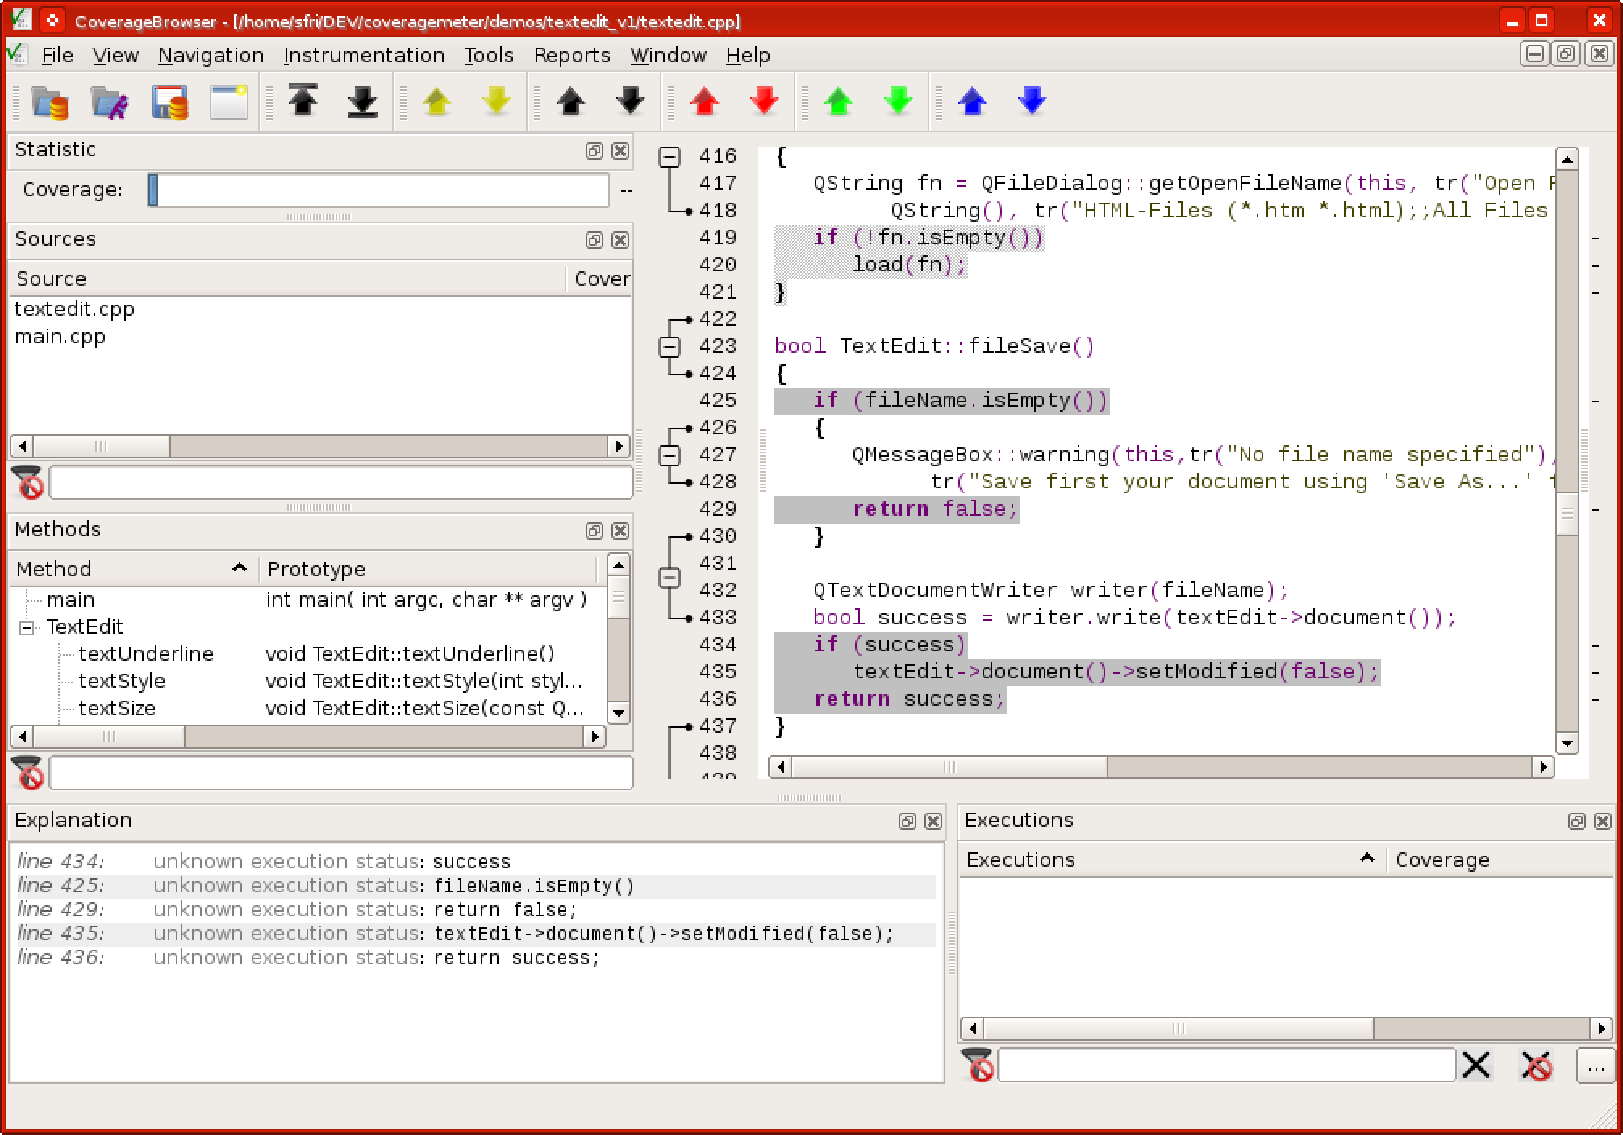
\includegraphics[scale=.5]{coveragebrowser_textedit}
  \end{center}
  \caption{\CoverageBrowser\ after loading \TextEdit\ instrumentation database}
  \label{fig:startup}
\end{figure}

By clicking on \GUIMenuTwo{File}{Load~Execution~Report\ldots}, 
an import dialog appears in which it is necessary to enter at least  the file path of
\verb$textedit.csexe$ (field: 'File~Name') and set  the name of the test (Field: 'Name') to
'\textsf{Start~and~Exit}'.  Also, it is judicious to activate the option
'Delete~after~loading' because the report is no longer necessary after our
import and set 'When~file~becomes~modified' to 'Open~this~dialog' to get this
dialog opened automatically after each test execution.

After the import, the coverage information is now visible:
\begin{itemize}
  \item The coverage statistics for each source, method and for the whole
    application will now have been computed.
  \item The source window is now colored and displays in a green (resp.
    red) background the executed (resp. unexecuted) code part.
  \item The execution list contains now one selected item called
    '\textsf{Start~and~Exit}', our only test execution report.
\end{itemize}

\subsubsection{Interactive testing}

{\CoverageBrowser} indicates that the function \verb$TextEdit::fileSave()$ is not executed.
We will try to validate it interactively, guided by the code coverage analysis.

In the actual output of the source window, all source code lines are marked
with a background in red, which means that they have not been executed. (see
    \autoref{lst:src1})

\begin{listings}[H]
  \scriptsize
\begin{alltt}
bool TextEdit::fileSave()
\{
\colorbox{red}{  if (fileName.isEmpty())}
  \{
    QMessageBox::warning(this,tr("No file name specified"),
      tr("Save first your document using 'Save As...' from the menu"),
      QMessageBox::Ok );
\colorbox{red}{    return false;}
   \}

  QTextDocumentWriter writer(fileName);
  bool success = writer.write(textEdit->document());
\colorbox{red}{  if (success)}
\colorbox{red}{     textEdit->document()->setModified(false);}
\colorbox{red}{  return success;}
\}
\end{alltt}
\caption{{\CoverageBrowser} source view of the function TextEdit::save()}
\label{lst:src1}
\end{listings}

The first test we need to execute:
\begin{enumerate}
  \item start {\TextEdit},
  \item click on the '\textsf{Save}' button: {\TextEdit} displays the error message "Save
    first your document using 'Save As\ldots' from the menu"
  \item and quit.
\end{enumerate}

After importing the coverage report, {\CoverageBrowser} indicates that the '\verb$return false;$'
line just after the call of \verb$QMessageBox::warning()$ has been executed (line
    marked with a green background). But the line '\verb$if (fileName.isEmpty())$' is
marked as partially executed (orange background, see \autoref{lst:src2}).

\begin{listings}[H]
  \scriptsize
\begin{alltt}
bool TextEdit::fileSave()
\{
\colorbox{orange}{  if (fileName.isEmpty())}
  \{
    QMessageBox::warning(this,tr("No file name specified"),
      tr("Save first your document using 'Save As...' from the menu"),
      QMessageBox::Ok );
\colorbox{green}{    return false;}
   \}

  QTextDocumentWriter writer(fileName);
  bool success = writer.write(textEdit->document());
\colorbox{red}{  if (success)}
\colorbox{red}{     textEdit->document()->setModified(false);}
\colorbox{red}{  return success;}
\}
\end{alltt}
\caption{{\CoverageBrowser} source view  after clicking on the 'Save' button of TextEdit.}
\label{lst:src2}
\end{listings}

The explanation window (see \autoref{lst:src3}) gives the information that the
evaluation of the expression '\verb$fileName.isEmpty()$' was true during one execution
but was never false. In order to fulfil this condition it is necessary to click
on  the '\textsf{Save As\ldots}' button,  to set the file name and then
click on the '\textsf{Save}' button.

\begin{listings}[H]
  \scriptsize
  \textcolor{orange}{partially executed}: \texttt{fileName.isEmpty()} \par
\hspace{1cm}
\begin{tabularx}{9cm}{||X||X||} \hline\hline
  \begin{center}\textbf{TRUE}\end{center}          & \begin{center}{\textbf{FALSE}}\end{center}      \\ \hline\hline
  \centerline{\textcolor{green}{yes}} 
  \textit{Execution Count:} 1         \newline
  \textit{Executed by:}               \newline
  \hspace{.4cm}- Save Clicked         &

                                        \centerline{\textcolor{red}{no}} 
                                        \textit{Execution Count:} 0      
                                                                         \\ \hline\hline
\end{tabularx}
\caption{{\CoverageBrowser} explanation window after clicking on the 'Save' button of TextEdit.}
\label{lst:src3}
\end{listings}

After importing the new execution report only one source code line remains
partially untested (see \autoref{lst:src4}). In this case, \CoverageBrowser\ indicates
that the boolean variable '\verb$success$' was never false, this means that writing
the document never fails. Of course it is possible to generate such write failures
and so achieve a 100\% code coverage of this function, but we will choose
another test strategy: implement a unit test and import the execution result
into {\TextEdit} instrumentation database.

\begin{listings}[H]
  \scriptsize
\begin{alltt}
bool TextEdit::fileSave()
\{
\colorbox{green}{  if (fileName.isEmpty())}
  \{
    QMessageBox::warning(this,tr("No file name specified"),
      tr("Save first your document using 'Save As...' from the menu"),
      QMessageBox::Ok );
\colorbox{green}{    return false;}
   \}

  QTextDocumentWriter writer(fileName);
  bool success = writer.write(textEdit->document());
\colorbox{red}{  if (success)}
\colorbox{green}{     textEdit->document()->setModified(false);}
\colorbox{green}{  return success;}
\}
\end{alltt}
\caption{{\CoverageBrowser} source view  after clicking on the 'SaveAs\ldots' and 'Save' button of {\TextEdit}.}
\label{lst:src4}
\end{listings}


\subsubsection{Writing unit tests}

Writing a unit test which sets an illegal filename and execute \verb$fileSave()$ using
\QTestLib\ is pretty easy (see \autoref{lst:src5}).

\begin{listings}[H]
  \scriptsize
\begin{verbatim}
#include "tst_textedit.h"

void TestTextEdit::tst_saveFile() {
  TextEdit textEdit;
  textEdit.fileName="/";
  QVERIFY( ! textEdit.fileSave() );
}

QTEST_MAIN(TestTextEdit);
\end{verbatim}
\caption{{\TextEdit} unit test}
\label{lst:src5}
\end{listings}

To get the instrumentation result of this test into TextEdits own
instrumentation database, the following strategy can be applied:
\begin{enumerate}
  \item Create a {\qmake} project file with code coverage configured identically as for the {\TextEdit}
    project. 
  \item Add a post build rule which automatically executes the test and collects
    the coverage information.
  \item Add a unit test listener which saves into the unit tests own instrumentation database
    the code coverage data and the test status (passed or failed) for each unit test executed.
  \item Import the code coverage report into the {\TextEdit} instrumentation database.
\end{enumerate}

The unit test recompiles itself, and \texttt{textedit.cpp}. To be importable into the \TextEdit\
instrumentation database it is necessary that both  objects (this one from
{\TextEdit} and this one from the unit test) are  identically instrumented.
So we need first to use the same instrumentation option: \verb$--cs-count$,
\verb$--cs-full-instrumentation$ and \verb$--cs-qt4$.

This is unfortunately not enough because per default only source and header
files from the current directory are instrumented. We need to instrument the folder of
{\TextEdit} sources: this is achieved by using the \verb$--cs-include-path$ command line option.

This gives us the {\qmake} project file shown in \autoref{lst:qmake3} which generates
the executable \texttt{tst\_textedit.exe} which then produces the execution report
\texttt{tst\_textedit.csexe}. This can be imported into \texttt{tst\_textedit.exe.csmes}
using \CoverageBrowser.

\begin{listings}[H]
  \scriptsize
\begin{verbatim}
HEADERS         = ../textedit_v1/textedit.h \
                  tst_textedit.h

SOURCES         = ../textedit_v1/textedit.cpp \
                  tst_textedit.cpp

TestCocoon {
 TESTCOCOON_OPTIONS =  --cs-count --cs-full-instrumentation
 TESTCOCOON_OPTIONS += --cs-qt4
 TESTCOCOON_OPTIONS += --cs-output=tst_textedit
 TESTCOCOON_OPTIONS += --cs-include-path=../textedit_v1
 TESTCOCOON_OPTIONS += --cs-exclude-file-regex=qrc_.*

 QMAKE_CXXFLAGS += $$TESTCOCOON_OPTIONS
 QMAKE_CCFLAGS  += $$TESTCOCOON_OPTIONS
 QMAKE_LFLAGS   += $$TESTCOCOON_OPTIONS

 QMAKE_CC=cs$$QMAKE_CC
 QMAKE_LINK=cs$$QMAKE_LINK
 QMAKE_CXX=cs$$QMAKE_CXX
}

\end{verbatim}
\caption{Basic {\qmake} project file for unit test}
\label{lst:qmake3}
\end{listings}

We can automatically execute and import the execution report using a post build
rule. \TestCocoon\ provides on the side a command line tool call \cmcsexeimport\
which import an execution report into an instrumentation database.
The post build rule consists to delete first a previous executed report,
execute the test itself, and finally import it into the execution database of
\verb$tst_textedit$ (see \autoref{lst:qmake4}).


\begin{listings}[H]
  \scriptsize
\begin{verbatim}
TestCocoon {
 unix {
   QMAKE_POST_LINK  = rm tst_textedit_v1.csexe ;
   QMAKE_POST_LINK += ./tst_textedit_v1 ;
   QMAKE_POST_LINK += cmcsexeimport -m tst_textedit_v1.csmes \
                      -e tst_textedit_v1.csexe -t UnitTest
 }
 win32 {
   QMAKE_POST_LINK  = del /F tst_textedit_v1.csexe &
   QMAKE_POST_LINK += tst_textedit_v1.exe &
   QMAKE_POST_LINK += cmcsexeimport -m tst_textedit_v1.exe.csmes \
                      -e tst_textedit_v1.csexe -t UnitTest
 }
}
\end{verbatim}
\caption{Post build rules: importing execution report into unit test's instrumentation database}
\label{lst:qmake4}
\end{listings}

The actual implementation imports coverage data without any information about
the executed tests: an execution called '\textsf{UnitTest}' is created which does
not described which test was executed and if its execution was successful.
To provide this information it is necessary to use the \CoverageScanner\ API to
generate an execution report upon the execution of each test. A sample is
available on the \TestCocoon\
homepage\footnote{\url{http://testcocoon.org/testcoverageobject.cpp} and
\url{http://testcocoon.org/testcoverageobject.h}}. Using it is easy: 
\begin{itemize}
  \item Add the two source files in \qmake\ project file (see \autoref{lst:qmake5}).
  \item Instead of inheriting the unit test from \texttt{QObject}, inherit it
    from \texttt{TestCoverageObject} (see \autoref{lst:hdr1}).
\end{itemize}

\begin{listings}[H]
  \scriptsize
\begin{verbatim}
HEADERS += testcoverageobject.h
SOURCES += testcoverageobject.cpp
\end{verbatim}
\caption{Including \CoverageScanner\ listener into {\qmake} project file}
\label{lst:qmake5}
\end{listings}

\begin{listings}[H]
  \scriptsize
\begin{verbatim}
#include "testcoverageobject.h"
#include "../textedit_v1/textedit.h"
#include <QtTest/QtTest>

class TestTextEdit : public TestCoverageObject
{
    Q_OBJECT
  private slots:
    void tst_saveFile();
};
\end{verbatim}
\caption{\TextEdit\ unit test header}
\label{lst:hdr1}
\end{listings}

A small look in \texttt{testcoverageobject.cpp} (see \autoref{lst:src6}) lets
us understand how it works: it only provides a \verb$cleanup()$ function to
\QTestLib, which is executed after each unit test item.
The code between \verb$#ifdef __COVERAGESCANNER__$ and \verb$#endif$ is 
compiled when \CoverageScanner\ is invoked\footnote{\texttt{\_\_COVERAGESCANNER\_\_} define
is set automatically when using \CoverageScanner\ and so does not need to be
defined}. It builds a test name using the object name and the test function
name. In our case, an execution item \verb$unittest/TestTextEdit/tst_saveFile$
is generated. The slash permits to organize the tests in a tree view.
The current test status (``PASSED'' or ``FAILED'') is recorded, and
committed to the execution report by calling \verb$__coveragescanner_save()$.


\begin{listings}[H]
  \scriptsize
\begin{verbatim}
.....
void TestCoverageObject::cleanup()
{
  cleanupTest();
#ifdef __COVERAGESCANNER__
  QString test_name="unittest/";
  test_name+=metaObject()->className();
  test_name+="/";
  test_name+=QTest::currentTestFunction();
  __coveragescanner_testname(test_name.toLatin1());
  if (QTest::currentTestFailed())
    __coveragescanner_teststate("FAILED"); 
  else 
    __coveragescanner_teststate("PASSED") ; 
  __coveragescanner_save();
  __coveragescanner_testname(""); 
#endif
}
\end{verbatim}
\caption{\texttt{TestCoverageObject} source code}
\label{lst:src6}
\end{listings}

At this stage we could start \CoverageBrowser, load the \TextEdit\ instrumentation
database and import the instrumentation database of the unit test
\GUIMenuTwo{File}{Import Unit Tests\ldots}, but we can also use \cmmerge\ to
automate this step. \cmmerge\ permits us  to import the execution report from one
instrumentation database into another. So it is possible to call it in
the post build rules to import the coverage information into \TextEdit\
database automatically (see \autoref{lst:qmake6}).

\begin{listings}[H]
  \scriptsize
\begin{verbatim}
TestCocoon {
 # Merge coverage database into TextEdit database
 unix {
   QMAKE_POST_LINK += ;
   QMAKE_POST_LINK += cmmerge -o ../textedit_v1/textedit.tmp \
                   -i ../textedit_v1/textedit.csmes ./tst_textedit_v1.csmes &&
   QMAKE_POST_LINK += rm ../textedit_v1/textedit.csmes &&
   QMAKE_POST_LINK += mv ../textedit_v1/textedit.tmp ../textedit_v1/textedit.csmes 
 }
 win32 {
   QMAKE_POST_LINK += &
   QMAKE_POST_LINK += cmmerge -o ../textedit_v1/textedit.tmp \
                   -i ../textedit_v1/textedit.csmes ./tst_textedit_v1.csmes &&
   QMAKE_POST_LINK += DEL /F ../textedit_v1/textedit.csmes &&
   QMAKE_POST_LINK += REN ../textedit_v1/textedit.tmp ../textedit_v1/textedit.csmes 
 }
}
\end{verbatim}
\caption{Post build rules: merging instrumentation results into \TextEdit\ instrumentation database}
\label{lst:qmake6}
\end{listings}

After building the unit test, the function \verb$fileSave()$ is displayed as
100\% covered by CoverageBrowser and the execution list contains our 3 manual
tests and one unit test. (see \autoref{fig:execlist1})

\begin{figure}[H]
  \begin{center}
    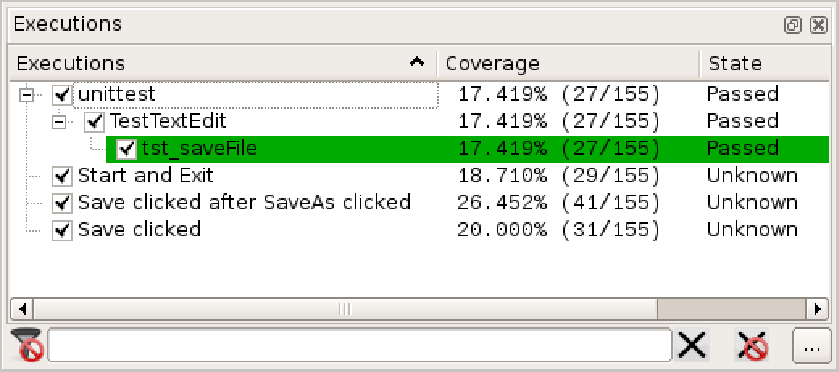
\includegraphics[scale=.5]{textedit_list_of_tests}
  \end{center}
  \caption{Execution list after execution of all tests}
  \label{fig:execlist1}
\end{figure}


\subsection{Working with code coverage data}

In most of the cases, the code coverage technology is only used by the
developer to find untested code portions and by the management to produce test
status diagrams. 

\TestCocoon\ provides some features which permit you to extend the application
area of the code coverage technique.


\subsubsection{Post mortem analysis}

Recording the coverage data of each test permits to compare it together and
answer the question: ``what does this test cover more than another?''. This is
particularly useful if one test fails and the developer wants to identify which
code part is involved.

For example, lets have a look at the \TextEdit\ sample. Clicking on '\textsf{Save}' generates
an error message telling us that no file name was defined. This is ergonomically
interesting since that
\TextEdit\ could also open directly the '\textsf{SaveAs\ldots}' dialog. 

To identify which code part is impacted, we simply compare the '\textsf{Save Clicked}'
execution to all other which involve the '\textsf{Save}' button. First it is necessary
to switch into the ``Execution Benefit Analysis'' mode
(Menu: \GUIMenuTwo{Tools}{Execution Benefit Analysis}). In the execution list select
the tests ``\textsf{tst\_saveFile}'' and ``\textsf{SaveAs clicked before Save clicked}''. Double
click on ``\textsf{Save clicked}'' execution: the execution comparison symbol appears in
front of its name (see \autoref{fig:execlist2}).

\begin{figure}[H]
  \begin{center}
    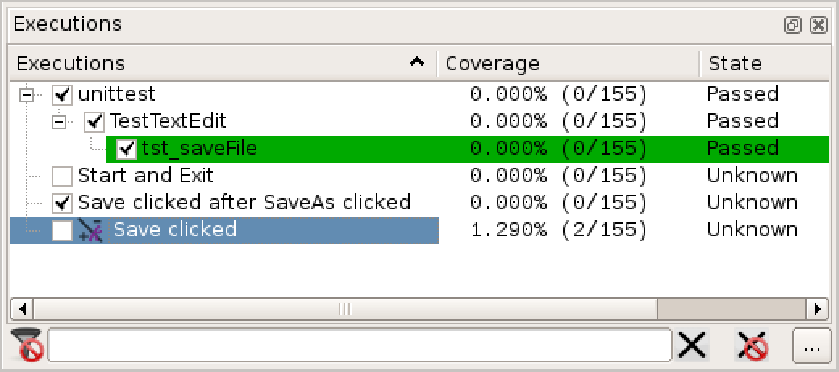
\includegraphics[scale=.5]{textedit_list_of_tests_benefit}
  \end{center}
  \caption{Execution list when comparing executions together}
  \label{fig:execlist2}
\end{figure}

In this mode the coverage analysis is made only on source code lines which are
not executed by ``\textsf{tst\_saveFile}'' and ``\textsf{SaveAs clicked before Save clicked}''.
That's why the overall coverage decreases to 1.3\% which means in this case
that ``\textsf{Save clicked}'' executes 1.3\% more code than the selected tests. 

A deeper look on the source code shows that  only two lines of the
\verb$TextEdit::fileSave()$ function (see \autoref{lst:src10}) are not grayed:
the lines which pop-up the error message. This are the lines that needs to be
modified to change the behaviour behind the ``\textsf{Save}'' button.

\begin{listings}[H]
  \scriptsize
\begin{alltt}
bool TextEdit::fileSave()
\{
\colorbox{orange}{  if (fileName.isEmpty())}
  \{
    QMessageBox::warning(this,tr("No file name specified"),
      tr("Save first your document using 'Save As...' from the menu"),
      QMessageBox::Ok );
\colorbox{green}{    return false;}
   \}

  QTextDocumentWriter writer(fileName);
  bool success = writer.write(textEdit->document());
\colorbox{Graylight}{  if (success)}
\colorbox{Graylight}{     textEdit->document()->setModified(false);}
\colorbox{Graylight}{  return success;}
\}
\end{alltt}
\caption{{\CoverageBrowser} source view of the benefit of the execution ``Save clicked''.}
\label{lst:src10}
\end{listings}

Correcting the \verb$fileSave()$ function is trivial and consists only to
replace the call of \verb$QMessageBox::warning()$ through \verb$fileSaveAs()$.
(see \autoref{lst:src11})

\begin{listings}[H]
  \scriptsize
\begin{verbatim}
bool TextEdit::fileSave()
{
   if (fileName.isEmpty())
     return fileSaveAs();

   QTextDocumentWriter writer(fileName);
   bool success = writer.write(textEdit->document());
   if (success)
      textEdit->document()->setModified(false);
   return success;
}
\end{verbatim}
\caption{\TextEdit\ with a modified \texttt{fileSave()} function.}
\label{lst:src11}
\end{listings}

\subsubsection{\label{sec:patchimpact}Evaluation of the impact of a hot fix}

Before committing a change or starting to test a hot fix, it is possible to
estimate the impact of the code modification. \CoverageBrowser\ is able
to perform an analysis on the difference between two source sets and so lists
which tests are or are not impacted.

Start \CoverageBrowser\ and load the instrumentation database of the  original
\TextEdit\ sample. Then click on \GUIMenuTwo{Tools}{Compare with\ldots} and
select the modified version of \TextEdit\ instrumentation database.
\CoverageBrowser\ displays  now the source code like a text comparison
application.

Clicking on \GUIMenuTwo{Tools}{Analysis on Modified Methods} permits to exclude
all unmodified functions from the coverage analysis. In our case, it is as if
only the function \verb$TextEdit::fileSave()$ was instrumented. (see \autoref{fig:patchimpact})
This also impacts the statistic calculations: the coverage statistic of an
execution is also limited only to this function. Some executions have now a
coverage statistic which is not zero, these tests are impacted by the code
modification we made. 

In our case:
\begin{itemize}
  \item ``Save clicked'',
  \item ``SaveAs clicked before Save clicked'' and 
  \item ``tst\_saveFile'' (our unit test).
\end{itemize}

``Start and Exit'' has a coverage equal to 0\% and so does not execute our
patched code.

In other words, only two manual tests and one unit test need to be re-executed
to ensure that no regressions are generated.

\begin{figure}[H]
  \begin{center}
    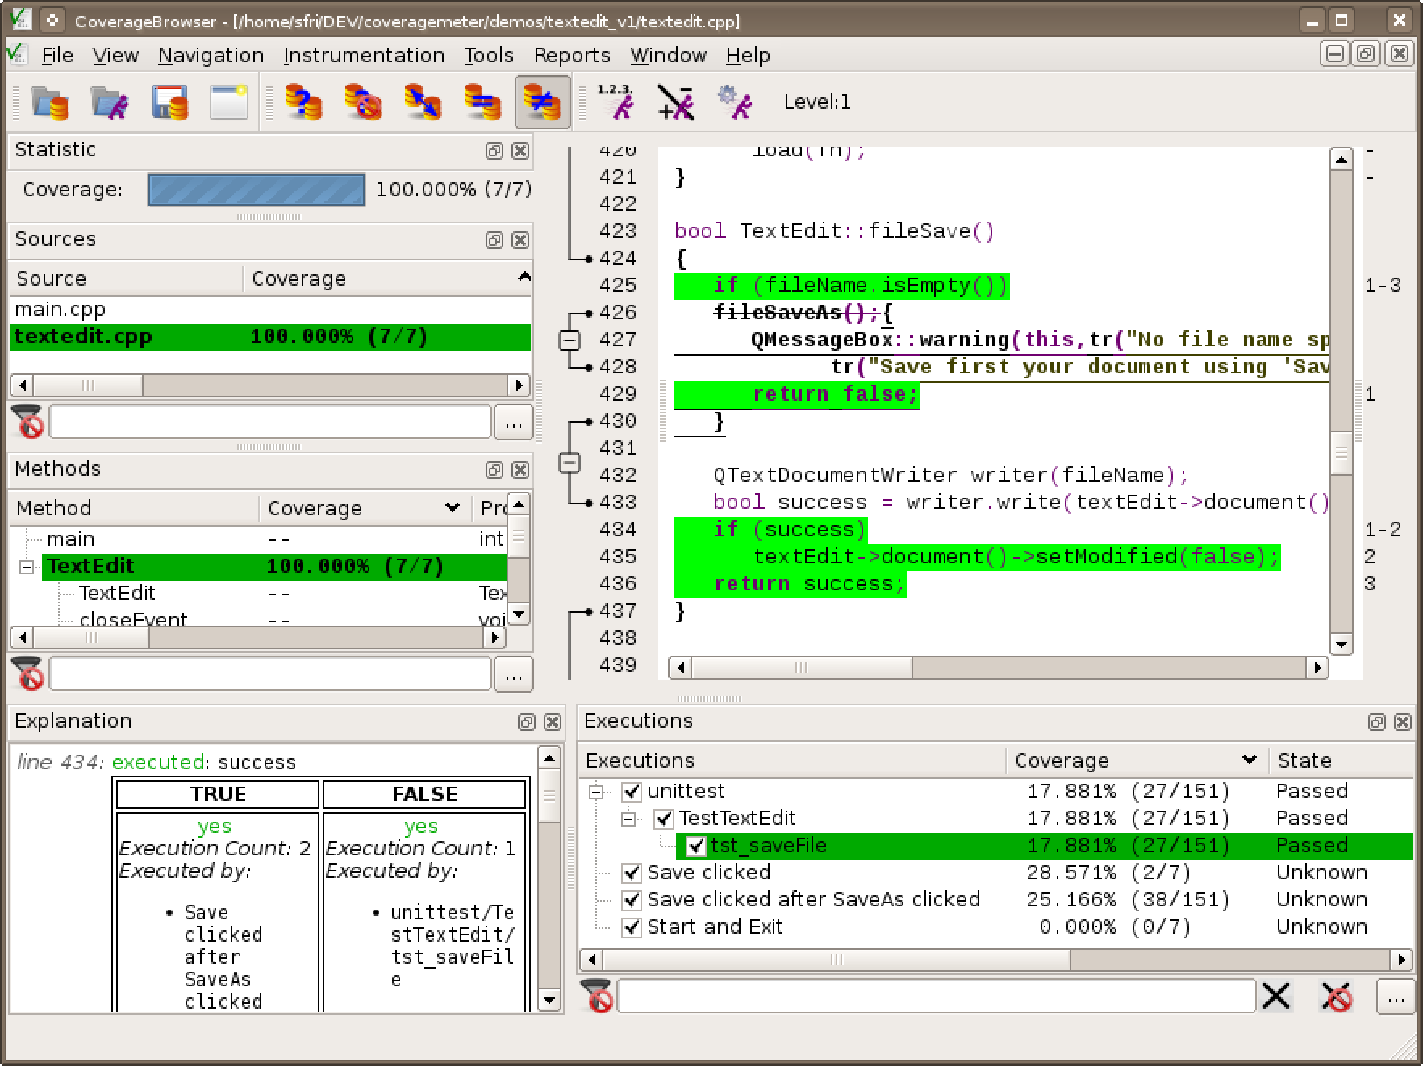
\includegraphics[scale=.5]{textedit_patch_impact}
  \end{center}
  \caption{List of tests impacted by a modification}
  \label{fig:patchimpact}
\end{figure}

\subsubsection{Black-box testing/distributed testing}

To test the new version of \TextEdit\ we decide to perform what is called  black-box testing.
This kind of testing consists of testing without having access to or knowledge of the code. But, contrary to what you would believe,
the code coverage analysis is still possible. 

\TestCocoon\ gives the possibility to generate a
black-box database which does not contain the source code. 
Simply click on \GUIMenuTwo{File}{Generate Black-Box Configuration\ldots} to
generate a new instrumentation database. This database, with \TextEdit\
executable, can be transmitted to the test team which can then use it with a
simplified version of \CoverageBrowser\ (see \autoref{fig:blackbox}): only
importing and the managing execution report are possible.

\begin{figure}[h]
  \begin{center}
    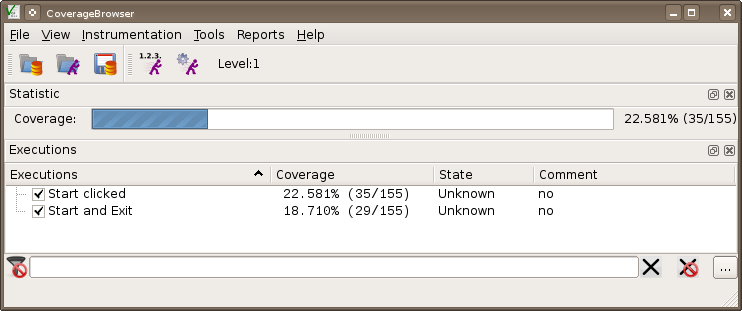
\includegraphics[scale=.5]{textedit_blackbox}
  \end{center}
  \caption{Black-box testing using \CoverageBrowser}
  \label{fig:blackbox}
\end{figure}


Once all tests are  finished, this black-box database can be merged into the original
\TextEdit\ database using \CoverageBrowser\ merge facilities (Menu:
\GUIMenuTwo{File}{Merge width\ldots}).

\subsubsection{Verifying if a bug fix is correctly tested}

Generally, when a small bug fix is made, the most important part of the source
code remains unchanged, and so retesting the whole application is generally not
necessary. \TestCocoon\ is able to work on only the modified source code
between two software versions\footnote{see \nameref{sec:patchimpact}, page
\pageref{sec:patchimpact}} and so focus the analysis on the patch. Simply
load the instrumentation database of the newest \TextEdit\ version, compare it
to the first version and activate the analysis on modified functions.

\begin{figure}[h]
  \begin{center}
    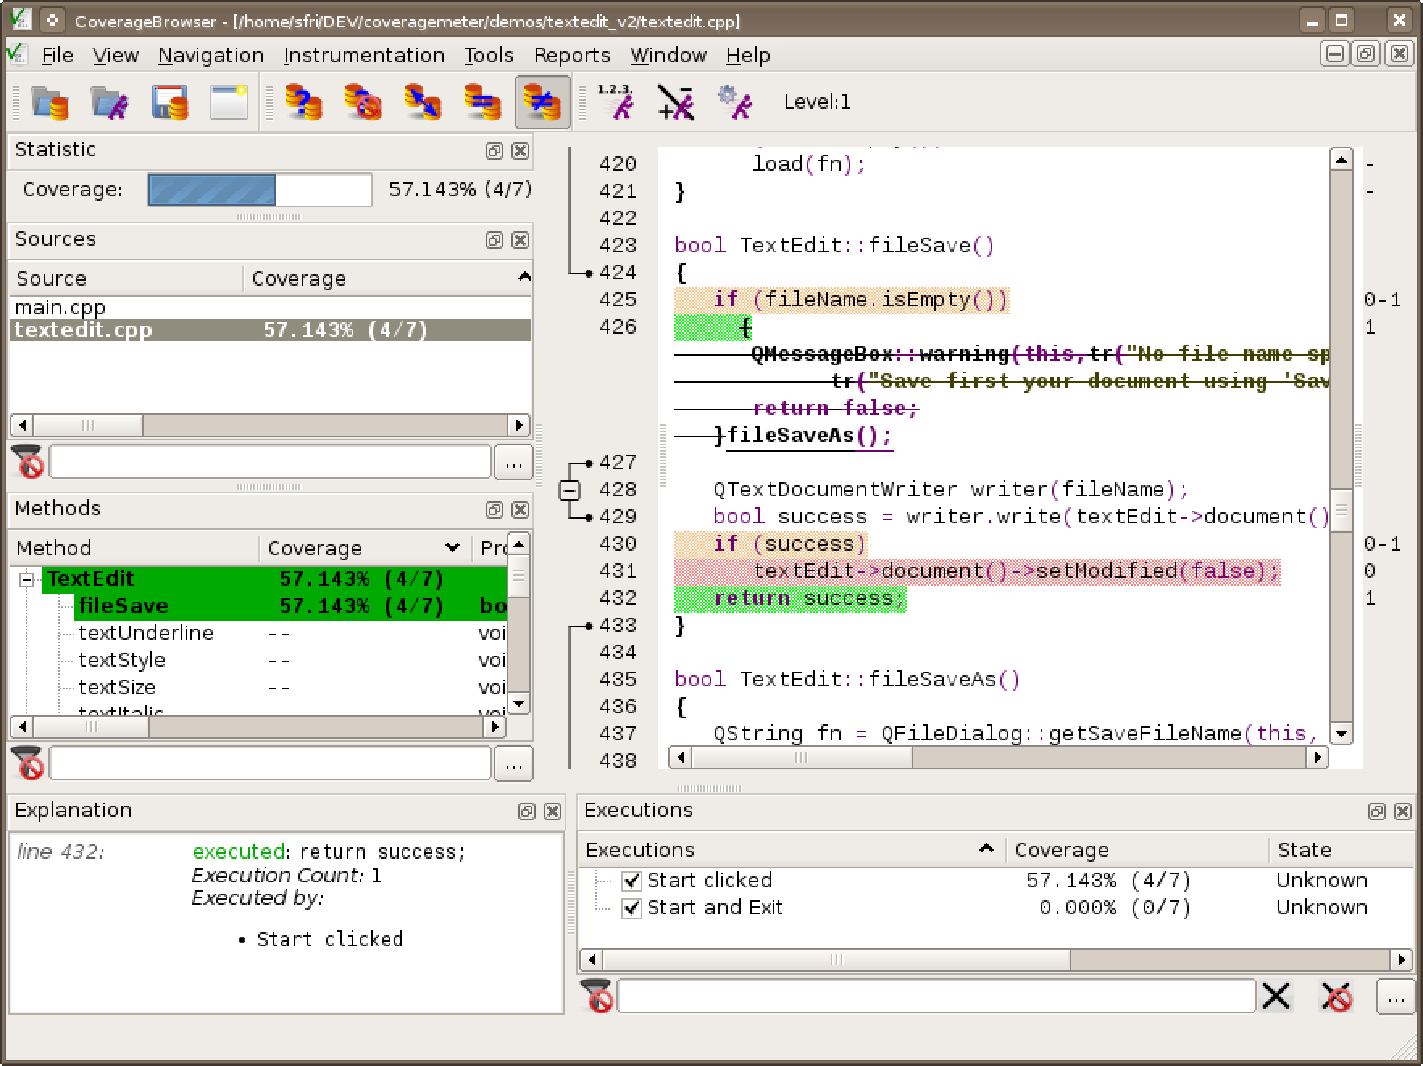
\includegraphics[scale=.5]{textedit_patch_coverage}
  \end{center}
  \caption{Coverage of the patched function}
  \label{fig:patchcoverage}
\end{figure}

The result is visible in \autoref{fig:patchcoverage}: the two tests ``Start
clicked'' and ``Start and Exit'' are covering 57\% of
\verb$TextEdit::fileSave()$ function, the only modified method from our fix.

\section{Conclusion}

  \TestCocoon\ provides code coverage analysis which can be applied to
the majority of testing techniques: unit, manual and
black-box testing. Its analysis ignores the code generated by Qt tools 
(\moc, \qrc\ and \uic) and so instruments only the code generated by and of interest to
developers. The test results can be collected into one database
and can be used to evaluate the test progress of a complete application.
Also it helps to estimate the impact of a code
modification and measure the testing level of patch without retesting
the whole application again.


\part{\CoverageBrowser\ Reference Manual} \cutname{coveragebrowser.html}

\chapter{Introduction} 

\CoverageBrowser\ is the graphical interface which enables the user to analyze 
test coverage. \par\bigskip
The typical usage of coverage browser consists in:
\begin{enumerate}
  \item Loading the instrumentation database ("\verb$.csmes$" file) 
        which is generated by \CoverageScanner.
  \item Loading the execution report ("\verb$.csmes$"' file).
        \CoverageBrowser\ displays them in a tree view and enables the user to individually select
        or deselect them for coverage analysis.
  \item Searching for untested code segments and executing a test.
  \item Marking dead code or code which can not be tested, as "manually validated".
  \item Commenting instrumented code areas.
\end{enumerate}

\CoverageBrowser\ saves all data (execution reports, comments, \ldots)
to the instrumentation database.  


\chapter{\label{coveragebrowser-black-box}Black box and white box testing}

\CoverageBrowser\ can be used for white box and black box testing: if no source
code information is available in the instrumentation database (\verb$.csmes$ file),
\CoverageBrowser\ switch in a lightweight version. In this mode, it is not possible to have access to 
the source code or to the symbol information, but the user can import and manage its executions.
\bigskip\\
A black box instrumentation database can generated by clinging on \GUIMenuTwo{File}{Generate Black Box Configuration}.
This instrumentation can be in a second step merged in a white box configuration again.


   \InsertPictureDescription{coveragebrowser_blackbox}{\CoverageBrowser\ view when performing black box tests}

\chapter{\label{executions-list}Execution Management Window} \label{execution-management}

\section{Principle}

 Executions of the instrumented application are managed in a tree view in the \GUIwindow{Executions} window.
 \CoverageBrowser\ uses a slash {\tt '/'} as separator for grouping measurements together.\\
 For example, tests viewed in figure \seeref{fig:coveragebrowser_executions_fig}
 have the following names:\\
 \begin{itemize}
 \item {\tt SubTest/test1}
 \item {\tt SubTest/test2 (12)}
 \item {\tt SubTest/test2 (2)}
 \end{itemize}


   \InsertPictureDescription{coveragebrowser_executions_fig}{Executions View}

 
 The check-box next to each item can be used to select executions. 
 The input field \GUIicon{filter} permits to filter the output using regular expressions \seechapref{sec:coveragebrowser-filter} and the button button \GUIicon{select} and  \GUIicon{deselect} permits to select/unselect
 all executions visible. Additional filter which concerns the execution state and the comments can be set using the button \GUITextButton{...}.
 The item text which can be filtered is the full name of the execution. (example:~\verb$SubTest/test1$)\\
   
 The \GUIwindow{Source Browser}, \GUIwindow{Method Browser} and the \GUIwindow{Source Viewer} windows display only the code coverage status
 of the selected executions. The button \GUIicon{testPerformance} permits to switch into the test benefit analysis mode \seechapref{test-benefit}.\\

 The user can set the state of the executed test, which can be:
   \begin{description}
    \item[\GUIitem{Unknown}] 
         Default state. 
    \item[\GUIitem{\textcolor{green}{Passed}}]  
         This state is used to mark the test as passed (background colour is \textcolor{green}{green})
    \item[\GUIitem{\textcolor{red}{Failed}}]  
         This state is used to mark the test as failed (background colour is \textcolor{red}{red}) 
    \item[\GUIitem{\textcolor{orange}{Need manual check}}] 
         This state is used to show the test has to be checked manually (background colour is \textcolor{orange}{orange}) 
   \end{description}

 Using the context menu or the appropriate docking window, it is possible to comment, rename, delete or merge\footnote{After merging the executions used as source are deleted} executions together.
 \CoverageBrowser\ provides the possibility to use regular expressions for this manipulations. The syntax of it is described in the chapter \seeref{sec:coveragebrowser-filter} and a preview of the operation is calculated automatically. \\
Here some examples of deleting execution:
\begin{itemize}
 \item To delete all execution using the wildcard syntax: \newline
      \begin{tabular}{ll}
       Execution Name   & \verb$*$           \\
      \end{tabular} 
 \item To delete all executions in \verb$TESTS$ using the wildcard syntax: \newline
      \begin{tabular}{ll}
       Execution Name   & \verb$TESTS/*$           \\
      \end{tabular} 
 \item To delete all executions in \verb$TESTS$ using the regular expression syntax: \newline
      \begin{tabular}{ll}
       Execution Name   & \verb$=TESTS/.*$           \\
      \end{tabular} 
\end{itemize}
Here some examples of renaming execution:
\begin{itemize}
 \item To put all executions in the directory \verb$TESTS$ set: \newline
      \begin{tabular}{ll}
       Actual Execution Name   & \verb$=.*$           \\
       New Execution Name      & \verb$TESTS/&$       \\
      \end{tabular} 
 \item To move all executions in the directory \verb$TESTS$ in the directory \verb$OLD$ set: \newline
      \begin{tabular}{ll}
       Actual Execution Name   & \verb$=TESTS/(.*)$           \\
       New Execution Name      & \verb$OLD/\1$       \\
      \end{tabular} 
 \item To rename all executions in all directories in \verb$testname [directory]$ set: \newline
      \begin{tabular}{ll}
       Actual Execution Name   & \verb$=([^/]*)/([^/]*)$           \\
       New Execution Name      & \verb$\2 [\1]$       \\
      \end{tabular} 
\end{itemize}

   \InsertPictureDescription{coveragebrowser_rename_regex_fig}{Renaming using Regular Expressions}

\NOTE{The name of the test item and also its state can be defined by an external test suite.\seechapref{test-suite-adaptation}}

\section{\label{load-execution-report}Loading an Execution Report}
   The execution report is produced upon application exit. 
   Its name is defined by the initialization function 
   \verb$__coveragescanner_install$ of the \CoverageScanner\ library 
   \seechapref{coveragescanner_install}\index{\_\_coveragescanner\_install}. 
   Its extension is followed by "{\tt .csexe}".
   It contains the list of all executed code segments for each application run.
   The execution report is never overwritten but 
   execution contents are appended. \index{Execution Report}\bigskip

   To load an execution report click on \GUIMenuTwo{File}{Load Execution Report} 
   or the icon \GUIicon{csexeopen} on the toolbar. 
   The dialog as shown in \seeref{fig:coveragebrowser_loadexec_fig} will appear.\\
   \index{Load Execution Report}
   \InsertPictureDescription{coveragebrowser_loadexec_fig}{Loading Execution Report Dialog}
   The file can be loaded directly or using a script.
   To load directly, click on \GUIitem{file}, 
   enter the path of the "{\tt .csexe}" file to load 
   to the free form input box or use the browse button. \\
   If the option \GUIitem{Delete after transferring} is selected, the execution report file 
   will be deleted after transfer. 
   The option \GUIitem{When file becomes modified} permits to reopen this dialog 
   automatically when the execution report is modified.
   \bigskip

   The \GUIitem{Name} field allows the user to specify the name of the imported instrumentation
   if this is not specified in the execution report \seechapref{executionreportname}. Also, it is
   possible to set the execution status (passed, failed or to be checked manually) of all imported executions. \\
   If more than one instrumentation is imported an index is appended to this default name. \\
   
   The option \GUIitem{Import Preprocessing} permits to select the behaviour
   in the case of conflicts or redundant executions:
   \begin{description}
   \item[\GUIitem{Ignore Duplicate Executions}]
     Executions which have executed the same code than an execution which are already 
     imported are ignored.
   \item[\GUIitem{Import Duplicate Executions}]
     Executions are imported if at least one instrumented source code line is executed.
   \item[\GUIitem{Import Duplicate And Empty Executions}]
     All executions are imported.
   \item[\GUIitem{Merge all executions with the same name together}]
     All executions with the same name are merged (i.e. the execution count of each instrumentation is added).
   \end{description}


   Invalid executions are not imported and 
   a summary shows when the operation is completed (see figure \seeref{fig:coveragebrowser_loadreport})
   when \GUIitem{Display import summary} option is selected. \bigskip
   \InsertPictureDescription{coveragebrowser_loadreport}{Loading Executions - Summary}

   If the execution report is not accessible through the file system,
   a script can be used. The script has only to print the contain of 
   the execution report to the standard output (\verb$stdout$). The standard error
   output (\verb$stderr$) is displayed on the screen and can be used for debugging
   purpose. On success, the script must exit with the value \verb$0$.

\section{\label{test-benefit}Test Benefit Analysis Mode}
 The test benefit analysis mode if activated by clicking on the button \GUIicon{testPerformance}.
 In this mode, \CoverageBrowser\ does not display the coverage of a set of tests but the lines 
 covered by an execution which are not covered by a set of reference executions.
 In other words, \CoverageBrowser\ shows what an execution is covering more than a set of other executions. \\

 The list of reference executions are the executions checked in the execution list. 
 Double-clicking on the name of the execution permits to select the test to analyse.
 Only the instrumented lines which are executed by this execution are shown, the other are in the state "hidden".
 Also the coverage statistics displayed in the source list are only containing the percentage of 
 instrumented statements which are only executed by this the selected execution.

 \NOTE{If the execution to analyse is present in the list of reference executions, 
       this one if implicitly remove from the list. (In other words, if execution A 
           is compared to execution A and B,
           \CoverageBrowser\ make a comparison of execution A with B only.)
      Comparing the benefit of an execution with itself will in fact not give usefully information.}

 \InsertPictureDescription{coveragebrowserbenefit_fig}{Test Benefit Analysis Mode}

\chapter{Source Browser Window} \label{source-browser}

 \NotForBlackBoxTesting
 The \GUIwindow{Source Browser} window can be displayed by clicking 
   on \GUIMenuTwo{View}{Source Browser}. \\
   \InsertPictureDescription{coveragebrowser_srclst_fig}{Source Browser Window}
   Each item is a \CorCPlusPlus\ source file and the sub-entries are the list 
   of included headers which have been instrumented. When an item 
   the \GUIwindow{Source Window} will be displayed.
 \newline

  The \GUIwindow{Source Browser} window displays rudimentary code coverage statistics
  for each source code file. The color of each item is selected according to code coverage
  statistics for each file and the watermarks.\seechapref{watermarks} \\

 The input field \GUIicon{filter} permits to filter the output using regular expressions 
   \seechapref{sec:coveragebrowser-filter}.
 The item text which can be filtered is the full path of the source file. (example:~\verb$c:\directory\file.cpp$)\\

\begin{tableenv}
    \begin{center}
    \begin{tabularx}{\linewidth}{|c|c|X|}
    \hline
        \textbf{Icon}            & \textbf{Shortcut}       & \textbf{Description} \\ \hline
        \GUIicon{previousModule} & \Shortcut{Ctrl+Shift+F} & Previous source file \\ \hline
        \GUIicon{nextModule}     & \Shortcut{Ctrl+F}       & Next source file     \\ \hline
    \end{tabularx}
    \caption{Source Browser - Shortcuts}
    \label{source_list_shortcut}
    \end{center}
\end{tableenv}


 \NotForBlackBoxTesting
\chapter{Method Browser Window} \label{method-browser}

 The \GUIwindow{Method Browser} window can be opened by clicking 
   on \GUIMenuTwo{View}{Method Browser}. \\

   \InsertPictureDescription{coveragebrowser_method_list}{Method Browser Window}
 The \GUIwindow{Method Browser} window displays a the code coverage
 statistics of each \CorCPlusPlus\ functions, classes and namespaces.
 Clicking on a function permits to show all instrumented lines of it
 in the \GUIwindow{Source Viewer}.\\

 The input field \GUIicon{filter} permits to filter the output using regular expressions 
   \seechapref{sec:coveragebrowser-filter}.
 The item text which can be filtered is the symbol name including the class name and the namespace.
 (example:~\verb$MyNamespace::MyClass::MyProc$)

 \NotForBlackBoxTesting
\chapter{Source Viewer Window} \label{source-viewer}

\section{Source Display}

 The \GUIwindow{Source Viewer} window can be displayed by clicking on \GUIMenuTwo{View}{New Source Window}.

\InsertPictureDescription{coveragebrowser_source_desc}{Source Window}

 The \GUIwindow{Source Viewer} window displays the source file or its \CorCPlusPlus\ preprocessed view. 
 Clicking on \GUIicon{preprocessorview} enables the user to toggle between the 2 different views. \bigskip \\

 The source code is colored with code coverage instrumentations. 
 The colors used are described in section \seeref{sec:color_convension}.  \bigskip \\

 By selecting an area with the mouse, corresponding instrumentations are highlighted and a 
 detailed description of them is displayed in the \GUIwindow{Explanation} 
 window \seechapref{code-coverage-explanation}.  It is possible to navigate between 
 instrumentations using the navigation buttons \GUIicon{nextInstrumentation} 
 and \GUIicon{previousInstrumentation}. 
 Navigation buttons in yellow, blue, red and green permit to jump to the next or previous
 comments, manually validated instrumentations, non-executed code parts or executed code parts.
  Clicking on the source code selects the nearest instrumentation. \bigskip \\
 

 If a comment is entered for an instrumentation, the icon \GUIicon{comments} is displayed in the margin.  \\

 On the right side, \CoverageBrowser\ displays the \index{Test coverage count} test coverage 
 count\footnote{The test coverage count is obtained by generating 
 the instrumentation with \CoverageScanner\ using the option 
 \CMDoption{hit}}
 or the \index{Code coverage count} code coverage count\footnote{The 
 code coverage count is obtained by generating 
 the instrumentation with \CoverageScanner\ using the option 
 \CMDoption{count}}
 for each line.
 If a source code line contains more than one instrumentation,
 \CoverageBrowser\ display the range of their counts.

\begin{tableenv}
    \begin{center}
    \begin{tabularx}{\linewidth}{|l|X|}
    \hline
        \textbf{Mouse Wheel} & \textbf{Description} \\ \hline
        \Shortcut{Wheel} & Scroll up/down \\ \hline
        \Shortcut{Ctrl+Wheel} & Zoom in/out\\ \hline
        \Shortcut{Shift+Wheel} & Next/previous instrumentation \\ \hline
    \end{tabularx}
    \caption{Source Display - Mouse Wheel}
    \label{source_display_mousewheel}
    \end{center}
\end{tableenv}

\begin{tableenv}
    \begin{center}
    \begin{tabularx}{\linewidth}{|c|c|X|}
    \hline
        \textbf{Icon}                                      & \textbf{Shortcut}     & \textbf{Description}                                         \\ \hline
        \GUIicon{previousInstrumentationComment}           & \Shortcut{Ctrl+Shift+B} & Previous comment                                             \\ \hline
        \GUIicon{nextInstrumentationComment}               & \Shortcut{Ctrl+B}       & Next comment                                                 \\ \hline
        \GUIicon{previousInstrumentationUnTested}          & \Shortcut{Ctrl+Shift+U} & Previous unexecuted code                                     \\ \hline
        \GUIicon{nextInstrumentationUnTested}              & \Shortcut{Ctrl+U}       & Next unexecuted code                                         \\ \hline
        \GUIicon{previousInstrumentationTested}            & \Shortcut{Ctrl+Shift+T} & Previous executed code                                       \\ \hline
        \GUIicon{nextInstrumentationTested}                & \Shortcut{Ctrl+T}       & Next executed code                                           \\ \hline
        \GUIicon{previousInstrumentationManuallyValidated} & \Shortcut{Ctrl+Shift+V} & Previous manually validated instrumentation                  \\ \hline
        \GUIicon{nextInstrumentationManuallyValidated}     & \Shortcut{Ctrl+V}       & Next manually validated instrumentation                      \\ \hline
        \GUIicon{previousInstrumentation}                  & \Shortcut{Ctrl+Shift+I} & Previous instrumentation                                     \\ \hline
        \GUIicon{nextInstrumentation}                      & \Shortcut{Ctrl+I}       & Next instrumentation                                         \\ \hline
        \GUIicon{previousModule}                           & \Shortcut{Ctrl+Shift+F} & Previous source file                                         \\ \hline
        \GUIicon{nextModule}                               & \Shortcut{Ctrl+F}       & Next source file                                             \\ \hline
        \GUIicon{newview}                                  & \Shortcut{Ctrl+J}       & Open a new source window                                     \\ \hline
        \GUIicon{preprocessorview}                         & \Shortcut{Ctrl+Shift+J} & Switch between the preprocessor view and the original source \\ \hline
        \GUIicon{comments}                                 & \Shortcut{Ctrl+K}       & Add/Edit Comments                                            \\ \hline
        \GUIicon{no_comments}                              & \Shortcut{Ctrl+Shift+K} & Remove Comments                                              \\ \hline
        \GUIicon{validation}                               & \Shortcut{Ctrl+W}       & Mark as Validated                                            \\ \hline
        \GUIicon{no_validation}                            & \Shortcut{Ctrl+Shift+W} & Clear Validation Flag                                        \\ \hline
        \GUIicon{commentundo}                              & \Shortcut{Ctrl+Z}       & Undo                                                         \\ \hline
        \GUIicon{commentredo}                              & \Shortcut{Ctrl+Shift+Z} & Redo                                                         \\ \hline
    \end{tabularx}
    \caption{Source Display - Shortcuts}
    \label{source_display_shortcut}
    \end{center}
\end{tableenv}

 \NotForBlackBoxTesting
\section{Color Convention} \label{sec:color_convension}
Instrumentations are displayed in a source window using different colors:
\begin{description}
  \item[\textcolor{green}{Green - \GUIitem{Executed}}] \index{Color!Red} \index{Status!Executed}
                                An instrumentation is displayed in green when the code has been executed.
  \item[\textcolor{orange}{Orange - \GUIitem{Partially Executed}}] \index{Color!Orange} \index{Status!Partially Executed}
                                An instrumentation is marked as "{\tt Partially Executed}" when it 
                                is not completely executed. This occurs when
                                a Boolean expression was only true or false for example.
                                In the case of a source code line which contains more than one instrumentation, 
                                the line is marked as "{\tt Partially Executed}" when one of its instrumentations
                                has not been "{\tt Executed}".
                                A detailed information is displayed in the 
                                \GUIwindow{Explanation} window \seechapref{code-coverage-explanation}.
  \item[\textcolor{red}{Red - \GUIitem{Never Executed} or \GUIitem{Execution count too low}}] \index{Color!Red} \index{Status!Never Executed} \index{Status!Execution count too low}
                                An instrumentation is displayed in red when the code is never executed
                                or when the execution count is lower that than the execution count requested.

  \item[\textcolor{blue}{Blue - \GUIitem{Manually Set To Be Executed}}] \index{Color!Blue} \index{Status!Manually Set To Be Executed}
                                The user has the possibility to mark an instrumentation as '{\tt Manually Validated}'.
                                This is usually to exclude dead code or code which 
                                cannot be tested for code coverage statistics.
                                This state is only relevant if executions are in a
                                "{\tt Never Executed}" or "{\tt Partially Executed}" state.
  \item[\textcolor{Gray}{Gray - \GUIitem{Unknown} or \GUIitem{Hidden}}] \index{Color!Gray} \index{Status!Hidden}\index{Status!Unknown}
                                Gray is used when no information about instrumentation is available.
                                This occurs when no executions are selected or when analysing the benefit
                                of tests \seechapref{test-benefit}.
  \item[\textcolor{magenta}{Magenta - \GUIitem{Registration Needed}}] \index{Color!Magenta} \index{Status!Registration Needed}
                                Instrumentations displayed in magenta require product registration to be visible. 
                                \index{Registration}
                                The evaluation version only displays a subset of the instrumentations.
                                See chapter \seeref{order} to register \TestCocoon .
\end{description}

\section{\label{commenting-code}Comments}

\subsection{Editing Comments}
   It is possible to add a comment by selecting an instrumentation and clicking on 
   the context menu entry \GUIContextMenu{Add/Edit Comment}, the main menu entry 
   \GUIMenuTwo{instrumentation}{Add/Edit Comment} or the icon \GUIicon{comments} on the toolbar.
    \index{Comments}

   The \GUIwindow{Comment} Window \seeref{fig:coveragebrowser_comment_edt} appears and allows a comment to be edited.
   The most recently entered comments can be retrieved by clicking on the "{\tt Last Comments}" selection field.
   Basic text formatting is possible using the integrated toolbar buttons (see \seeref{comments_shortcut}).
   
   \InsertPictureDescription{coveragebrowser_comment_edt}{Comment Editing}

 \NOTE{If a minimal length for a comment is set, the comment can only
       be entered if this is reached \seechapref{minimum_comment_size}.}
   
   The comment is printed in the explanation in a yellow box and the icon (\GUIicon{comments})
   is displayed in the source window near the line number.

\begin{tableenv}
    \begin{center}
    \begin{tabularx}{\linewidth}{|c|c|X|}
    \hline
        \textbf{Icon}                  & \textbf{Shortcut}     & \textbf{Description} \\ \hline
        \GUIicon{commentstrikethrough} & \Shortcut{Ctrl+S}       & Strikeout            \\ \hline
        \GUIicon{commentbold}          & \Shortcut{Ctrl+B}       & Bold                 \\ \hline
        \GUIicon{commentitalic}        & \Shortcut{Ctrl+I}       & Italic               \\ \hline
        \GUIicon{commentunderline}     & \Shortcut{Ctrl+U}       & Underline            \\ \hline
        \GUIicon{commentjustify}       & \Shortcut{Ctrl+J}       & Justify              \\ \hline
        \GUIicon{commentright}         & \Shortcut{Ctrl+R}       & Align Right          \\ \hline
        \GUIicon{commentleft}          & \Shortcut{Ctrl+L}       & Align Left           \\ \hline
        \GUIicon{commentcenter}        & \Shortcut{Ctrl+M}       & Center               \\ \hline
        \GUIicon{commentundo}          & \Shortcut{Ctrl+Z}       & Undo                 \\ \hline
        \GUIicon{commentredo}          & \Shortcut{Ctrl+Shift+Z} & Redo                 \\ \hline
    \end{tabularx}
    \caption{Comments - Shortcuts}
    \label{comments_shortcut}
    \end{center}
\end{tableenv}
 \NotForBlackBoxTesting

   \subsection{Removing Comments}
   It is possible to remove a comment by selecting an instrumentation 
   and clicking on the context menu entry \GUIContextMenu{Remove Comment}, the main menu
   entry \GUIMenuTwo{instrumentation}{Remove Comment} or the icon \GUIicon{no_comments} on the toolbar.
    \index{Comments}


 \NotForBlackBoxTesting
\chapter[Explanation Window]{\label{code-coverage-explanation}Code Coverage Explanation Window} 

 The \GUIwindow{Explanation} Window \seeref{fig:coveragebrowser_expl_fig} 
 is a docking window which is automatically updated with a detailed
 description of the selected instrumentations of the source window. \bigskip \\

 For each instrumentation, the following information is displayed:
 \begin{enumerate}
 \item A short description of the instrumentation state \seechapref{sec:color_convension}. 
 \item The preprocessed source code which is concerned by the instrumentation.
 \item For Boolean expressions, the truth-table which shows executed and unexecuted states. 
 \item The list of executions which are executing the portion of code.
 \item User comments.
 \end{enumerate}

   \InsertPictureDescription{coveragebrowser_expl_fig}{Explanation Window}

 \CoverageBrowser\ displays the truth-table in the case of a Boolean expression which is partially executed.
 The truth-table indicates which value the expression has or has not reached during execution. \bigskip \\
 \forExample the truth-table \seeref{truth_table} indicates that the expression was false but not true.

 \begin{tableenv}
 \ttfamily
 \begin{center}
 \begin{tabular}{|c|c|} \hline
 TRUE                & FALSE                  \\ \hline
 \textcolor{red}{no} & \textcolor{green}{yes} \\ \hline
 \end{tabular}
 \end{center}
 \caption{Truth-Table Example}
 \label{truth_table}
 \end{tableenv}

 \NotForBlackBoxTesting
\chapter[Statistic Window]{\label{code-coverage-statistics}Statistic Window} 

 The \GUIwindow{Statistic} Window \seeref{fig:coveragebrowser_statistics} 
 is a docking window which is automatically updated with the 
 code coverage statistic for the whole project. \bigskip \\

 If the coverage level is greater than one, the \GUIwindow{Statistic} Window displays 
 the statistics of the current level and the level one. 

   \InsertPictureDescription{coveragebrowser_statistic}{Statistic Window}

\chapter[Filter]{Filter using wildcard expression or regular expressions} \label{sec:coveragebrowser-filter}

\CoverageBrowser\ provides a generic filtering mechanism of rows using wildcard or regular expressions.
Wildcard expressions are activated per default and regular expressions are selected when the expression starts with 
an equal sign ('\verb$=$').
Clicking on the filter icon converts the expression from wildcard into regular form as far as this is possible 
and vice versa.



\begin{tableenv}
    \begin{center}
    \begin{tabularx}{\linewidth}{|c|X|}
    \hline
        \textbf{Icon}            & \textbf{Description}                                            \\ \hline
        \GUIicon{filterregexp}   & The filter uses regular expression syntax.                      \\ \hline
        \GUIicon{filterwildcard} & The filter uses wildcard syntax.                                \\ \hline
        \GUIicon{filterinvalid}  & Syntax error. More information are displayed in the status bar. \\ \hline
    \end{tabularx}
    \caption{Filter States}
    \label{filter_states}
    \end{center}
\end{tableenv}



\section{Wildcard Expression}
      
\begin{tableenv}
    \begin{center}
\begin{tabularx}{\linewidth}{|l|X|} \hline
\textbf{Element}    & \textbf{Meaning}             \\ \hline
\verb$*$            & any characters (0 or more)   \\ \hline
\verb$?$            & any character                \\ \hline
\verb$[...]$        & set of character             \\ \hline
\end{tabularx}
    \end{center}
\end{tableenv}


\forExample \verb$foo*bar$ match any tests containing the string \verb$foo$ followed by \verb$bar$. 


\section{Regular Expression}
The first character must be '=' to activate the regular expressions. \\

\subsection{Pattern matching}

\begin{tableenv}
    \begin{center}
\begin{tabularx}{\linewidth}{|l|X|} \hline
\textbf{Element}    & \textbf{Meaning}             \\ \hline
\verb$c$            & Any character represents itself unless it has a special regexp 
                      meaning. Thus \verb$c$ matches the character \verb$c$.  \\ \hline
\verb$\c$           & A character that follows a backslash matches the character itself 
                      except where mentioned below. For example if you wished to match
                      a literal caret at the beginning of a string you would write \verb$\^$.  \\ \hline
\verb$\a$           & This matches the ASCII bell character (BEL, 0x07).  \\ \hline
\verb$\f$           & This matches the ASCII form feed character (FF, 0x0C).  \\ \hline
\verb$\n$           & This matches the ASCII line feed character (LF, 0x0A, Unix newline).  \\ \hline
\verb$\r$           & This matches the ASCII carriage return character (CR, 0x0D).  \\ \hline
\verb$\t$           & This matches the ASCII horizontal tab character (HT, 0x09).  \\ \hline
\verb$\v$           & This matches the ASCII vertical tab character (VT, 0x0B).  \\ \hline
\verb$\xhhhh$       & This matches the Unicode character corresponding to the hexadecimal
                      number \verb$hhhh$ (between 0x0000 and 0xFFFF).  \\ \hline
\verb$\0ooo$ (i.e., zero ooo)   & matches the ASCII/Latin1 character corresponding to the 
                                   octal number \verb$ooo$ (between 0 and 0377).  \\ \hline
\verb$.$ (dot)      & This matches any character (including newline).  \\ \hline
\verb$\d$           & This matches a digit.  \\ \hline
\verb$\D$           & This matches a non-digit.  \\ \hline
\verb$\s$           & This matches a whitespace.  \\ \hline
\verb$\S$           & This matches a non-whitespace.  \\ \hline
\verb$\w$           & This matches a word character.  \\ \hline
\verb$\W$           & This matches a non-word character.  \\ \hline
\verb$^$            & The caret negates the character set if it occurs as the first character, i.e.
                      immediately after the opening square bracket. For example, \verb$[abc]$ matches 
                      \verb$'a'$ or \verb$'b'$ or \verb$'c'$, but \verb$[^abc]$ matches anything
                      except \verb$'a'$ or \verb$'b'$ or \verb$'c'$.  \\ \hline
\verb$-$            & The dash is used to indicate a range of characters, for example \verb$[W-Z]$
                      matches \verb$'W'$ or \verb$'X'$ or \verb$'Y'$ or \verb$'Z'$.  \\ \hline
\verb$E?$           & Matches zero or one occurrence of \verb$E$. This quantifier means "the previous expression 
                      is optional" since it will match whether or not the expression occurs in the string.
                      It is the same as \verb$E{0,1}$. For example \verb$dents?$ will match \verb$'dent'$
                      and \verb$'dents'$.  \\ \hline
\verb$E+$           & Matches one or more occurrences of \verb$E$. This is the same as \verb$E{1,}$. For example,
                      \verb$0+$ will match \verb$'0'$, \verb$'00'$, \verb$'000'$, etc\ldots \\ \hline
\verb$E*$           & Matches zero or more occurrences of E. This is the same as \verb$E{0,}$. The \verb$*$
                      quantifier is often used by a mistake. Since it matches zero or more occurrences it
                      will match no occurrences at all. For example if we want to match strings that end
                      in whitespace and use the regexp \verb"\s*$" we would get a match on every string.
                      This is because we have said find zero or more whitespace followed by the end of
                      string, so even strings that don't end in whitespace will match. The regexp we want
                      in this case is \verb�\s+$� to match strings that have at least one whitespace at the end.
                      \\ \hline
\verb$E{n}$         & Matches exactly \verb$n$ occurrences of the expression. This is the same as repeating the 
                      expression \verb$n$ times. For example, \verb$x{5}$ is the same as \verb$xxxxx$. It is also
                      the same as \verb$E{n,n}$, e.g. \verb$x{5,5}$.  \\ \hline
\verb$E{n,}$        & Matches at least \verb$n$ occurrences of the expression.  \\ \hline
\verb$E{,m}$        & Matches at most \verb$m$ occurrences of the expression. This is the same as \verb$E{0,m}$.
                      \\ \hline
\verb$E{n,m}$       & Matches at least \verb$n$ occurrences of the expression and at most \verb$m$ 
                      occurrences of the expression.  \\ \hline


\verb$()$           & Permits to group expressions into sub-expressions.
                      \\ \hline
\verb$|$              & Alternative. 
                      \forExample "\verb$aaa|bbb$" matches the string "\verb$aaa$" or "\verb$bbb$".
                      \\ \hline

\end{tabularx}
    \end{center}
\end{tableenv}
\subsection{String substitution}
 

\begin{tableenv}
    \begin{center}
\begin{tabularx}{\linewidth}{|l|X|} \hline
\textbf{Element}    & \textbf{Meaning}             \\ \hline
\verb$&$            & Matched expression
                      \\ \hline
\verb$\n$           & sub-expression number \verb$n$.
                      \forExample the regular expression is 
                      "\verb$(.*):([0-9]*)$" matches the string "\verb$joe:18$".
                      The replacement string "\verb$\1 is \2$" will produce the result: "\verb$joe is 18$"
                      \\ \hline
\end{tabularx}
    \end{center}
\end{tableenv}


\chapter[Code Coverage Level]{\label{coverage-level}Code/Test Coverage Level}
\index{Code coverage hit}\index{Code coverage count}\index{Test coverage count}

The menu entry \GUIMenuTwo{Instrumentation}{Level:x} permits to set the targeted code
coverage count or, if the compiled with instrumentation hit 
support\footnote{Command line option \CMDoption{hit} from \CoverageScanner. 
To compile with code coverage count support, the option \CMDoption{count} 
must be added in the command line.}, the targeted test coverage count.

The level is corresponding of the number of code/test coverage count necessary
to consider that an instrumented code is executed.\\
\forExample Setting the level to 10, will made necessary to execute 10 times
            the each line of the source code if compiled with code coverage count.
            If compiled with code coverage hit, 10 execution runs need to execute
            each lines of the source code.\bigskip\\

The menu entry \GUIMenuTwo{Tools}{Test Coverage Count Mode} and the button \GUIicon{testCountMode} permits to switch\label{switch_test_count} between code coverage count and test coverage count analysis. This simulates the behaviour of the compilation with code  coverage hit support\footnote{\CoverageScanner\ command line option \CMDoption{hit}} when the project is compiled with code coverage count support\footnote{\CoverageScanner\ command line option \CMDoption{count}}.

\chapter[Code Coverage Algorithm]{\label{coverage-algorithm}Code Coverage Algorithm}

\CoverageBrowser\ displays the code coverage analysis (branch, decision or condition) generated be \CoverageScanner.
But \GUIMenuTree{Instrumentation}{Coverage Method}{Branch only} permits to reduce the analysis to the code coverage of branches.
This produces the same result as compiling with the \CMDoption{branch} of \CoverageScanner. 
\GUIMenuTree{Instrumentation}{Coverage Method}{Decision, Condition and Branches} permits to show the code coverage analysis at the level defined at the compilation.
\\ \bigskip

Here a short overview of the command line options necessary for each code coverage analysis method:

\begin{tableenv}
    \begin{center}
\begin{tabular}{|l|l|} \hline
\textbf{Coverage analysis}                & \textbf{\CoverageScanner\ command line option}          \\ \hline
Branch                                    & \CMDoption{branch}                                      \\ \hline
Decision with full instrumentation        & \CMDoption{decision} \CMDoption{full-instrumentation}   \\ \hline
Decision with partial instrumentation     & \CMDoption{decision}                                    \\ \hline
Condition with full instrumentation       &                      \CMDoption{full-instrumentation}   \\ \hline
Condition with partial instrumentation    & (default)                                               \\ \hline
\end{tabular}
    \end{center}
\end{tableenv}


\chapter{\label{optimized-execution-order}Optimized Execution Order}

\CoverageBrowser\ is able to calculate an optimized order of the executions
  (i.e.: the order of tests which permits to maximize the code coverage after
   each execution).
This order is specially adapted to manual testing: following this order permits
to execute first the tests which are giving a high code coverage and so detecting rapidly 
errors in the first test executions. 
\bigskip\\
To calculate the execution order proceed as follows:
\begin{enumerate}
  \item Select a set of executions in the \GUIwindow{Executions} window.
  \item Click on \GUIMenuTwo{Tools}{Optimized Execution Order\ldots}. 
        The window \seeref{fig:optimized_execution_order_fig} will de display.
\end{enumerate}

   \InsertPictureDescription{optimized_execution_order_fig}{Optimized Execution Order}



\chapter[Comparing Releases]{\label{comparing-releases}Comparing Code Coverage of Two Software Releases}
\CoverageBrowser\ is able to instrumentation database together in order to:
\begin{enumerate}
\item check is the modified/unmodified code is correctly tested.
\item find which tests are impacted by a source code modification.
\end{enumerate}
This feature is particularly adapted to compare two releases together which contains small modifications (bug fixes only)
and to limit the tests of the modified code only.
\par
In this mode \CoverageBrowser\ uses the following typographic rules: \\
\begin{tableenv}
    \begin{center}
\begin{tabularx}{\linewidth}{|l|XXX|} \hline
\textbf{Rule}                       & \textbf{Source Window} & \textbf{Method List} & \textbf{Source List} \\ \hline
Normal font                         & Identical\footnote{Comments and blanks are ignored.} source part
                                                             & Identical\footnotemark[\value{footnote}]  methods    
                                                                                    & Identical\footnotemark[\value{footnote}] files      \\
\textbf{Bold}                       &                        & Modified methods     & Modified files       \\
\textbf{\underline{Bold+Underline}} &  New text inserted     & New methods          & New files            \\
\textbf{\strike{Bold+Strike}}       &  Deleted text          & Deleted methods      & Deleted files        \\  \hline
\end{tabularx} 
    \end{center}
\end{tableenv}
\CoverageBrowser\ comparison and difference algorithm is particularly designed for \CorCPlusPlus\ source code
and ignore white spaces and modifications in comments.

\section{Reference Database}
The reference database is the base instrumentation database which are used for the comparison.
To select it click on \GUIMenuTwo{Tools}{Compare with\ldots} and select a \verb$.csmes$ database.
Switching the working database with the reference database can be performed by clicking on \GUIMenuTwo{Tools}{Switch databases}. \par

Once the reference file loaded, additional filter possibilities are available in the \GUIwindow{Source Browser} and \GUIwindow{Method Browser}.
This filters permits to show/hide, modified, new, deleted or identical procedures and source files.

\section{Coverage analysis of modified/unmodified source code}


\CoverageBrowser\ is able to limit the code coverage analysis to the modified (resp. unmodified) functions.
When selecting the coverage analysis on the modified (resp. unmodified) functions only, 
\CoverageBrowser\ treat all unmodified (resp. modified) functions as if they are not instrumented.
  Limiting the code coverage analysis to modified functions can be a practical way to verify the new features are tested and to identify the list of tests which have are impacted by a modification.
    \\
  To limit the code coverage to modified function (resp. unmodified functions) click on \GUIMenuTwo{Tools}{Analysis on Modified Methods} (resp. \GUIMenuTwo{Tools}{Analysis on Identical Methods}).


\chapter[Instrumentation Database]{\label{instrumentation-database}Instrumentation Database} 

\section[Merge]{\label{mergedatabase}Merging Instrumentations}
Clicking on the menu entry \GUIMenuTwo{File}{Merge with\ldots} 
permits to import the executions, the source code and the instrumentations from other \verb$.csmes$ files.
Comments and code mark as validated are merged together.

\section[Import Unit Tests]{\label{import-unit-test}Importing Unit Tests}

Clicking on the menu entry \GUIMenuTwo{File}{Import Unit Tests\ldots}
permits to import the execution report of unit tests into the current application.
Only execution reports of source file present into the main application are imported,
instrumentation of other source files (for example test code) are ignored.

\chapter[Exporting Statistics]{\label{export-statistics}Exporting Statistics} 
 \NotForBlackBoxTesting

\section{EMMA-XML Report}
Clicking on the menu entry \GUIMenuTwo{Reports}{Export Statistics in EMMA-XML Format\ldots}
permits to export code coverage statistics of in \EMMA-XML format.
This output format generate only global statistics in a format that is compatible with
  \ahref{http://emma.sourceforge.net/}{\EMMA}. This format allows to use
  \TestCocoon\ in tools that provide support for \EMMA, notably giving an easy
  way to use \TestCocoon\ with continuous integration servers like \ahref{http://hudson-ci.org/}{Hudson}.
  \par
\EMMA\ defines only four categories for coverage: classes, methods, blocks, and lines. Due to the fact that blocks and lines does not make sense with \TestCocoon,
  this cathegories have the following meaning:
\begin{tabularx}{\linewidth}{|l|X|} \hline
\textbf{\EMMA\ category}   & \textbf{Meaning} \\ \hline
classes & A class is considered executed if one of its method is called.  Code
          which are not in a class are located in the class \verb$""$ (empty). \\ \hline
methods & A method is covered if it was called. \\ \hline
blocks  & Code coverage at branch level. \\ \hline
lines   & Code coverage at decision, branch and condition level. \\ \hline
\end{tabularx} 

\section{Statistics per Source File}
Clicking on the menu entry \GUIMenuTwo{Reports}{Export Statistics per Source File}
permits to export code coverage statistics of each source file in \CSV\ format.

The file contains the coverage of all combination of source files and executions selected 
and the execution status \seefigref{fig:statistic_csv_fig}.  Comma and semi-colon can be selected as separator 
in the \CSV\ file using the "File~Type" input field.
   \InsertPictureDescription{statistic_csv_fig}{Statistics Format - \CSV\ table}

\section{Statistics per Method}
Clicking on the menu entry \GUIMenuTwo{Reports}{Export Statistics per Method}
permits to export code coverage statistics of each function and procedure in
\CSV\ format.

\section{HTML/XML Report}
Clicking on the menu entry \GUIMenuTwo{Reports}{Generate Report\ldots}
permits to export code coverage statistics (per methods, source files, executions, \ldots)
of the selected executions. It permits also to list the manually validated and unexecuted code parts.

\section{Text Report}
Clicking on the menu entry \GUIMenuTwo{Reports}{Generate Text Report\ldots}
permits to generate a small text report in the form of one line per executed/unexecuted item.
A distinct line format can be specified for executed or unexecuted lines.


Following keywords are recognized:
\begin{description}
\item[\texttt{\%f}]	Source code file name
\item[\texttt{\%l}]	Line number
\item[\texttt{\%c}]	Column number
\item[\texttt{\%m}]	Explanation
\end{description}
\forExample setting the field "Unexecuted Code Fragments" to "\verb$%f:%l: %m$" will 
            create a text file which contains all unexecuted code parts. Each line will look like as follows:
\begin{verbatim}
foo.cpp:55: Unexecuted: 'return;'
\end{verbatim}

\chapter[Preferences]{Preferences Dialog} 

\section{Save/Load Project} \index{Reload} \label{save_load}

\begin{description}
\item[\GUIitem{Save/Restore window position}]
    If this option is selected, the position of 
    all windows and toolbars will be restored
    upon application restart.
\item[\GUIitem{Reload automatically the last project}]
    If this option is selected, the last
    project opened will automatically be reloaded
    upon application restart.
\item[\GUIitem{Saves project automatically on exit}]
    Saves the project file automatically without asking on application exit.
\end{description}

\section{Comments} \index{Comments} \label{option_comments}

\begin{description}
\item[\GUIitem{Minimum Comment Size}\index{Minimum Comment Size}] 
    The minimum comment size, is the minimum length requested 
    for a comment. \label{minimum_comment_size}
\item[\GUIitem{Do not request a comment when setting an item to the 'manually validated' state}]
    This option is used to allow the user to manually modify 
    the state of an instrumentation without entering a comment.
    \NOTE{Enabling this option should be avoided because modifying the
          state of an instrumentation should be performed with 
          a valid reason which should be recorded as a comment.}
\end{description}

\section{Watermarks} \index{Watermarks} \label{watermarks}

Watermarks are trigger values that control the background color of:
\begin{itemize}
   \item the instrumented source files in in the \GUIwindow{Source Browser} window.
   \item the instrumented classes or namespaces in the \GUIwindow{Method Browser} window.
   \item the instrumented functions, methods or procedures in the \GUIwindow{Method Browser} window.
\end{itemize}

   \smallskip 
Description:
\begin{description}
\item[\GUIitem{\textcolor{orange}{Medium}/\textcolor{green}{High} Coverage Level}]
          If the statistic is above this value, the background color is set to green.
          Otherwise, the color is orange.
\item[\GUIitem{\textcolor{red}{Low}/\textcolor{orange}{Medium} Coverage Level}] 
          If the statistic is below this value, the background color is set to red.
          Otherwise, the color is orange.
\end{description}

\section{Cache} \index{Cache} \label{cache}

Description:
\begin{description}
\item[\GUIitem{Execution}]
  Maximum number of executions loaded into the RAM.
\item[\GUIitem{Source}] 
  Maximum number of source files loaded into the RAM.
\end{description}


\part{\CoverageScanner\ Reference Manual} \cutname{coveragescanner.html}

\chapter[Introduction]{Introduction}
\CoverageScanner\ is the application which inserts the instrumentation into the
  source code.
  It performs the following operations:
  \begin{enumerate}
     \item Runs the C preprocessor.
     \item Instruments the preprocessed source code.
     \item Compiles the source code using the native  \CorCPlusPlus\ compiler.
  \end{enumerate}

  Mainly, during normal usage, it replaces the native compiler.

  \NOTE   {\CoverageScanner\ does not support precompiled headers. 
           \CoverageScanner\ automatically deactivates this feature during 
           compilation.}

\chapter[Compiler Support]{\CorCPlusPlus\ Compiler Support}
  Compiler support  is carried out through a profile. 
  A profile contains a set of declarations which makes it possible to adapt
  \CoverageScanner\ to \CorCPlusPlus\ preprocessors, compilers and linkers.

\section{Supported Compilers}

  \CoverageScanner\ executable for a specific compiler is called to \texttt{cs}+'native~compiler~name'
   or alternatively 'native~compiler~name'+\texttt{-cs}. 
  (example: \texttt{cl.exe} is the Microsoft\registered\ compiler and
   the corresponding \CoverageScanner\ executable is \texttt{cscl.exe}  or \texttt{cl-cs.exe}). \\
  \sloppy It is also possible to call '\texttt{coveragescanner.exe}' directly when the option
  '\CMDoption{compiler}=<compiler~name>' is specified. \\
   
  \NOTE{The native compiler path needs to appear in the PATH variable. This is necessary
        to allow code scanner to call the native compiler after insertion of
        the instrumentation code.}


  The following compilers are currently supported by \CoverageScanner: \\

  \subsection{\label{csharp-compiler}\CSharp\ compilers} 
    The command line \CSharp\ compiler of \VisualStudioNET\ and \Mono\ compiler are supported.
     \\
    \begin{tableenv}
      \begin{tabular}{|c|c|} \hline
       \textbf{Native Command} & \textbf{\CoverageScanner\ Command}  \\ \hline
       '\texttt{mcs}'   & '\texttt{csmcs}'   \index{csmcs}   \\ \hline
       '\texttt{csc}'  & '\texttt{cscsc}'  \index{cscsc}  \\ \hline
      \end{tabular} 
    \end{tableenv}

  \subsection{\label{visual-studio-compiler}Microsoft\registered\ Visual C++} 
    The command line compiler and linker of Microsoft\registered\ Visual C++ and 
    Microsoft\registered\ Visual C++ Toolkit 2003 are supported. \\
    \begin{tableenv}
      \begin{tabular}{|c|c|} \hline
       \textbf{Native Command} & \textbf{\CoverageScanner\ Command}  \\ \hline
       '\texttt{cl}'   & '\texttt{cscl}'   \index{cscl}   \\ \hline
       '\texttt{lib}'  & '\texttt{cslib}'  \index{cslib}  \\ \hline
       '\texttt{link}' & '\texttt{cslink}' \index{cslink} \\ \hline
      \end{tabular} 
    \end{tableenv}

  \subsection{\label{intel-compiler}Intel\registered\ C++ Compiler}
    The \CorCPlusPlus\ command line compiler from Intel\registered\ is supported. \\
    \begin{tableenv}
      \begin{tabular}{|c|c|} \hline
       \textbf{Native Command} & \textbf{\CoverageScanner\ Command}  \\ \hline
       '\texttt{icl}' & '\texttt{csicl}'  \index{csicl} \\ \hline
       '\texttt{icc}' & '\texttt{csicc}'  \index{csicc} \\ \hline
       '\texttt{icpc}' & '\texttt{csicpc}'  \index{csicpc} \\ \hline
      \end{tabular} 
    \end{tableenv}


  \subsection{\label{gcc-compiler}GNU gcc}
    Only \texttt{g++} and \texttt{gcc} command line compilers are directly supported. \\
    \begin{tableenv}
      \begin{tabular}{|c|c|} \hline
       \textbf{Native Command} & \textbf{\CoverageScanner\ Command}  \\ \hline
       '\texttt{gcc}' & '\texttt{csgcc}' \index{csgcc} \\ \hline
       '\texttt{g++}' & '\texttt{csg++}' \index{csg++} \\ \hline
       '\texttt{ar}'  & '\texttt{csar}'  \index{csar}  \\ \hline
      \end{tabular} 
    \end{tableenv}
    To implement support for GNU cross-compilers proceed as follows:
    \begin{enumerate}
      \item Copy '\texttt{coveragescanner}' to the file '\texttt{cs}+<compiler~name>'. \\
            (ex:~\verb$copy coveragescanner.exe csarm-linux-gcc.exe$)
      \item Copy the profile '\texttt{gcc.cspro}' or \texttt{g++.cspro}' to  '<compiler~name>+\texttt{.cspro}'. \\
            (ex:~\verb$copy gcc.cspro arm-linux-gcc.cspro$)
      \item Edit the new profile and set the parameter TOOL to '<compiler~name>'. \\
            (ex:~\verb$TOOL=arm-linux-gcc$)
      \item The new GNU cross-compiler '\texttt{cs}+<compiler~name>' can now be used.
            It inserts the instrumentations and calls the '<compiler~name>' for compilation.
    \end{enumerate}

      \NOTE{The installation script of \TestCocoon\ creates automatically
            the corresponding compiler wrapper of every GNU compiler present. So,
            it is normally not necessary to create such compiler configuration
            by hand.}

\section[IDE Support]{Integrated Development Environment Support}
\subsection{GNU Makefile}

Mostly, in makefiles, the \CorCPlusPlus\ compiler and the linker are defined
using the environment variable \verb$CC$, \verb$CXX$ and \verb$LINK$.
This can be substituted by \CoverageScanner\ by setting CC, 
CXX and LINK in the command arguments of \texttt{make}. \bigskip \\

\forExample \verb$make LINK=csg++ CXX=csg++ CC=csgcc$ \\

\subsection[Scratchbox]{\label{scratchbox}Scratchbox}

If \TestCocoon\ is installed on the root file 
system\footnote{Installation option:"\texttt{1) Installation on the local machine (need to be root)}"},
a compiler wrapper is created for each compiler supported by 
\ahref{http://www.scratchbox.org}{Scratchbox}. To invoke \CoverageScanner,
prepend \verb$cs$ to the name of the cross-compiler.

\subsection[CMake]{\Kitware\ \CMake}

\CMake\ is a platform independent build tool from \Kitware\ which can be downloaded from \url{http://www.cmake.org}.

\subsubsection{Coverage Configuration}
Crete a new \CMake\ \verb$COVERAGE$ configuration by adding in \CMakeLists\ following lines:
\begin{verbatim}
SET(COVERAGE_FLAGS "--cs-on --cs-count")
SET( CMAKE_CXX_FLAGS_COVERAGE 
     "${CMAKE_C_FLAGS_RELEASE} ${COVERAGE_FLAGS}" CACHE STRING
    "Flags used by the C++ compiler during coverage builds."
    FORCE )
SET( CMAKE_C_FLAGS_COVERAGE 
     "${CMAKE_CXX_FLAGS_RELEASE} ${COVERAGE_FLAGS}" CACHE STRING
    "Flags used by the C compiler during coverage builds."
    FORCE )
SET( CMAKE_EXE_LINKER_FLAGS_COVERAGE
    "${CMAKE_EXE_LINKER_FLAGS_RELEASE} ${COVERAGE_FLAGS}" CACHE STRING
    "Flags used for linking binaries during coverage builds."
    FORCE )
SET( CMAKE_SHARED_LINKER_FLAGS_COVERAGE
    "${CMAKE_SHARED_LINKER_FLAGS_RELEASE} ${COVERAGE_FLAGS}" CACHE STRING
    "Flags used by the shared libraries linker during coverage builds."
    FORCE )
SET( CMAKE_STATIC_LINKER_FLAGS_COVERAGE
    "${CMAKE_STATIC_LINKER_FLAGS_RELEASE} ${COVERAGE_FLAGS}" CACHE STRING
    "Flags used by the static libraries linker during coverage builds."
    FORCE )
MARK_AS_ADVANCED(
    CMAKE_CXX_FLAGS_COVERAGE
    CMAKE_C_FLAGS_COVERAGE
    CMAKE_EXE_LINKER_FLAGS_COVERAGE
    CMAKE_SHARED_LINKER_FLAGS_COVERAGE 
    CMAKE_STATIC_LINKER_FLAGS_COVERAGE 
    COMPILE_DEFINITIONS_COVERAGE
)
\end{verbatim}
Use the variable \verb$COVERAGE_FLAGS$ to specify \CoverageScanner\ command line options.

\subsubsection[Visual Studio]{\VisualStudio}\label{cmakevisualstudio}

Proceed as follows:
\begin{enumerate}
\item Create toolchain definition file called \verb$cl.cmake$ which set the path of the compiler and linker to \CoverageScanner\ wrapper. 
\newline \forExample
\begin{verbatim}
# this one is important
SET(CMAKE_SYSTEM_NAME Windows)

# specify the cross compiler
FILE(TO_CMAKE_PATH "$ENV{TESTCOCOON}/visualstudio" TESTCOCOON)
SET(CMAKE_C_COMPILER ${TESTCOCOON}/cl.exe 
    CACHE FILEPATH "CoverageScanner wrapper" FORCE)
SET(CMAKE_CXX_COMPILER ${TESTCOCOON}/cl.exe 
    CACHE FILEPATH "CoverageScanner wrapper" FORCE)
SET(CMAKE_LINKER ${TESTCOCOON}/link.exe 
    CACHE FILEPATH "CoverageScanner wrapper" FORCE)
\end{verbatim}
\item Create a Makefile project and set the toolchain to \CoverageScanner\ wrapper and the build mode to \verb$COVERAGE$.
\newline \forExample
\begin{verbatim}
cmake.exe -DCMAKE_TOOLCHAIN_FILE=cl.cmake -DCMAKE_BUILD_TYPE=COVERAGE 
          -G "NMake Makefiles" <path_of_cmake_project>
\end{verbatim}
\item Build the project using \verb$nmake$.
\end{enumerate}

\subsubsection[GCC]{GNU GCC}\label{cmakegcc}
\begin{enumerate}
\item Create toolchain definition file called \verb$gcc.cmake$ which set the path of the compiler and linker to \CoverageScanner.
\newline \forExample
\begin{verbatim}
# this one is important
SET(CMAKE_SYSTEM_NAME Linux)

find_program(TestCocoon_GCC csgcc)
find_program(TestCocoon_GXX csgxx)
find_program(TestCocoon_AR csar)

# specify the cross compiler
SET(CMAKE_C_COMPILER "${TestCocoon_GCC}"
    CACHE FILEPATH "CoverageScanner wrapper" FORCE)
SET(CMAKE_CXX_COMPILER "${TestCocoon_GXX}"
    CACHE FILEPATH "CoverageScanner wrapper" FORCE)
SET(CMAKE_LINKER "${TestCocoon_GXX}"
    CACHE FILEPATH "CoverageScanner wrapper" FORCE)
SET(CMAKE_AR "${TestCocoon_AR}"
    CACHE FILEPATH "CoverageScanner wrapper" FORCE)
\end{verbatim}
\item Create a Makefile project and set the toolchain to \CoverageScanner\ and the build mode to \verb$COVERAGE$.
\newline \forExample
\begin{verbatim}
cmake.exe -DCMAKE_TOOLCHAIN_FILE=gxx.cmake -DCMAKE_BUILD_TYPE=COVERAGE 
          -G "Unix Makefiles" <path_of_cmake_project>
\end{verbatim}
\item Build the project using \verb$make$.
\end{enumerate}


\subsection[Qt]{\label{qt}\QtLibrary\ from \Nokia}


\subsubsection[qmake]{\Nokia\ \qmake}

The variables \verb$QMAKE_CC$, \verb$QMAKE_CXX$ and \verb$QMAKE_LINK$ contain the name
of the C compiler, the C++ compiler and the linker command line used
by \qmake\ to generate the makefiles. This variable can be set as a command
line argument of \qmake. \index{qmake!QMAKE\_LINK}\index{qmake!QMAKE\_CXX}\index{qmake!QMAKE\_CC}\bigskip \\

\forExample \verb$qmake QMAKE_LINK=cslink QMAKE_CXX=cscl QMAKE_CC=cscl$ \\ \bigskip

An other alternative is to create a configuration called \verb$TestCocoon$ in the \verb$.pro$ file:
\begin{verbatim}
TestCocoon {
  QMAKE_CXX=cs$$QMAKE_CXX
  QMAKE_CC=cs$$QMAKE_CC
  QMAKE_LINK=cs$$QMAKE_LINK
}
\end{verbatim}

Calling \verb$qmake CONFIG+=TestCocoon$ will generate the makefiles with code coverage activated.

\subsubsection[moc]{\Nokia\ \MOC }

\Nokia\ \texttt{Meta-Object Compiler} add automatically in each classes derived from QObject
new methods. For example, the translation function \verb$tr$, the source code for all signals,
the cast operator \verb$qt_cast$, \ldots
In order to instrument the code using the \QtLibrary\ and not the library itself,
   \CoverageScanner\ provides the command line options 
\CMDoption{qt4} for Qt4 (resp. \CMDoption{qt3} for Qt3). \\

In this case:
\begin{itemize}
\item \verb$Q_OBJECT$ macro is no more instrumented.
\item All signal are instrumented in order to track their emission.
\item The glue code necessary for the signal/slot mechanism is not instrumented.
\end{itemize}

\subsection[Visual Studio]{\VisualStudio}\label{visualstudio}

\TestCocoon\ provides a wrapper for \texttt{link.exe} and \texttt{cl.exe} located
on the \verb$%TESTCOCOON%\visualstudio$ directory. 
It behaves exactly like the corresponding Microsoft\registered\ wrapper except
that the code coverage analysis becomes activated when the option \CMDoption{on}
is added to the command arguments.
These wrappers call the Microsoft\registered\ tools for compilation or for linkage. 


\subsubsection[Visual Studio .NET C\# Compiler]{\label{visualstudiodotnetcsharp}\VisualStudioNET\ \CSharp\ Compiler} 

\sloppy To activate the instrumentation  of \CSharp\ source code, it is only necessary to add the define \DEFINEoption{COVERAGESCANNER\_COVERAGE\_ON} in the 
properties of the \VisualStudioNET\ project. Other defines can be appended to select additional instrumentation options.
The full list can be found on the chapter \seeref{preprocessor-defines}.

\subsubsection[Visual Studio .NET C++ Compiler]{\label{visualstudiodotnet}\VisualStudioNET\ \CorCPlusPlus\ Compiler} 

To use \TestCocoon\ with Microsoft\registered\ Visual Studio\registered~.NET proceed as follows:
\begin{enumerate}
\item Add the location of the \CoverageScanner\ wrappers to the first position in the \texttt{VC++ Directories}. \newline
  \begin{enumerate}
   \item Start Microsoft\registered\ Visual Studio\registered~.NET.
   \item Open the option dialog: click on \GUImenu{Tools\arrow Preferences\ldots}.
   \item Select the item \GUImenu{Projects\arrow VC++ Directories}.
   \item Add the entry \verb/$(TESTCOCOON)\visualstudio/ to the first position 
         in the list of directories. \seefigref{fig:visual_option_net_fig}

  \InsertPictureDescription{visual_option_net_fig}{Installation of \CoverageScanner\ on Visual Studio\registered~.NET:
     Setting the path of \CoverageScanner .}

  \end{enumerate}

  \item To activate code coverage analysis:
    \begin{enumerate}
      \item Open a Visual \CorCPlusPlus\ project.
      \item Edit the project settings (click on \GUImenu{Project\arrow Properties}).
      \item Add to the option \CMDoption{on} to the additional command line arguments 
            of the \CorCPlusPlus\ compiler and linker. \seefigref{fig:visual_compiler_net_fig}
      \item In the additional arguments of the linker, add the \CMDoption{libgen} which permits to 
            specify which library should be used for the generation of the \CoverageScanner\ library.
            The table \seeref{tab:librarysettings} contains the list of recommended settings.
      \item For \MicrosoftWindowsCE\ applications, append to the linker arguments the command line option \CMDoption{architecture}
            which permits to specify the target platform. 
            The table \seeref{tab:architectures} contains the list of available architectures.
    \end{enumerate}
\end{enumerate}

\begin{tableenv}
   \begin{center}
            \begin{tabular}{|l|l|} \hline
              \textbf{Library}         & \textbf{Command line option} \\ \hline
              Single Threaded          &  \CMDoption{libgen=/ML}      \\ \hline
              Static MultiThread       &  \CMDoption{libgen=/MT}      \\ \hline
              Dynamic Link (DLL)       &  \CMDoption{libgen=/MD}      \\ \hline
              Debug Single Threaded    &  \CMDoption{libgen=/MLd}     \\ \hline
              Debug Static MultiThread &  \CMDoption{libgen=/MTd}     \\ \hline
              Debug Dynamic Link (DLL) &  \CMDoption{libgen=/MDd}     \\ \hline
            \end{tabular}
   \end{center}
   \caption{\CoverageScanner\ library settings for \VisualStudio}
   \label{tab:librarysettings}
\end{tableenv}

\begin{tableenv}
   \begin{center}
            \begin{tabular}{|l|l|} \hline
              \textbf{Targeted Architecture}  & \textbf{Command line option}     \\ \hline
              ARM Microprocessor              & \CMDoption{architecture=ARM}     \\ \hline
              ARM Microprocessor (Thumb code) & \CMDoption{architecture=THUMB}   \\ \hline
              x86 Microprocessor              & \CMDoption{architecture=IX86}    \\ \hline
              MIPS16 Microprocessor           & \CMDoption{architecture=MIPS16}  \\ \hline
              MIPS Microprocessor             & \CMDoption{architecture=MIPS}    \\ \hline
              MIPS Microprocessor with FPU    & \CMDoption{architecture=MIPSFPU} \\ \hline
              SH3 Microprocessor with FPU     & \CMDoption{architecture=SH3}     \\ \hline
              SH4 Microprocessor with FPU     & \CMDoption{architecture=SH4}     \\ \hline
            \end{tabular}
   \end{center}
   \caption{List of target architectures}
   \label{tab:architectures}
\end{tableenv}

   \InsertPictureDescription{visual_compiler_net_fig}{Activation of the instrumentation under Visual Studio\registered~.NET.}
   \InsertPictureDescription{visual_linker_net_fig}{Activation of the instrumentation under Visual Studio\registered~.NET.}

\subsubsection[Visual Studio Add-In]{\label{visualstudioaddin}\TestCocoon\ Add-In for Microsoft\registered\ Visual Studio\registered~2005, 2008 and 2010} 

\TestCocoon\ provides for \VisualStudio~2005, 2008 and 2010 an Add-In which does automatically
the steps described in the section \seeref{visualstudiodotnet}.
To use it:
\begin{enumerate}
\item Open a C++ project.
\item Click on \texttt{Tools->Code Coverage Build Mode\ldots}.
\item Select the base configuration and the project which should be compiled with code coverage support.
\item Click on \texttt{Enable code coverage} to generate a new build mode with code coverage support.
      \texttt{Disable code coverage} removes all \CoverageScanner\ command line options.
\end{enumerate}


     \InsertPictureDescription{visualstutioaddin_fig} {\VisualStudioVsAddIn}

\subsubsection[Visual C++ Express]{\label{visualexpress}Microsoft\registered\ Visual C++ Express} 

To use \TestCocoon\ with Microsoft\registered\ Visual C++ Express proceed as follows:
\begin{enumerate}
\item Add the location of the \CoverageScanner\ wrappers to the first position in the \texttt{VC++ Directories}. \newline
  \begin{enumerate}
   \item Start Microsoft\registered\ Visual C++ Express.
   \item Open the option dialog: click on \GUImenu{Tools\arrow Preferences\ldots}.
   \item Select the item \GUImenu{Projects\arrow VC++ Directories}.
   \item Add the entry \verb/$(TESTCOCOON)\visualstudio/ to the first position 
         in the list of directories. \seefigref{fig:visual_option_express_2005_fig}

     \InsertPictureDescription{visual_option_express_2005_fig} {Installation of \CoverageScanner\ on Visual C++ Express: Setting the path of \CoverageScanner .}
  \end{enumerate}

 \item The activation of the code coverage analysis is similar to 
Microsoft\registered\ Visual Studio\registered~.NET. \seechapref{visualstudiodotnet}
\end{enumerate}

\subsubsection[Visual Studio 6.0]{\label{visualstudio6}Microsoft\registered\ Visual Studio\registered~6.0}

To use \TestCocoon\ with Microsoft\registered\ Visual Studio\registered~6.0 proceed as follows:
\begin{enumerate}
\item Add the location of the \CoverageScanner\ wrappers to the first position in the executable directories. \newline
  \begin{enumerate}
   \item Start Microsoft\registered\ Visual Studio\registered~6.0.
   \item Open the option dialog: click on \GUImenu{Tools\arrow Preferences\ldots}.
   \item Select the item \GUImenu{Directories}.
   \item Select \GUImenu{Executable files} in the combobox \GUImenu{Show directories for:}.
   \item Add the path of the directory \verb$visualstudio$ of the \TestCocoon\ 
         installation\footnote{Microsoft\registered\ Visual Studio\registered~6.0
                               does not handle system variables in the path list.
                               So the \texttt{\%TESTCOCOON\%} variable needs to be expanded.}
         to the first position in the list of directories.
         (example: if \TestCocoon\ is installed on \verb$c:\programme\TestCocoon$, 
         add the path \verb$c:\programme\TestCocoon\visualstudio$, 
         \seefigref{fig:visual_option_6_fig})

   \InsertPictureDescription{visual_option_6_fig} {Installation of \CoverageScanner\ on Visual Studio\registered~6.0: Setting the path of \CoverageScanner .}

  \end{enumerate}
  \item To activate the code coverage analysis:
    \begin{enumerate}
      \item Open a Visual \CorCPlusPlus\ project.
      \item Edit the project settings (click on \GUImenu{Project\arrow Properties}).
      \item Add the option \CMDoption{on} to the additional command line arguments
            of the \CorCPlusPlus\ compiler and linker. \seefigref{fig:visual_compiler_6_fig}
      \item In the additional arguments of the linker, add the \CMDoption{libgen} which permits to 
            specify which library should be used for the generation of the \CoverageScanner\ library.
            The table \seeref{tab:librarysettings} contains the list of recommanded settings.
    \end{enumerate}
\end{enumerate}

   \InsertPictureDescription{visual_compiler_6_fig} {Activation of the instrumentation under Visual Studio\registered~6.0.}
   \InsertPictureDescription{visual_linker_6_fig} {Activation of the instrumentation under Visual Studio\registered~6.0.}

\subsection[eMbedded Visual C++]{Microsoft\registered\ eMbedded Visual C++\registered}\label{embeddedcpp}


To use \TestCocoon\ with Microsoft\registered\ eMbedded Visual C++\registered proceed as follows:
\begin{enumerate}
\item Add the location of the \CoverageScanner\ wrappers to the first position in the executable directories. \newline
  \begin{enumerate}
   \item Start Microsoft\registered\ eMbedded Visual C++\registered.
   \item Open the option dialog: click on \GUImenu{Tools\arrow Preferences\ldots}.
   \item Select the item \GUImenu{Directories}.
   \item Select \GUImenu{Executable files} in the combobox \GUImenu{Show directories for:}.
   \item Select \GUImenu{Platform} and the targeted \GUImenu{CPUs}.
   \item Add the path of the directory \verb$WinCE$ of the \TestCocoon\ 
         installation\footnote{Microsoft\registered\ eMbedded Visual C++\registered
                               does not handle system variables in the path list.
                               So the \texttt{\%TESTCOCOON\%} variable needs to be expanded.}
         to the first position in the list of directories.
         (example: if \TestCocoon\ is installed on \verb$c:\programme\TestCocoon$, 
         add the path \verb$c:\programme\TestCocoon\WinCE$, 
         \seefigref{fig:visual_option_embedded_fig})

   \InsertPictureDescription{visual_option_embedded_fig} {Installation of \CoverageScanner\ on eMbedded Visual C++\registered: Setting the path of \CoverageScanner.}

  \end{enumerate}
  \item To activate the code coverage analysis:
    \begin{enumerate}
      \item Open a Visual \CorCPlusPlus\ project.
      \item Edit the project settings (click on \GUImenu{Project\arrow Properties}).
      \item Add the option \CMDoption{on} to the additional command line arguments
            of the \CorCPlusPlus\ compiler and linker. \seefigref{fig:visual_compiler_embedded_fig}
    \end{enumerate}
\end{enumerate}

   \InsertPictureDescription{visual_compiler_embedded_fig} {Activation of the instrumentation under eMbedded Visual C++\registered.}
   \InsertPictureDescription{visual_linker_embedded_fig} {Activation of the instrumentation under eMbedded Visual C++\registered.}


\subsection[Eclipse]{\label{eclipse}\EclipseCDT}

\EclipseCDT\ rely on a GNU-GCC command line compiler. Before trying to compile a project with coverage support, it is necessary to create a compiler wrapper (\seechapref{gcc-compiler}). \bigskip\\

  To compile a project with code coverage support, proceed as follows:\\

\begin{enumerate}
\item Start \Eclipse.
\item Load a \CorCPlusPlus\ project.
\item Open the property window (Project\arrow\ Properties)
\item Click on "\CorCPlusPlus\ Build/Settings"
\item Create a new configuration by clicking on "Manage Configurations..." and select it.
\item Click on "\texttt{Tools Settings}" tab.
\item Click on "\texttt{GCC C++ Compiler}" and prepend \texttt{cs} to the name of the compiler.
\item Click on "\texttt{GCC C Compiler}" and prepend \texttt{cs} to the name of the compiler.
\item Click on "\texttt{C++ Linker}" and prepend \texttt{cs} to the name of the linker.
\end{enumerate}

\InsertPictureDescription{eclipse_settings_fig}{\Eclipse\ settings}


\subsection[Xcode]{\label{xcode}\AppleXcode}

To use \TestCocoon\ with \AppleXcode\ proceed as follows:
  To activate the code coverage analysis:
    \begin{enumerate}
      \item Open a terminal window and set the \verb$CPLUSPLUS$, \verb$LDPLUSPLUS$, \verb$LD$ and \verb$CC$ to \CoverageScanner\
            compiler wrapper. Start \Xcode\  using the \verb$open$ command.
\forExample
\begin{verbatim}
TESTCOCOON=/Applications/TestCocoon/wrapper
export CC=$TESTCOCOON/gcc
export LD=$TESTCOCOON/gcc
export CPLUSPLUS=$TESTCOCOON/g++
export LDPLUSPLUS=$TESTCOCOON/g++

open /Developer/Applications/Xcode.app
\end{verbatim}
      \item Open a \Xcode\ \CorCPlusPlus\ project.
      \item Edit the project settings (click on \GUIMenuTwo{Project}{Edit Project Settings}).
      \item Add the option \CMDoption{on} to the additional command line arguments
            of the \CorCPlusPlus\ compiler (fields \verb$Other C Flags$ and \verb$Other C++ Flags$) and linker (field \verb$Other Linker Flags$). \seefigref{fig:xcode_configuration_fig}
      \item Disable the usage of the precomiled header: Open the settings of the active target (\GUIMenuTwo{Project}{Edit Active Target}) and remove the contains of \verb$Prefix Header$.
    \end{enumerate}

   \InsertPictureDescription{xcode_configuration_fig} {Activation of the instrumentation under \AppleXcode.}
   %\InsertPictureDescription{xcode_settings_precompiled_headers_fig} {Deactivating precompiled headers under \AppleXcode.}

\chapter[Command Line]{Command Line Reference}
\section{Synopsis}
{\scriptsize
\begin{tabularx}{\linewidth}{XXX}
  {\tt\textbf{coveragescanner
%BEGIN LATEX
               \newline
%END LATEX
               \CMDoption{compiler}=\textit{<STRING>}}\index{coveragescanner}} &
  {\tt[\CMDoption{exclude-file-regex}=\textit{<STRING>}]} &
  {\tt\textit{<compiler~arguments>}}  \\

  {\tt\textbf{cscl}\index{cscl}} &
  {\tt[\CMDoption{include-file-regex}=\textit{<STRING>}]}  & \\

  {\tt\textbf{csg++}\index{csg++}} &
  {\tt[\CMDoption{exclude-file-wildcard}=\textit{<STRING>}]} &  \\

  {\tt\textbf{csgcc}\index{csgcc}}  &
  {\tt[\CMDoption{include-file-wildcard}=\textit{<STRING>}]} &  \\

  {\tt\textbf{cslink}\index{cslink}} &
  {\tt[\CMDoption{compiler}=\textit{<STRING>}]} & \\ 

  {\tt\textbf{csicl}\index{csicl}} &
  {\tt[\CMDoption{on}]} & \\ 

  {\tt\textbf{cslib}\index{cslib}} & {\tt[\CMDoption{off}]} & \\ 
  {\tt\textbf{csar}\index{csar}} & {\tt[\CMDoption{hit}]} & \\ 
  & {\tt[\CMDoption{count}]} & \\ 
  & {\tt[\CMDoption{verbose}]} & \\ 
  & {\tt[\CMDoption{include-path}=\textit{<STRING>}]} &  \\
  & {\tt[\CMDoption{exclude-path}=\textit{<STRING>}]} &  \\
  & {\tt[\CMDoption{include-file-abs-regex}=\textit{<STRING>}]} &  \\
  & {\tt[\CMDoption{exclude-file-abs-regex}=\textit{<STRING>}]} &  \\
  & {\tt[\CMDoption{include-file-abs-wildcard}=\textit{<STRING>}]} &  \\
  & {\tt[\CMDoption{exclude-file-abs-wildcard}=\textit{<STRING>}]} &  \\

  & {\tt[\CMDoption{exclude-function-regex}=\textit{<STRING>}]} & \\
  & {\tt[\CMDoption{include-function-regex}=\textit{<STRING>}]}  & \\
  & {\tt[\CMDoption{exclude-function-wildcard}=\textit{<STRING>}]} &  \\
  & {\tt[\CMDoption{include-function-wildcard}=\textit{<STRING>}]} &  \\
  & {\tt[\CMDoption{libgen}=\textit{<STRING>}]} &  \\
  & {\tt[\CMDoption{architecture}=\textit{<STRING>}]} &  \\
  & {\tt[\CMDoption{qt4}]} &  \\
  & {\tt[\CMDoption{qt3}]} &  \\
  & {\tt[\CMDoption{branch}]} &  \\
  & {\tt[\CMDoption{condition}]} &  \\
  & {\tt[\CMDoption{decision}]} &  \\
  & {\tt[\CMDoption{full-instrumentation}]} &  \\
  & {\tt[\CMDoption{partial-instrumentation}]} &  \\
  & {\tt[\CMDoption{no-exceptions}]} &  \\
  & {\tt[\CMDoption{output}=\textit{<STRING>}]} &  \\
  & {\tt[\CMDoption{lock-csexe}]} &  \\
  & {\tt[\CMDoption{nolock-csexe}]} &  \\
  & {\tt[\CMDoption{keep-instrumentation-files}]} &  \\
  & {\tt[\CMDoption{pipe}]} &  \\
  & {\tt[\CMDoption{nopipe}]} &  \\
  & {\tt[\CMDoption{no-assignments}]} &  \\


\end{tabularx}
}
Where:
\begin{quote}
\begin{description}
  \item[\CMDoption{include-file-wildcard}=\textit{<STRING>}] \hfill \\
    This command line option enables the user to include a file in the 
    coverage analysis. The file name is specified using a wildcard expression.
    \\
    \forExample \CMDoption{include-file-wildcard}\verb'=^c:\\include\\*.h' includes all
             header file names with the extension \texttt{.h} located in \verb$c:\include$.
  \item[\CMDoption{exclude-file-wildcard}=\textit{<STRING>}]\label{exclude-wildcard}\hfill \\
    This command line option enables the user to exclude a file from the 
    coverage analysis. The file name is specified using a wildcard expression.
    \\
    \forExample \CMDoption{exclude-file-wildcard}\verb'=*.h' excludes all header file names
             with the extension \texttt{.h}.

  \item[\CMDoption{exclude-file-abs-wildcard}=\textit{<STRING>}]\label{exclude-abs-wildcard}\hfill \\
	         Same as \CMDoption{exclude-file-wildcard} but on the absolute file path.
  \item[\CMDoption{include-file-abs-wildcard}=\textit{<STRING>}]\label{include-abs-wildcard}\hfill \\
	         Same as \CMDoption{include-file-wildcard} but on the absolute file path.
  \item[\CMDoption{include-file-regex}=\textit{<STRING>}] \hfill \\
    This command line option enables the user to include a file in the 
    coverage analysis. The file name is specified using a regular expression.
    (see chapter \seeref{sec:regular_expression} for the syntax)
    \\
    \forExample \CMDoption{include-file-regex}\verb'=^c:\\include\\[^\\]*\.h$' includes all
             header file names with the extension \texttt{.h} located in \verb$c:\include$.
  \item[\CMDoption{exclude-file-regex}=\textit{<STRING>}]\label{exclude-regex}\hfill \\
    This command line option enables the user to exclude a file from the 
    coverage analysis. The file name is specified using a regular expression.
    (see chapter \seeref{sec:regular_expression} for the syntax)
    \\
    \forExample \CMDoption{exclude-file-regex}\verb'=^.*\.h$' excludes all header file names
             with the extension \texttt{.h}.
  \item[\CMDoption{exclude-file-abs-regex}=\textit{<STRING>}]\label{exclude-abs-regex}\hfill \\
	         Same as \CMDoption{exclude-file-regex} but on the absolute file path.
  \item[\CMDoption{include-file-abs-regex}=\textit{<STRING>}]\label{include-abs-regex}\hfill \\
	         Same as \CMDoption{include-file-regex} but on the absolute file path.
  \item[\CMDoption{exclude-path}=\textit{<STRING>}] \hfill \\
    This command line option enables the user to exclude 
    the files located in a specific path from the code coverage analysis. 
    \\
    \forExample \CMDoption{exclude-path}\verb'=c:\include' excludes all files
    located in \verb$c:\include$.
  \item[\CMDoption{include-path}=\textit{<STRING>}] \hfill \\
    This command line option enables the user to include files located in a 
    specific path in the coverage analysis. 
    \\
    \forExample \CMDoption{include-path}\verb'=c:\include' includes all files
    located in \verb$c:\include$.
  \end{description}
\end{quote}

\begin{quote}
\begin{description}
  \item[\CMDoption{include-function-wildcard}=\textit{<STRING>}] \hfill \\
    This command line option enables the user to include a function in the 
    coverage analysis. The function name is specified using a wildcard expression and must include for C++ code the class name and namespace.
    \\
    \forExample \CMDoption{include-function-wildcard}\verb'=C::*' includes all
             members of the class \verb$C$.
  \item[\CMDoption{exclude-function-wildcard}=\textit{<STRING>}]\label{exclude-wildcard}\hfill \\
    This command line option enables the user to exclude a function from the 
    coverage analysis. The function name is specified using a wildcard expression and must include for C++ code the class name and namespace.
    \\
    \forExample \CMDoption{exclude-function-wildcard}\verb'=*::Get*' excludes all merbers of any classes which starts with \verb$Get$.
  \item[\CMDoption{include-function-regex}=\textit{<STRING>}] \hfill \\
    This command line option enables the user to include a function in the 
    coverage analysis. The function name is specified using a regular expression and must include for C++ code the class name and namespace.
    (see chapter \seeref{sec:regular_expression} for the syntax)
  \item[\CMDoption{exclude-function-regex}=\textit{<STRING>}]\label{exclude-regex}\hfill \\
    This command line option enables the user to exclude a function from the 
    coverage analysis. The function name is specified using a regular expression and must include for C++ code the class name and namespace.
    (see chapter \seeref{sec:regular_expression} for the syntax)
  \end{description}
\end{quote}
\begin{quote}
\begin{description}
  \item[\CMDoption{compiler}=\textit{<STRING>}] \hfill \\
      This command option enables the user to select a profile. 
      This option does not normally need to be specified,
      due to the fact that the profile name is usually extracted from
      the command line name. 
      (\texttt{cscl.exe} implicitly selects the profile \texttt{cl.cspro})
      \\
      \forExample \texttt{\CMDoption{compiler}=cl} selects the profile '\texttt{cl.cspro}'.
  \item[\CMDoption{architecture}=\textit{<STRING>}] \hfill \\
      Permits to specify the target architecture.
  \item[\CMDoption{libgen}=\textit{<STRING>}] \hfill \\
      Adds an additional command line option to the compiler which generates the
      code coverage library.
      This command can be used more than once.
  \item[\CMDoption{off}] \hfill \\
      Disables the code coverage analysis of \CoverageScanner.
      This is equivalent to calling the native compiler or linker.
  \item[\CMDoption{on}] \hfill \\
      Activates the code coverage analysis of \CoverageScanner.
      This option is set by default.
  \item[\CMDoption{hit}] \hfill \\
      Generation of code coverage hit instrumentation.
      This option is set by default.
  \item[\CMDoption{count}] \hfill \\
      Generation of code coverage count instrumentation.
  \item[\CMDoption{verbose}] \hfill \\
      Verbose debug messages.
  \item[\CMDoption{branch}] \hfill \\
      Generation of code coverage instrumentation of branches.
  \item[\CMDoption{decision}] \hfill \\
      Generation of code coverage instrumentation of branches and decisions.
  \item[\CMDoption{condition}] \hfill \\
      Generation of code coverage instrumentation of branches, decisions and conditions. (default)
  \item[\CMDoption{partial-instrumentation}] \hfill \\
      Suppression of redundant conditions. (default)
  \item[\CMDoption{full-instrumentation}] \hfill \\
      No suppression of redundant conditions.
  \item[\CMDoption{no-exceptions}] \hfill \\
      Do not instrument the \lstinline$catch$ block of a \lstinline$try$\ldots\lstinline$catch$ statement.
  \item[\CMDoption{no-assignments}] \hfill \\
      Do not instrument boolean expressions in assignments.
  \item[\CMDoption{qt4}] \hfill \\
      Function filter which suppresses the instrumentation of class members
      (\verb$Q_OBJECT$, \verb$qt_metacall$, \verb$qt_metacast$, \ldots)
      generated by \Nokia\ \ahref{http://doc.qtsoftware.com/moc.html}{\moc}
      for \ahref{http://doc.qtsoftware.com/4.5/qt.html}{Qt4 library}.
  \item[\CMDoption{qt3}] \hfill \\
      Function filter which suppresses the instrumentation of class members
      (\verb$Q_OBJECT$, \verb$className$, \verb$tr$, \ldots)
      generated by \Nokia\ \ahref{http://doc.qtsoftware.com/moc.html}{\moc}
      for \ahref{http://doc.qtsoftware.com/3.3/qt.html}{Qt3 library}.
  \item[\CMDoption{output}=\textit{<STRING>}] \hfill \\
      Set the default output file name of the execution report. Per default,
      \CoverageScanner\ uses \verb$coverage.csexe$. The extension \verb$.csexe$ is 
      added automatically. 
  \item[\CMDoption{lock-csexe}] \hfill \\
      Create a lock file which lock the access of the \verb$.csexe$ file during its generation.
  \item[\CMDoption{nolock-csexe}] \hfill \\
      Inverse option to \CMDoption{lock-csexe}.
  \item[\CMDoption{pipe}] \hfill \\
      The preprocessor output is transmitted to \CoverageScanner through a pipe.
      This option is set by default.
  \item[\CMDoption{nopipe}] \hfill \\
      The preprocessor output is transmitted to \CoverageScanner through a temporary file.
  \item[\CMDoption{keep-instrumentation-files}] \hfill \\
      Do not delete temporary source files.
  \end{description}
\end{quote}

\NOTE{The command line arguments are prioritized by their order in the command line:
      the latest entered option has a higher priority than the first one. \\
      \forExample \texttt{cscl~\CMDoption{include}=foo.h~\CMDoption{exclude}=foo.h} will exclude the
      header foo.h from the coverage analysis.}
\NOTE{On windows all file names are converted to lower case.}
\NOTE{Parameters specified in the system variable \texttt{COVERAGESCANNER\_ARGS} are also parsed by \CoverageScanner.}

\section{\label{preprocessor-defines}Instrumenting using preprocessor defines}
\CoverageScanner\ activates also the instrumentation if some defines are present in the command line option. This permits to instrument
code with an IDE which does not permits to add custom command line options to the compiler or linker.
\\
\forExample Defining \DEFINEoption{COVERAGESCANNER\_COVERAGE\_ON} is equivalent of adding \CMDoption{on} to the command line.

\begin{tabularx}{\linewidth}{|l|X|} \hline
   \textbf{Define}                                                    & \textbf{Equivalence}                \\ \hline
   \DEFINEoption{COVERAGESCANNER\_COVERAGE\_ON}                       & \CMDoption{on}                      \\ \hline
   \DEFINEoption{COVERAGESCANNER\_COVERAGE\_HIT}                      & \CMDoption{hit}                     \\ \hline
   \DEFINEoption{COVERAGESCANNER\_COVERAGE\_COUNT}                    & \CMDoption{count}                   \\ \hline
   \DEFINEoption{COVERAGESCANNER\_COVERAGE\_BRANCH}                   & \CMDoption{branch}                  \\ \hline
   \DEFINEoption{COVERAGESCANNER\_COVERAGE\_DECISION}                 & \CMDoption{decision}                \\ \hline
   \DEFINEoption{COVERAGESCANNER\_COVERAGE\_CONDITION}                & \CMDoption{condition}               \\ \hline
   \DEFINEoption{COVERAGESCANNER\_COVERAGE\_LOCK\_CSEXE}              & \CMDoption{lock-csexe}              \\ \hline
   \DEFINEoption{COVERAGESCANNER\_COVERAGE\_NOLOCK\_CSEXE}            & \CMDoption{nolock-csexe}            \\ \hline
   \DEFINEoption{COVERAGESCANNER\_COVERAGE\_PARTIAL\_INSTRUMENTATION} & \CMDoption{partial-instrumentation} \\ \hline
   \DEFINEoption{COVERAGESCANNER\_COVERAGE\_FULL\_INSTRUMENTATION}    & \CMDoption{full-instrumentation}    \\ \hline
   \DEFINEoption{COVERAGESCANNER\_COVERAGE\_NO\_EXCEPTIONS}           & \CMDoption{no-exceptions}           \\ \hline
   \DEFINEoption{COVERAGESCANNER\_COVERAGE\_NO\_ASSIGNMENTS}          & \CMDoption{no-assignments}          \\ \hline
\end{tabularx}

\section{\CorCPlusPlus\ Library}
  \CoverageScanner\ library is generated during the link process and enables the user to:
  \begin{enumerate}
    \item Initialize  measurements.
    \item Generate the execution report.
    \item Give a name to the  executed tests.
    \item Install a signal handler which saved the execution report on exit.
  \end{enumerate}

  Additionally \CoverageScanner\ sets the preprocessor define 
  \verb$__COVERAGESCANNER__$ \index{\_\_COVERAGESCANNER\_\_} 
  which  excludes this function from a normal compilation. 

\subsection{\CppLibraryFunction{install}} \label{coveragescanner_install} 
{\itshape Syntax:} \lstinline$void __coveragescanner_install(const char *appname)$ \bigskip \\

   \verb$__coveragescanner_install$ performs complete initialization of the \CoverageScanner\ library.
   This function is the first function called in the \verb$main()$ function.
   The parameter \verb$appname$ contains the executable name. The application name is used
   to define the measurement file name (by appending '\verb$.csexe$' to \verb$appname$). \bigskip \\

   \verb$__coveragescanner_install$ registers an exit handler via \verb$atexit()$ which stores execution traces using the 
    \verb$__coveragescanner_save$ procedure. This handler is also called when \verb$SIGABRT$,
   \verb$SIGTERM$, \verb$SIGFPE$, \verb$SIGILL$, \verb$SIGINT$, \verb$SIGSEGV$ and \verb$SIGTERM$ signal are
   received.  This makes it possible to save the execution report upon every application termination. \bigskip \\

Suggested usage:
\begin{lstlisting}
int main(argc,char *argv[])
{
#ifdef __COVERAGESCANNER__
  __coveragescanner_install(argv[0]);
#endif
  ...
}
\end{lstlisting}
\NOTE{This function is not available if the profile parameter \ProfileOption{CUSTOM\_SETUP} is set to \texttt{NONE} \seechapref{custom_setup}.}

\NOTE{With GNU tools or Microsoft compilers, \CoverageScanner\ installs automatically a minimal handler which saves the execution in the file \texttt{coverage.csmes} upon a normal application exit. Calling \texttt{\_\_coveragescanner\_install} permits to set the execution report file name and also saves the report upon abnormal exit (crashes or program interruption).}

\subsection{\CppLibraryFunction{testname}} \label{executionreportname}
{\itshape Syntax:} \lstinline$void __coveragescanner_testname(const char *name)$ \bigskip \\
    \verb$__coveragescanner_testname$ sets the name of the test which is currently being executed.
    It will be saved to the execution report and is displayed in the \GUIwindow{Executions}
    window \seechapref{execution-management} when the loaded in \CoverageBrowser.

\subsection{\CppLibraryFunction{teststate}} \label{executionreportstate}
{\itshape Syntax:} \lstinline$void __coveragescanner_teststate(const char *state)$ \bigskip \\
    \verb$__coveragescanner_teststate$ sets the state of the test which is currently being executed.
    The string parameter \verb$state$ can have the following values:
    \begin{description}
        \item["PASSED"] indicates that the test was successfully executed.
        \item["FAILED"] indicates that the test was not successfully passed.
        \item["CHECK\_MANUALLY"] indicates that it was not possible to determinate if the test was successfully executed.
    \end{description}
    It will be saved to the execution report and is displayed in the \GUIwindow{Executions}
    window \seechapref{execution-management} when the loaded in \CoverageBrowser.

\subsection{\CppLibraryFunction{save} }
{\itshape Syntax:} \lstinline$void __coveragescanner_save()$ \bigskip \\
    \verb$__coveragescanner_save$ saves the execution report and resets the status of all instrumentations.

\subsection{\CppLibraryFunction{clear}}
{\itshape Syntax:} \lstinline$void __coveragescanner_clear()$ \bigskip \\
    \verb$__coveragescanner_clear$ resets the status of all instrumentations.

\subsection{\CppLibraryFunction{filename}}
{\itshape Syntax:} \lstinline$void __coveragescanner_filename(const char *name)$ \bigskip \\
    this function sets the file name of the execution report. 
    The extension '\texttt{.csexe}' is added automatically.
    The name must be less than 80 characters.
    \NOTE{Setting the execution report file name is necessary if the initialization function 
         \CppLibraryFunction{install} is not used.}

\subsection{\CppLibraryFunction{register\_library}} 
{\itshape Syntax:} \lstinline$void __coveragescanner_register_library(const char *library_name)$ \bigskip \\
    \verb$__coveragescanner_register_library$ register a shared library loaded on demand.
    Once registered the code coverage of the library is saved transparently when calling \verb$__coveragescanner_save$
    from the main application.

\subsection{\CppLibraryFunction{unregister\_library}} 
{\itshape Syntax:} \lstinline$void __coveragescanner_unregister_library(const char *library_name)$ \bigskip \\
    \verb$__coveragescanner_unregister_library$ cancel a register of a shared library loaded on demand.


\subsection{\CppLibraryFunction{set\_custom\_io}}
{\itshape Syntax:} \lstinline$void __coveragescanner_set_custom_io($\\
  \hspace{4cm}\lstinline$char *(*csfgets)(char *s, int size, void *stream),$\\
  \hspace{4cm}\lstinline$int (*csfputs)(const char *s, void *stream),$\\
  \hspace{4cm}\lstinline$void *(*csfopenappend)(const char *path),$\\
  \hspace{4cm}\lstinline$void *(*csfopenread)(const char *path),$\\
  \hspace{4cm}\lstinline$void *(*csfopenwrite)(const char *path),$\\
  \hspace{4cm}\lstinline$int (*csfclose)(void *fp), $\\
  \hspace{4cm}\lstinline$int (*csremove)(const char *filename) ) $\\
\bigskip \\
  Parameters:
  \begin{description}
  \item[\texttt{csfgets}]
  \lstinline$csfgets$ reads  in  at  most one less than \verb$size$ characters from
  stream and stores them into the buffer pointed to by \verb$s$.
         Reading stops after an \verb$EOF$ or a newline.  If a newline is read, it is
         stored into the buffer.  A '\verb$\0$' is  stored  after
                the last character in the buffer.

  \item[\texttt{csfputs}]
\lstinline$csfputs$ writes the string \verb$s$ to stream, without its trailing '\verb$\0$'.

  \item[\texttt{csfopenappend}]
  \lstinline$csfopenappend$ open the file \verb$path$ for writing at the end.

  \item[\texttt{csfopenread}]
  \lstinline$csfopenread$ open the file \verb$path$ for reading.

  \item[\texttt{csfopenwrite}]
  \lstinline$csfopenwrite$ open the file \verb$path$ for writing.

  \item[\texttt{csfclose}]
  The \lstinline$csfclose$ function will flush and close the stream pointed to by \verb$fp$.


  \item[\texttt{csremove}]
  \lstinline$csremove$ removes \verb$filename$ from the file system.

  \end{description}

  \CoverageScanner\ writes the execution report (\verb$.csexe$ file) into  file using the common C library (fopen, fputs, \ldots).
  In some situations, for embedded systems for example, it is necessary to use an other way for recording it.
  For this reason, \CoverageScanner\ provides
  \CppLibraryFunction{set\_custom\_io} which permits to replace the IO
  functions used by \CppLibraryFunction{save}.

\bigskip \par
Default implementation:
\begin{lstlisting}
char *csfgets(char *s, int size, void *stream) { return fgets(s,size,(FILE *)stream); }
int csfputs(const char *s, void *stream)       { return fputs(s, (FILE *)stream); }
void *csfopenappend(const char *path)          { return (void*)fopen(path,"a+"); }
void *csfopenread(const char *path)            { return (void*)fopen(path,"r"); }
void *csfopenwrite(const char *path)           { return (void*)fopen(path,"w"); }
int csremove(const char *filename)             { return remove(filename); }
int csfclose(void *fp)                         { return fclose((FILE*)fp); }
\end{lstlisting}

Some examples are available in the annex \seeref{customioexample}.

\section{\CSharp\ Library}
  \CoverageScanner\ library is generated during the link process and enables the user to:
  \begin{enumerate}
    \item Generate the execution report.
    \item Give a name to the  executed tests.
    \item Install a signal handler which saved the execution report on exit.
  \end{enumerate}

  Additionally \CoverageScanner\ sets the preprocessor define 
  \verb$__COVERAGESCANNER__$ \index{\_\_COVERAGESCANNER\_\_} 
  which  excludes this function from a normal compilation. 


\subsection{\CsLibraryFunction{testname}} 
{\itshape Syntax:} \lstinline$void CoverageScanner.__coveragescanner_testname(string name)$ \bigskip \\
    \CsLibraryFunction{testname} sets the name of the test which is currently being executed.
    It will be saved to the execution report and is displayed in the \GUIwindow{Executions}
    window \seechapref{execution-management} when the loaded in \CoverageBrowser.

\subsection{\CsLibraryFunction{teststate}}
{\itshape Syntax:} \lstinline$void CoverageScanner.__coveragescanner_teststate(string state)$ \bigskip \\
    \CsLibraryFunction{teststate} sets the state of the test which is currently being executed.
    The string parameter \verb$state$ can have the following values:
    \begin{description}
        \item["PASSED"] indicates that the test was successfully executed.
        \item["FAILED"] indicates that the test was not successfully passed.
        \item["CHECK\_MANUALLY"] indicates that it was not possible to determinate if the test was successfully executed.
    \end{description}
    It will be saved to the execution report and is displayed in the \GUIwindow{Executions}
    window \seechapref{execution-management} when the loaded in \CoverageBrowser.

\subsection{\CsLibraryFunction{save}}
{\itshape Syntax:} \lstinline$void CoverageScanner.__coveragescanner_save()$ \bigskip \\
    \CsLibraryFunction{save} saves the execution report and resets the status of all instrumentations.

\subsection{\CsLibraryFunction{clear}}
{\itshape Syntax:} \lstinline$void CoverageScanner.__coveragescanner_clear()$ \bigskip \\
    \CsLibraryFunction{clear} resets the status of all instrumentations.

\subsection{\CsLibraryFunction{filename}}
{\itshape Syntax:} \lstinline$void CoverageScanner.__coveragescanner_filename(string name)$ \bigskip \\
    this function sets the file name of the execution report. 
    The extension '\texttt{.csexe}' is added automatically.
    The name must be less than 80 characters.
    \NOTE{Setting the execution report file name is necessary if the initialization function 
         \texttt{\_\_coveragescanner\_install} is not used.}

\subsection{\CsLibraryFunction{set\_custom\_io}}
{\itshape Syntax:} \lstinline$void CoverageScanner.__coveragescanner_set_custom_io($\\
  \hspace{4cm}\lstinline$__cs_fgets_delegate cs_fgets,$\\
  \hspace{4cm}\lstinline$__cs_fputs_delegate cs_fputs,$\\
  \hspace{4cm}\lstinline$__cs_fopenappend_delegate cs_fopenappend,$\\
  \hspace{4cm}\lstinline$__cs_fopenread_delegate cs_fopenread,$\\
  \hspace{4cm}\lstinline$__cs_fopenwrite_delegate cs_fopenwrite,$\\
  \hspace{4cm}\lstinline$__cs_fclose_delegate cs_fclose, $\\
  \hspace{4cm}\lstinline$__cs_remove_delegate cs_remove) $\\
\bigskip \\
  Parameters:
  \begin{description}
  \item[\texttt{csfgets}]
  Type:\lstinline$public delegate string __cs_fgets_delegate(System.IO.Stream stream)$ \newline
  \lstinline$csfgets$ reads  in  at  most one less than \verb$size$ characters from
  stream and stores them into the buffer pointed to by \verb$s$.
         Reading stops after an \verb$EOF$ or a newline.  If a newline is read, it is
         stored into the buffer.  A '\verb$\0$' is  stored  after
                the last character in the buffer.

  \item[\texttt{csfputs}]
  Type:\lstinline$public delegate void __cs_fputs_delegate(string s, System.IO.Stream stream)$ \newline
\lstinline$csfputs$ writes the string \verb$s$ to stream, without its trailing '\verb$\0$'.

  \item[\texttt{csfopenappend}]
  Type:\lstinline$public delegate System.IO.Stream __cs_fopenappend_delegate(string path)$ \newline
  \lstinline$csfopenappend$ open the file \verb$path$ for writing at the end.

  \item[\texttt{csfopenread}]
  Type:\lstinline$public delegate System.IO.Stream __cs_fopenread_delegate(string path)$ \newline
  \lstinline$csfopenread$ open the file \verb$path$ for reading.

  \item[\texttt{csfopenwrite}]
  Type:\lstinline$public delegate System.IO.Stream __cs_fopenwrite_delegate(string path)$ \newline
  \lstinline$csfopenwrite$ open the file \verb$path$ for writing.

  \item[\texttt{csfclose}]
  Type:\lstinline$public delegate void __cs_fclose_delegate(System.IO.Stream fp)$ \newline
  The \lstinline$csfclose$ function will flush and close the stream pointed to by \verb$fp$.


  \item[\texttt{csremove}]
  Type:\lstinline$public delegate void __cs_remove_delegate(string n)$ \newline
  \lstinline$csremove$ removes \verb$filename$ from the file system.

  \end{description}

  \CoverageScanner\ writes the execution report (\verb$.csexe$ file) into  file using the common \CSharp\ file IO functions.
  In some situations, for embedded systems for example, it is necessary to use an other way for recording it.
  For this reason, \CoverageScanner\ provides
  \CsLibraryFunction{set\_custom\_io} which permits to replace the IO
  functions used by \CsLibraryFunction{save}.

\section{Controlling the instrumentation during the compilation}

\CoverageScanner\ offers the possibility to modify the coverage settings of some source code parts during the compilation.
This permits, for example, to exclude some source code from the coverage analysis.

\subsection{\label{pragma}\CorCPlusPlus\ Pragma} 
\CoverageScanner\ defines \CorCPlusPlus\ pragmas\index{pragma} which permits to control
during the compilation the generation of the instrumentation. All control commands
are handled in a stack. 
The pragmas have the following syntax:\\
      \verb$#pragma CoverageScanner ($ \textit{string} \verb$)$  \\
      or: \verb$__pragma ( CoverageScanner ($ \textit{string} \verb$) )$  \\
      or: \verb$_Pragma ( CoverageScanner ($ \textit{string} \verb$) )$  \\
      \bigskip\par


List of supported pragmas:
\begin{description}
  \item[\CoverageScannerPragma{cov-on}]
     Enables code coverage instrumentation.
  \item[\CoverageScannerPragma{cov-off}]
     Disables code coverage instrumentation.
  \item[\CoverageScannerPragma{cov-hit}]
     Instruments using code coverage hit.
  \item[\CoverageScannerPragma{cov-count}]
     Instruments using code coverage count.
  \item[\CoverageScannerPragma{cov-branch}]
     Select the code coverage branch as instrumentation method.
  \item[\CoverageScannerPragma{cov-decision}]
     Select the code coverage decision as instrumentation method.
  \item[\CoverageScannerPragma{cov-condition}]
     Select the code coverage condition as instrumentation method.
  \item[\CoverageScannerPragma{cov-partial-instrumentation}]
     Partial instrumentation of conditions and decisions.
  \item[\CoverageScannerPragma{cov-full-instrumentation}]
     Full instrumentation of conditions and decisions.
  \item[\CoverageScannerPragma{cov-assignment-on}]
     Instrument boolean expressions in assignments.
  \item[\CoverageScannerPragma{cov-assignment-off}]
     Stop instrumenting boolean expressions in assignments.
  \item[\CoverageScannerPragma{pop}]
     Restore the instrumentation option before the call of the last \CoverageScanner\ pragma.
\end{description}

\subsection{\label{region}\CSharp\ regions} 
\CoverageScanner\ defines \CSharp\ extensions of the
  \verb$#region$\index{\#region} keyword which permits to control
during the compilation the generation of the instrumentation. 
The \verb$#region$ extension have the following syntax:\\
      \verb$#region CoverageScanner ($ \textit{string} \verb$)$  \par
The keyword \verb$#endregion$\index{\#endregion} restores the generation options.
      \bigskip\par


List of supported regions:
\begin{description}
  \item[\CoverageScannerRegion{cov-on}]
     Enables code coverage instrumentation.
  \item[\CoverageScannerRegion{cov-off}]
     Disables code coverage instrumentation.
  \item[\CoverageScannerRegion{cov-hit}]
     Instruments using code coverage hit.
  \item[\CoverageScannerRegion{cov-count}]
     Instruments using code coverage count.
  \item[\CoverageScannerRegion{cov-branch}]
     Select the code coverage branch as instrumentation method.
  \item[\CoverageScannerRegion{cov-decision}]
     Select the code coverage decision as instrumentation method.
  \item[\CoverageScannerRegion{cov-condition}]
     Select the code coverage condition as instrumentation method.
  \item[\CoverageScannerRegion{cov-partial-instrumentation}]
     Partial instrumentation of conditions and decisions.
  \item[\CoverageScannerRegion{cov-full-instrumentation}]
     Full instrumentation of conditions and decisions.
\end{description}


\section{Regular Expressions} \label{sec:regular_expression}
Regular expressions are composed of items (see table \seeref{tab:regexp_item} for 
the full list) and combining operators. These can be:
\begin{itemize}
  \item \verb$[$\Grayldots\verb$]$: The brackets are used to define a set of characters.
                                    For example, \verb$[123]$ corresponds to the characters
                                    \verb$1$, \verb$2$ or \verb$3$. It is possible to define a range
                                    using the minus sign: \verb$[a-z]$ corresponds to all characters
                                    between \verb$a$ and \verb$z$.
  \item \verb$[^$\Grayldots\verb$]$: The caret defines a set of characters which should not match.
                                     For example, \verb$[^0-9]$ corresponds to any character except a digit.
  \item \verb$?$: The question mark after a regular expression item makes it optional. \\
                  \forExample \verb$ab?$ matches the string \verb$a$ or \verb$ab$.
  \item \verb$+$: The plus operator makes it possible to repeat the regular expression item. \\
                  \forExample \verb$ab+$ matches every strings \verb$ab$\Grayldots\verb$b$.
  \item \verb$*$: The star operator after a regular expression item signifies that the
                  item is optional and can be repeated. \\
                  \forExample \verb$ab*$ matches every string \verb$ab$\Grayldots\verb$b$ and \verb$a$.
  \item \verb$|$: The pipe operator  specifies an alternative. \\
                  \forExample \verb$a|b$ matches the character \verb$a$ or \verb$b$.
  \item \verb$($\Grayldots\verb$)$:  The parenthesis groups expressions into sub-expressions. \\
                  \forExample \verb$(true)|(false)$ matches the string \verb$true$ or \verb$false$.
  \item Regular Expression Items: The regular expression items are 
                  ASCII or magic characters (See table \seeref{tab:regexp_item} for the complete list). 
                  If a magic character needs to be used as an ASCII character, 
                  it has to be escaped with a backslash (\verb$\$).
\end{itemize}

\begin{tableenv}
    \begin{center}
    {\scriptsize
    \begin{tabularx}{\linewidth}{|l|X|l|l|}
    \hline
         \textbf{Element}      & \textbf{Description} & \textbf{Equivalence} & \textbf{Reverse Element}\\ \hline
         \verb"^" & The caret marks the beginning of the string. 
                    For example, \verb"^c:" will only match file names with an absolute path on the drive \verb$C:$. 
                    If you wish to match a literal \verb"^" you must escape it by writing \verb"\^".
                    & & \\ \hline
         \verb"$" & The dollar marks the end of the string.
                    For example \verb"\.cpp$" will match every C++ file  name.
                    If you wish to match a literal \verb"$" you must escape it by writing \verb"\$". 
                    & & \\ \hline
         \verb"\<" & Match the start of a word.  & & \\ \hline
         \verb"\>" & Match the end of a word.  & & \\ \hline
         \verb"."  & Any character & & \\ \hline
         \verb"\ " & Escape character. 
                     \forExample \verb$\.$ corresponds to the character '\verb$.$' and not any character
                     & & \\ \hline
         \verb"\m" & Alphanumeric character & \verb$[0-9a-zA-Z]$ & \verb"\M" \\ \hline
         \verb"\a" & Alphabetic character & \verb$[a-zA-Z]$ & \verb"\A" \\ \hline
         \verb"\b" & Blank character& \lstinline$[ \t]$  & \verb"\B" \\ \hline
         \verb"\c" & Control character &  & \verb"\C" \\ \hline
         \verb"\d" & Digit & \verb$[0-9]$ & \verb"\D" \\ \hline
         \verb"\g" & Printable character except space  & \verb$[]$ & \verb"\G" \\ \hline
         \verb"\l" & Lower-case character & \verb$[a-z]$ & \verb"\L" \\ \hline
         \verb"\p" & Printable character &  & \verb"\P" \\ \hline
         \verb"\n" & Printable character except space or alphanumeric character &  & \verb"\N" \\ \hline
         \verb"\s" & White-space  characters 
                     (space,  form-feed , newline , carriage return , horizontal tab  and vertical  tab)& \lstinline$[ \f\n\r\t\v]$ 
                     & \verb"\S" \\ \hline
         \verb"\u" & Uppercase letter & \verb$[A-Z]$ & \verb"\U" \\ \hline
         \verb"\x" & Hexadecimal digits & \verb$[0-9a-fA-F]$ & \verb"\X" \\ \hline
         \verb"\w" & Alphanumeric character or underscore & \verb$[0-9a-zA-Z_]$ & \verb"\W" \\ \hline
    \end{tabularx}
    }
    \end{center}
    \caption{Non ASCII Regular Expression Items}
    \label{tab:regexp_item}

\end{tableenv}


\chapter{Code Coverage of Libraries}

\section {\label{code-coverage-shared-library}Code Coverage of Static/Shared Libraries and DLL}
During the linking operation, \CoverageScanner\ includes all instrumentations
of the shared libraries (if these are compiled with \CoverageScanner).
\CoverageBrowser\ displays the code coverage of the complete application 
(executable and its libraries) in one view.
\NOTE{To get an analysis of the code coverage of a library only,
      it is necessary to compile the main application and exclude its sources from
      the code coverage (by adding in the command line \texttt{\CMDoption{exclude-regex}=.*}
      for example.  \seechapref{exclude-regex})}

\section {\label{code-coverage-plugin}Code Coverage of Plugins/Manually Loaded Shared Libraries}
\CoverageScanner\ cannot handle the instrumentation of plugins (i.e. shared libraries loaded manually)
during the linking phase. In this case, the library must initialize and store itself the executions. \\
Therefore, the shared library needs to call \verb$__coveragescanner_filename$\index{\_\_coveragescanner\_filename}
to set the name of the execution file during its initialization and 
\verb$__coveragescanner_save$\index{\_\_coveragescanner\_save} to save the instrumentations when its becomes unloaded.

  \subsection{Code Coverage of Plugins Generated with Microsoft\registered\ Visual Studio\registered}

The function DllMain is called on the initialization and 
the termination of the DLL generated using Microsoft\registered\ Visual Studio\registered.
When the '\verb$reason$' field is equal to \verb$DLL_PROCESS_ATTACH$ the function 
\verb$__coveragescanner_filename$ should be called. To save the measures on exit the function
\verb$__coveragescanner_save$ shall be called when '\verb$reason$' is \verb$DLL_PROCESS_DETACH$. \\


Example:
\begin{lstlisting}
extern "C"
BOOL WINAPI DllMain(HINSTANCE hInstance,
                    DWORD dwReason,
                    LPVOID /*lpReserved*/)
{
  switch( dwReason ) 
  {
    case DLL_PROCESS_ATTACH:
#ifdef __COVERAGESCANNER__
    /* Initialization of the CoverageScanner library.        */
    /* Replace "mylib" with your filename without extension  */
    __coveragescanner_filename("mylib");
#endif
      ...
    break;
    case DLL_PROCESS_DETACH:
      ...
#ifdef __COVERAGESCANNER__
    /* Saves the execution report */
    __coveragescanner_save();
#endif
    break;
  }
  return TRUE;
}
\end{lstlisting}
  \subsection{Code Coverage of Plugins Generated with GNU gcc}
The GNU compiler offers 2 attributes which permits to execute a function when a library becomes loaded or unloaded:
\begin{description}
\item[\texttt{\_\_attribute\_\_ ((constructor)) my\_init(void);}] 
  This attribute permits to call a function when the library is loaded.
  Call the function \verb$__coveragescanner_filename$ \index{\_\_coveragescanner\_filename} in the custom 
  initialization function of the library.
\item[\texttt{\_\_attribute\_\_ ((destructor)) my\_fini(void);}] 
  This attribute permits to call a function when the library is unloaded.
  Call the function \verb$__coveragescanner_save$ \index{\_\_coveragescanner\_save} on the termination
  of the library.
\end{description}

Example:
\begin{lstlisting}
static void plugin_load(void)   __attribute__ ((constructor)) ;
static void plugin_unload(void) __attribute__ ((destructor))  ;

static void plugin_load(void) 
{
#ifdef __COVERAGESCANNER__
  /* Initialization of the CoverageScanner library.        */
  /* Replace "mylib" with your filename without extension  */
  __coveragescanner_filename("mylib");
#endif
    ...
}

static void plugin_unload(void)
{
    ...
#ifdef __COVERAGESCANNER__
  /* Saves the execution report */
  __coveragescanner_save();
#endif
}
\end{lstlisting}
\chapter{\label{test-suite-adaptation}Test Suite and \TestCocoon} 
\section{\label{execution-name-status}Execution Name And Status}
Test suites are able to provide to \CoverageBrowser\ the name of the test and 
also the status of their execution (passed or failed). 
Two methods are possible:
\begin{itemize}
 \item Using the functions \verb$__coveragescanner_testname$ \index{\_\_coveragescanner\_testname} and 
       \verb$__coveragescanner_teststate$ \index{\_\_coveragescanner\_teststate} can be used to specify the test name and its status.
       This is particularly useful for unit tests in which the test framework is compiled
       into the application to test.\seechapref{executionreportname}
 \item Writing directly into the {\tt .csexe} file this information. (see below)
\end{itemize}

The {\tt .csexe} file is a simple text file on which is it possible to append additional lines
to extend the information provided to \CoverageBrowser. \smallskip\\
To set the name of a test simply add \underline{before} executing it the following line: 
\verb$�${\itshape name of the test}\verb$\n$ \\
    or \\
\verb$*${\itshape name of the test}\verb$\n$ \\
The character \verb$*$ or \verb$�$ must be the first character of the line. The name of the test is placed directly after and a is terminated with a carriage return.  \smallskip\\

To set the status of a test simply add \underline{after} executing it the following line: 
\verb$!${\itshape status}\verb$\n$ \\
The character \verb$!$ must be the first character of the line. The status of the test is placed directly after and a is terminated with a carriage return.  The status can be one of the following strings:
    \begin{description}
        \item["PASSED"] indicates that the test was successfully executed.
        \item["FAILED"] indicates that the test was not successfully passed.
        \item["CHECK\_MANUALLY"] indicates that it was not possible to determinate if the test was successfully executed.
    \end{description}

\smallskip
\forExample the following batch file execute the test \verb$First Test$ and set the status of the execution to \verb$CHECK_MANUALLY$.
\begin{verbatim}
echo �First Test >> myapp.csexe
myapp
echo !CHECK_MANUALLY >> myapp.csexe
\end{verbatim}

\section{\label{unit-test}Unit Testing}
\CoverageBrowser\ import execution results for each object which are part of an application.
This mean that, if an unit test uses the same objects as these for generating the application, \CoverageBrowser\ is able
to import the execution result of the unit test and merge it into the code coverage of the compiled application.

\bigskip \par
\forExample\\
    An application is composed to 3 files:
    \begin{description}
      \item [{\tt app.cpp}] This file contains the \lstinline$main()$ function of the application.
      \item [{\tt library.cpp}] This file contains a set of functions called in \verb$app.cpp$.
      \item [{\tt testlibrary.cpp}] This contains the test code of the functions of the file \verb$library.cpp$.
                                    \verb$testlibrary.cpp$ have its own \lstinline$main()$ function.
    \end{description}

To generate the application:
\begin{verbatim}
cscl app.cpp /Foapp.obj
cscl library.cpp /Folibrary.obj
cscl library.obj app.obj /Feapp.exe
\end{verbatim}
    
To generate the unit test:
\begin{verbatim}
cscl testlibrary.cpp /Fotestlibrary.obj
cscl library.obj testlibrary.obj /Fetestlibrary.exe
\end{verbatim}

To import the execution report from the unit tests into the instrumentation database of the main application, two methods can be used:
\begin{itemize}
\item 
The execution of \verb$testlibrary.exe$ generates the execution report \verb$testlibrary.exe.csexe$.
This report can be loaded in the measurement database  \verb$app.exe.csmes$.
\item 
The execution of \verb$testlibrary.exe$ generates the execution report \verb$testlibrary.exe.csexe$.
This report can be loaded in the measurement database  \verb$testlibrary.exe.csmes$ of the test code.
This measurement database can be imported into this one from the main application using \GUIMenuTwo{File}{Import Unit Tests\ldots} function
of \CoverageBrowser. \seechapref{import-unit-test}
\end{itemize}
In both cases, only the code coverage analysis of the file \verb$library.cpp$ is loaded, and the execution report of the test code is ignored.

\section{\label{test-framework}Test Framework Support}

\subsection{\label{cppunit}CppUnit}

CppUnit\footnote{Project page of CppUnit:\url{http://cppunit.sourceforge.net}} is a unit test framework for C++.
This environment can easily be adapted to get the code coverage from each unit test. \\
Simply proceed as follows:
\begin{enumerate}
\item Call \verb$__coveragebrowser_install()$ in the \verb$main()$ function.
\item Write a CppUnit TestListener class which records the code coverage report upon every unit test
      completion. The listener should set the name (using \verb$__coveragescanner_testname()$)
      and clear the instrumentation (using \verb$__coveragescanner_clear()$) before executing a test item (class member \verb$startTest()$) to ensure to get only the coverage data 
      of the concerned test. When an test item is executed, the instrumentation and the execution status 
      should be saved (using \verb$__coveragescanner_teststate()$ and \verb$__coveragescanner_save()$) in
      the class member \verb$endTest()$.
      The class \verb$CoverageScannerListener$ give an implementation example.
\item Add this listener in the test manager of CppUnit (class \verb$CPPUNIT_NS::TestResult$). \\
      In the example below
\begin{verbatim}
CoverageScannerListener coveragescannerlistener;
controller.addListener( &coveragescannerlistener );        
\end{verbatim}
\item Compile the unit test using \CoverageScanner.
\end{enumerate}
\PrintLongSource{CppUnitListener.cpp}

\subsection{\label{cppunit}QTestLib}

QTestLib\footnote{Unit test framework from \Nokia:\url{http://doc.trolltech.com/qt/qtestlib_manual.html}} is a unit test framework for the \QtLibrary.
This environment can easily be adapted to get the code coverage from each unit test. \\
Simply proceed as follows:
\begin{enumerate}
\item Call \verb$__coveragebrowser_install()$ in the \verb$main()$ function.
\item Write a \verb$QObject$ derived class called \verb$TestCoverageObject$ which records the code coverage report upon every unit test
      completion. 
\item Instead of inheriting from \verb$QObject$, make all your test cases inheriting from \verb$TestCoverageObject$.
\item \verb$TestCoverageObject$ class provide its own \verb$init()$ and \verb$cleanup()$ slot, 
      which use the \CoverageScanner\ API to save the code coverage report. If these slots are
      also declared in the test case class, it is necessary to rename it in \verb$initTest()$ and \verb$cleanupTest()$.
\item Compile your project with code code coverage enabled.
\end{enumerate}


\verb$TestCoverageObject$ header:\\
\PrintLongSource{testcoverageobject.h}
\verb$TestCoverageObject$ source:\\
\PrintLongSource{testcoverageobject.cpp}

\subsection{\label{googletest}GoogleTest}

GoogleTest\footnote{Project page of GoogleTest:\url{http://code.google.com/p/googletest/}} is a unit test framework for C++.
This environment can easily be adapted to get the code coverage from each unit test. \\
Simply proceed as follows:
\begin{enumerate}
\item Call \verb$__coveragebrowser_install()$ in the \verb$main()$ function.
\item Write a TestEventListenet class which records the code coverage report upon every unit test
      completion. The listener should set the name (using \verb$__coveragescanner_testname()$)
      and clear the instrumentation (using \verb$__coveragescanner_clear()$) before executing a test item (class member \verb$startTest()$) to ensure to get only the coverage data 
      of the concerned test. When an test item is executed, the instrumentation and the execution status 
      should be saved (using \verb$__coveragescanner_teststate()$ and \verb$__coveragescanner_save()$) in
      the class member \verb$endTest()$.
      The class \verb$CodeCoverageListener$ give an implementation example.
\item Add this listener in the \verb$Append$ function of the GoogleTest listener (function \verb$::testing::UnitTest::GetInstance()->listeners().Append()$).
\item Compile the unit test using \CoverageScanner.
\end{enumerate}
\PrintLongSource{googletest.cpp}

\subsection{\label{cxxtest}CxxTest}

CxxTest\footnote{Project page of CxxTest:\url{http://cxxtest.sourceforge.net}} is a unit test framework for C++.
This environment can easily be adapted to get the code coverage from each unit test. \\
Simply proceed as follows:
\begin{enumerate}
\item Call \verb$__coveragebrowser_install()$ in the \verb$main()$ function.
\item Create a CxxTest TestListener class called
  \verb$CoverageScannerListener$ by subclassing an existing listener (in the
      example bellow: \verb$ErrorPrinter$). It will record the code coverage
      report upon every unit test completion. The listener should set the name
      (using \verb$__coveragescanner_testname()$)
      and clear the instrumentation (using \verb$__coveragescanner_clear()$)
      before executing a test item (class member \verb$enterTest()$) to ensure to
      get only the coverage data 
      of the concerned test. When an test item is executed, the instrumentation and the execution status 
      should be saved (using \verb$__coveragescanner_teststate()$ and \verb$__coveragescanner_save()$) in
      the class member \verb$leaveTest()$.
      Finally, all test failure members of this class need to be reimplemented to record the test failure.
\item In the \verb$main()$ function call the \verb$run()$ function of \verb$CoverageScannerListener$
      instead of \verb$CxxTest::ErrorPrinter().run()$. 
\item Compile the unit test using \CoverageScanner.
\end{enumerate}
\PrintLongSource{CxxTestListener.cpp}

%\subsection{\label{qtestlib}QTestLib}
%
%\Nokia\ QTestLib\footnote{Project page of Nokia QTestLib:\url{http://doc.qtsoftware.com/4.1/qtestlib-manual.html}} is a unit test framework for \QtLibrary.

    \label{sec:compiler-support}
\chapter[CoverageScanner Adaptation to a Tool Suite]{\label{tool-suite-adaptation}\CoverageScanner\ Adaptation to a Tool Suite}

\CoverageScanner\ can be adapted to any compiler using a profile. 
This file is called '<tool~name>\texttt{.cspro}' and must be placed in the 
\TestCocoon\ installation directory.
For each profile the \CoverageScanner\ executable should be renamed to '\texttt{cs}<tool~name>': 
in this case \CoverageScanner\ directly loads the profile for '<tool~name>'. 
The command line option \CMDoption{compiler}
makes it possible to explicitly to select a profile.  \bigskip\\

It is possible to rename the \CoverageScanner\ executable to the same name as the native compiler\footnote{\forExample rename \texttt{coveragescanner.exe} to \texttt{cl.exe} instead of \texttt{cscl.exe}.}.
In this case \CoverageScanner\ will work exactly like the native tool,  and the code coverage analysis will only be activated when command line option \CMDoption{on}  is used. 
\NOTE{In order to call the native tool, its location must be in the \texttt{PATH}
      environment variable after the location of \CoverageScanner.}

The profile permits \CoverageScanner:
\begin{itemize}
  \item to interpret the command line of the compiler \seetableref{tab:profile_compiler}.
  \item to interpret the command line of the linker \seetableref{tab:profile_linker}.
  \item to customize the output of the coverage analysis 
        \footnote{This can be necessary on embedded systems which do not have access to a
        file system.}
        \seetableref{tab:profile_io}.
\end{itemize}

A profile file can contain:
  \begin{description}
    \item[Comments] comments must start with a \texttt{\#} character at the 
          beginning of a line and ends at the end of the line.
    \item[Global parameters] parameters are defined with the following syntax:\\
          \texttt{<item>\textbf{=}<value>}\\
          Only one definition per line is allowed.
    \item[Parameters for a specific architecture] parameters for a specific architecture are defined with the following syntax:\\
          \texttt{<item>\textbf{[}<architecture>\textbf{]}\textbf{=}<value>}\\
          Only one definition per line is allowed and the definition must be placed after the global parameter definition.
  \end{description}

\begin{tableenv}
    \begin{center}
    {\scriptsize
    \begin{tabularx}{\linewidth}{|l|l|X|}
    \hline
        \textbf{Item} & \textbf{Type} & \textbf{Description} \\ \hline
        \ProfileOption{ARCHITECTURE} & string & 
                  List of command line arguments which specify the architecture used during the compilation.
                  This parameter should be placed in the first lines of the profile.
                  \\ \hline
        \ProfileOption{ARCHITECTURE\_APPEND} & YES/NO/ALLOW & 
                  If set, the argument of the command line option, which defines the architecture,
                    is directly appended 
                  (no space characters are placed between the option and the arguments). 
                  \\ \hline
    \end{tabularx}
    }
    \end{center}
    \caption{Profile Parameters for Architecture Settings}
    \label{tab:profile_architecture}
\end{tableenv}

\begin{tableenv}
    \begin{center}
    {\scriptsize
    \begin{tabularx}{\linewidth}{|l|l|X|}
    \hline
        \textbf{Item} & \textbf{Type} & \textbf{Description} \\ \hline
        \ProfileOption{COVERAGESCANNER\_COVERAGE\_ON} & regular expression & 
           Regular expression which activate the code coverage analysis  (equivalent to \CMDoption{on}) if this expression match on a command line argument.
                  \\ \hline
    \end{tabularx}
    }
    \end{center}
    \caption{Profile Parameters for Instrumentation  Settings}
    \label{tab:profile_instrumentation_settings}
\end{tableenv}

\begin{tableenv}
    \begin{center}
    {\scriptsize
    \begin{tabularx}{\linewidth}{|l|l|X|}
    \hline
        \textbf{Item} & \textbf{Type} & \textbf{Description} \\ \hline
        \ProfileOption{PREPROCESSOR\_HIDE\_OPTION\_NO\_ARG} & string & 
                  List of single options (without arguments) which should not 
                  be transmitted to the native preprocessor.
                  \\ \hline
        \ProfileOption{PREPROCESSOR\_HIDE\_OPTION\_ONE\_ARG} & string & 
                  List of options with one argument which should not be 
                  transmitted to the native preprocessor.
                  \\ \hline
        \ProfileOption{PREPROCESSOR\_HIDE\_OPTION\_ONE\_ARG\_APPEND} & YES/NO/ALLOW & 
                  If set, the argument of the options to hide is directly appended 
                  (no space characters are placed between the option and the arguments). 
                  \\ \hline
        \ProfileOption{PREPROCESSOR\_KEEP\_OPTION\_ONE\_ARG} & string & 
                  List of options with one argument which must be 
                  transmitted to the native preprocessor.
                  \\ \hline
        \ProfileOption{PREPROCESSOR\_KEEP\_OPTION\_ONE\_ARG\_APPEND} & YES/NO/ALLOW & 
                  If set, the argument of the options which must be transmitted is directly appended 
                  (no space characters are placed between the option and the arguments). 
                  \\ \hline
        \ProfileOption{PREPROCESSOR\_DEFINE\_OPTION} & string & 
                   Preprocessor command line option which permits to 
                   enter \CorCPlusPlus\ defines. (ex:~-D)\\ \hline
        \ProfileOption{PREPROCESSOR\_DEFINE\_OPTION\_APPEND} & YES/NO/ALLOW & 
                  Allows appending the preprocessor defines just after 
                  its command line option string. (without spaces, ex:~-DNDEBUG)
                  \\ \hline
        \ProfileOption{PREPROCESSOR\_DEFINE\_SEPARATOR\_OPTION} & string & 
                   Separator of the define list. For example, if set to \texttt{,},
                   \CoverageScanner\ will detect the defines \texttt{DEF1} and \texttt{DEF2} when parsing the string \texttt{DEF1,DEF2}.
                   \\ \hline
        \ProfileOption{PREPROCESSOR\_CMD} & string & 
                   Preprocessor command line. \CoverageScanner\ does only analyse
                   preprocessed files. The command generated the \CorCPlusPlus\ file 
                   used for the code coverage analysis.\hvanewline
                   The following variables are available:
                   \begin{description}
                     \item[\$TMP1\$\ldots\$TMP9\$] 
                               Temporary files names. The temporary files are removed
                               on exit.
                     \item[\$OPTIONS\$\index{Profile!\$OPTIONS\$}] 
                               Preprocessing options. The preprocessing option are extracted
                               from the command line arguments and contains
                               the list of includes, defines, etc\ldots
                     \item[\$TOOL\$\index{Profile!\$TOOL\$}] 
                               Compiler command (TOOL variable).
                     \item[\$PROFILE\_PATH\$\index{Profile!\$PROFILE\_PATH\$}] 
                               Path of the profile file.
                     \item[\$SOURCE\$\index{Profile!\$SOURCE\$}] 
                               Source file name.
                     \item[\$OUTPUT\$\index{Profile!\$OUTPUT\$}] 
                               Destination file. If not present in the command line, the standard output is used.
                   \end{description}
                   The preprocessor output is \verb$stdout$.
                   If this parameter is omitted in the configuration, the preprocessor step is skipped.
                   \NOTE{The preprocessor command must set the define \verb$__COVERAGESCANNER__$ to 1.}
                   (ex:~\$TOOL\$ \$OPTIONS\$ -D\_\_COVERAGESCANNER\_\_=1 -E \$SOURCE\$)
                   \\ \hline
    \end{tabularx}
    }
    \end{center}
    \caption{Profile Parameters for Preprocessor Settings}
    \label{tab:profile_preprocessor}
\end{tableenv}

\begin{tableenv}
    \begin{center}
    {\scriptsize
    \begin{tabularx}{\linewidth}{|l|l|X|}
    \hline
        \textbf{Item} & \textbf{Type} & \textbf{Description} \\ \hline
        \ProfileOption{LINKER\_HIDE\_OPTION\_NO\_ARG} & string & 
                  List of single options (without arguments) which should not 
                  be transmitted to the native linker.
                  \\ \hline
        \ProfileOption{LINKER\_HIDE\_OPTION\_ONE\_ARG} & string & 
                  List of options with one argument which should not be 
                  transmitted to the native linker.
                  \\ \hline
        \ProfileOption{LINKER\_HIDE\_OPTION\_ONE\_ARG\_APPEND} & YES/NO/ALLOW & 
                  If set, the argument of the options to hide is directly appended 
                  (no space characters are placed between the option and the arguments). 
                  \\ \hline
        \ProfileOption{OBJ\_EXT} & string & 
                   List of extension for object files separated with a semi-column. (ex:~.obj)\\ \hline
        \ProfileOption{DYN\_LIB\_EXT} & string & 
                  List of extensions for dynamic libraries separated with a semi-column. (ex:~.dll)\\ \hline
        \ProfileOption{STATIC\_LIB\_EXT} & string & 
                  List of extensions for static libraries separated with a semi-column. (ex:~.lib)\\ \hline
        \ProfileOption{UNIX\_LIBRARY\_NAME} & YES/NO & 
                  The library name follows the Unix standard.\\ \hline
        \ProfileOption{LINK\_LIBRARY\_OPTION} & string & 
                  Link option which permits to select libraries (ex:-l).\\ \hline
        \ProfileOption{LINK\_LIBRARY\_OPTION\_APPEND} & YES/NO/ALLOW & 
                  Append the library directly after the link option string (ex:~-lfoo) 
                  if \texttt{LINK\_LIBRARY\_OPTION\_APPEND} is set.\\ \hline
        \ProfileOption{LINK\_OUTPUT\_OPTION} & string & 
                  Linker output option (ex:-o)\\ \hline
        \ProfileOption{LINK\_OUTPUT\_OPTION\_APPEND} & YES/NO/ALLOW & 
                  Append the linker output file directly after the option string (without spaces, ex:~-ofoo.o) 
                  if \verb$LINK_OUTPUT_OPTION_APPEND$ is set.\\ \hline
        \ProfileOption{LINK\_OUTPUT\_DEFAULT} & string & 
                  Linker output default filename. \hvanewline
                   The following variable is available:
                   \begin{description}
                     \item[\$TMP1\$\ldots\$TMP9\$] 
                               Temporary files names. The temporary files are removed
                               on exit.
                     \item[\$BASENAME\_SRC\$\index{Profile!\$BASENAME\_SRC\$}] 
                          Base name of the the first source file. 
                          The base name is the filename without extension.
                   \end{description}
                   (ex:~\$BASENAME\_SRC\$.exe)
                  \\ \hline
        \ProfileOption{LINK\_ADDITIONAL\_ARGUMENTS} & string & 
                  Additional arguments passed to the linker when instrumenting the source code.
                  \\ \hline
        \ProfileOption{DEFAULT\_LIB\_PATH} & string & 
                  List of directories which contains the shared libraries (ex:~/usr/library;/usr/share/library).
                  \\ \hline
        \ProfileOption{DLL\_OPTION} & string & 
                  Linker command line option which permits to generate a shared library or a DLL (ex:~/DLL).
                  \\ \hline
        \ProfileOption{DLL\_OUTPUT\_STATIC\_LIB} & string & 
                  Static library (associated with the DLL) output file name (ex:~/IMPLIB:foo.lib).
                  \\ \hline
        \ProfileOption{DLL\_OUTPUT\_STATIC\_LIB\_APPEND} & YES/NO/ALLOW & 
                  Append the static library (associated with the DLL) output file directly after the option string (without spaces, ex:~/IMPLIB:foo.lib) 
                  if \verb$DLL_OUTPUT_STATIC_LIB_APPEND$ is set.\\ \hline
        \ProfileOption{STATIC\_LIB\_AS\_DEFAULT} & YES/NO & 
                  Instrumentation database name takes as base name the static library name associated with a DLL.\\ \hline
        \ProfileOption{LIBRARY\_PATH\_OPTION} & string & 
                  Link option which permits to add additional directories to the path of directories (ex:-L)\\ \hline
        \ProfileOption{LIBRARY\_PATH\_OPTION\_APPEND} & YES/NO/ALLOW & 
                  Append the directory name directly after the option string (ex:~-L/foo) 
                  if \texttt{LIBRARY\_PATH\_OPTION\_APPEND} is set.\\ \hline
        \ProfileOption{AR\_COMMAND\_FORMAT\_OPTION} & YES/NO & 
                  The GNU librarian (\verb$ar$) has a specific command line syntax which is
                  supported when this option is set.
                  \\ \hline
        \ProfileOption{STDIN\_MRI\_SCRIPT\_OPTION} & list & 
                  This option indicates that an MRI script is used to generate a library.
                  The script is provided by the standard input.
                     \\ \hline
        \ProfileOption{GENERATE\_COVERAGESCANNER\_LIBRARY} & YES/NO & 
                  If set, the \CoverageScanner\ library is generated during the linking operation. 
                  This should be disabled when generating static libraries.
                  \\ \hline
        \ProfileOption{SKIP\_GENERATE\_COVERAGESCANNER\_LIBRARY\_OPTION} & string & 
                  Permits to skip the generation of \CoverageScanner\ library if a specific option appears in the command line.
                  \\ \hline
    \end{tabularx}
    }
    \end{center}
    \caption{Profile Parameters for Linker Settings}
    \label{tab:profile_linker}
\end{tableenv}

\begin{tableenv}
    \begin{center}
    {\scriptsize
    \begin{tabularx}{\linewidth}{|l|l|X|}
    \hline
        \textbf{Item} & \textbf{Type} & \textbf{Description} \\ \hline
        \ProfileOption{COMPILER\_HIDE\_OPTION\_NO\_ARG} & string & 
                  List of single options (without arguments) which should not 
                  be transmitted to the native compiler.
                  \\ \hline
        \ProfileOption{COMPILER\_HIDE\_OPTION\_ONE\_ARG} & string & 
                  List of options with one argument which should not be 
                  transmitted to the native compiler.
                  \\ \hline
        \ProfileOption{COMPILER\_HIDE\_OPTION\_ONE\_ARG\_APPEND} & YES/NO/ALLOW & 
                  If set, the argument of the options to hide is directly appended 
                  (no space characters are placed between the option and the arguments). 
                  \\ \hline
        \ProfileOption{TOOL} & string & 
                   Native compiler/linker command (example:~gcc).
                   \hvanewline
                   The following variables are available:
                   \begin{description}
                     \item[\$PROFILE\$\index{Profile!\$PROFILE\$}] Profile name without extension.
                   \end{description}
                  \\ \hline
        \ProfileOption{IGNORE\_EXT}   & string & 
                   List of file extension, separated with a semi-column, of files to ignore.  \\ \hline
        \ProfileOption{C\#\_EXT}   & string & 
                   List of extension for \CSharp\ files separated with a semi-column. (ex:~.cs) \\ \hline
        \ProfileOption{C\_EXT}   & string & 
                   List of extension for C files separated with a semi-column. (ex:~.c) \\ \hline
        \ProfileOption{CPP\_EXT} & string & 
                   List of extension for C++ files separated with a semi-column. (ex:~.cpp;.cxx) \\ \hline
        \ProfileOption{CPP\_LANGUAGE\_OPTION} & string & 
                   List of command line options which are switching the compiler in C++ mode. \\ \hline
        \ProfileOption{C\_LANGUAGE\_OPTION} & string & 
                   List of command line options which are switching the compiler in C mode. \\ \hline
        \ProfileOption{LANGUAGE\_SELECTION\_OPTION} & string & 
                   List of command line options which permits to select the computing language (C, or C++). \\ \hline
        \ProfileOption{LANGUAGE\_SELECTION\_OPTION\_APPEND} &  YES/NO/ALLOW & 
                   Append the selected language directly after the option string.
                    \\ \hline
        \ProfileOption{LANGUAGE\_SELECTION\_OPTION\_C\_KEYWORD} & string & 
                   List of arguments of the language selection command line option which force the switching in C mode. \\ \hline
        \ProfileOption{LANGUAGE\_SELECTION\_OPTION\_CPP\_KEYWORD} & string & 
                   List of arguments of the language selection command line option which force the switching in C++ mode. \\ \hline
        \ProfileOption{COMPILER\_CMD} & string & 
                   Compiler command line. \hvanewline 
                   The compiler command line is used to generate the \CoverageScanner\ library 
                   during the linking phase. \hvanewline
                   The following variables are available:
                   \begin{description}
                     \item[\$TMP1\$\ldots\$TMP9\$] 
                               Temporary files names. The temporary files are removed
                               on exit.
                     \item[\$COMPILER\$\index{Profile!\$COMPILER\$}] Compiler command (COMPILER variable).
                     \item[\$SOURCE\$\index{Profile!\$SOURCE\$}] Source file name.
                     \item[\$DESTINATION\$\index{Profile!\$DESTINATION\$}] Destination file name.
                     \item[\$LIBGEN\$\index{Profile!\$LIBGEN\$}] Contains of the command line option \CMDoption{libgen}.
                   \end{description}
                   (ex:~\$COMPILER\$ -c \$SOURCE\$ -o \$DESTINATION\$)
                  \\ \hline
        \ProfileOption{COMPILE\_OPTION} & string & 
                   Compile command line option. (ex:~-c)\\ \hline
        \ProfileOption{COMPILER\_OUTPUT\_OPTION} & string & 
                   Compiler output option. (ex:~-o)\\ \hline
        \ProfileOption{COMPILER\_OUTPUT\_OPTION\_APPEND} & YES/NO/ALLOW & 
                   Append the compiler output directly after the option string (without spaces, ex:~-ofoo.o) 
                     if {\tt COMPILER\_OUTPUT\_OPTION\_APPEND} is true.\\ \hline
        \ProfileOption{COMPILER\_OUTPUT\_DEFAULT} & string & 
                   Compiler output default filename. \hvanewline
                   The following variable is available:
                   \begin{description}
                     \item[\$TMP1\$\ldots\$TMP9\$] 
                               Temporary files names. The temporary files are removed
                               on exit.
                     \item[\$BASENAME\_SRC\$\index{Profile!BASENAME\_SRC}] Base name of the the first source file. 
                          The base name is the filename without extension.
                   \end{description}
                   (ex:~\$BASENAME\_SRC\$.obj)
        \\ \hline
        \ProfileOption{FUNCTION\_ATTRIBUTE} & string & 
                  \verb$FUNCTION_ATTRIBUTE$ sets additional compiler attribute to each function
                  of the \CoverageScanner\ library.\\ \hline
        \ProfileOption{DLL\_EXPORT} & string & 
                  \verb$DLL_EXPORT$ contains the compiler attribute 
                  which permits to export a symbol from a DLL/shared library.\\ \hline
        \ProfileOption{DLL\_IMPORT} & string & 
                  \verb$DLL_IMPORT$ contains the compiler attribute 
                  which permits to import a symbol from a DLL/shared library.\\ \hline
        \ProfileOption{FORCE\_DLL\_EXPORT} & YES/NO & 
                  \verb$FORCE_DLL_EXPORT$ permits to force the usage of \verb$DLL_EXPORT$ attribute
                  during the linking phase instead of \verb$DLL_IMPORT$ attribute.  \\ \hline
        \ProfileOption{FORCE\_DLL\_EXPORT\_OPTION} & string & 
                  \verb$FORCE_DLL_EXPORT_OPTION$ permits to force the usage of \verb$DLL_EXPORT$ attribute
                  when a appears in the command line.  \\ \hline
    \end{tabularx}
    }
    \end{center}
    \caption{Profile Parameters for Compiler Settings}
    \label{tab:profile_compiler}
\end{tableenv}

\begin{tableenv}
    \begin{center}
    {\scriptsize
    \begin{tabularx}{\linewidth}{|l|l|X|}
    \hline
        \textbf{Item} & \textbf{Type} & \textbf{Description} \\ \hline
        \ProfileOption{CSEXE\_FOPEN} & string & 
                                '\texttt{fopen} function used by the generation of the execution report file.
                                \\ \hline
        \ProfileOption{CSEXE\_FCLOSE} & string & 
                                '\texttt{fclose} function used by the generation of the execution report file.
                                \\ \hline
        \ProfileOption{CSEXE\_FPUTS} & string & 
                                \texttt{fputs} function used by the generation of the execution report file.
                                \\ \hline
        \ProfileOption{CUSTOM\_SETUP} & NONE/POSIX/MS/GNU/MSCE/C++ & \label{custom_setup}
                   \begin{description}
                     \item[NONE] 
                                if set to \texttt{NONE} the function \texttt{\_\_coveragescanner\_install}
                                \index{\_\_coveragescanner\_install} will not be provided by 
                                 \CoverageScanner\. This parameter should be set to \texttt{NONE} on 
                                embedded systems which do not provide the functions 
                                \texttt{signal()} and \texttt{atexit()}. 
                                \hvanewline
                                The code coverage information is saved only when \verb$__coveragescanner_save()$ is called.
                     \item[POSIX] 
                                \CoverageScanner\ provides a function 
                                \texttt{\_\_coveragescanner\_install}\index{\_\_coveragescanner\_install}, which
                                installs a handler which saves the execution report when the application terminates. 
                                The handler is installed using \verb$POSIX$ functions (\texttt{signal()} and \texttt{atexit()}).
                                \hvanewline
                                If \verb$__coveragescanner_install()$ is not called, the code coverage information 
                                is only saved when \verb$__coveragescanner_save()$ is called.
                     \item[GNU] 
                                This is similar to the \verb$POSIX$ setting except that, if \texttt{\_\_coveragescanner\_install}
                                \index{\_\_coveragescanner\_install} is not called, a default handler is used which saves
                                the code coverage data in the file \verb$coverage.csmes$ on a normal application exit.
                                \hvanewline
                                If \verb$__coveragescanner_install()$ is not called, the code coverage information 
                                is not saved on abnormal exit (crash, software interruption, \ldots).
                     \item[MS] 
                                Same as \verb'GNU' but for Microsoft\registered\ Visual Studio\registered\ compiler.
                     \item[C++] 
                                Install a handler written in C++ which saves the code coverage data 
                                in the file \verb$coverage.csmes$ upon normal application exit.
                                \CoverageScanner\ provides a function 
                                \texttt{\_\_coveragescanner\_install}\index{\_\_coveragescanner\_install}, which
                                only changes the name of the destination file.
                     \item[MSCE] 
                                Same as \verb'C++' but for Microsoft\registered\ eMbedded Visual C++\registered\ compiler.
                   \end{description}
                                \\ \hline
    \end{tabularx}
    }
    \end{center}
    \caption{Profile Parameters for Custom IO}
    \label{tab:profile_io}
\end{tableenv}

\begin{tableenv}
    \begin{center}
    {\scriptsize
    \begin{tabularx}{\linewidth}{|l|l|X|}
    \hline
        \textbf{Item} & \textbf{Type} & \textbf{Description} \\ \hline
        \ProfileOption{HIDE\_OPTION\_NO\_ARG} & string & 
                  List of single options (without arguments) which should not 
                  be transmitted to the native tool (compiler or linker). \hvanewline 
                  (ex:~-Yd;/Yd for disabling the precompiled headears on 
                   Microsoft\registered\ Visual Studio\registered)
                  \\ \hline
        \ProfileOption{HIDE\_OPTION\_ONE\_ARG} & string & 
                  List of options with one argument which should not be 
                  transmitted to the native tool (compiler or linker). \hvanewline
                  (ex:~-Yl;-Yc;-Yu;-YX;/Yl;/Yc;/Yu;/YX for disabling the precompiled 
                   headears on Microsoft\registered\ Visual Studio\registered)
                  \\ \hline
        \ProfileOption{HIDE\_OPTION\_ONE\_ARG\_APPEND} & YES/NO/ALLOW & 
                  If set, the argument of the options to hide is directly appended 
                  (no space characters are placed between the option and the arguments). 
                  \\ \hline
        \ProfileOption{PDB\_EXT} & string & 
                   List of extension for debug information files separated with a semi-column. (ex:~.pdb)\\ \hline
        \ProfileOption{PDB\_OUTPUT\_OPTION} & string & 
                  Command line option for specifying the debug information file. \hvanewline
                    (ex: PDB\_OUTPUT\_OPTION=/Fd) \\ \hline
        \ProfileOption{PDB\_OUTPUT\_OPTION\_APPEND} & YES/NO/ALLOW & 
                  If set, the command line option for specifying the debug information file is 
                  directly appended to the file name (no space characters are placed 
                  between the option and the arguments).\\ \hline
        \ProfileOption{SBR\_EXT} & string & 
                   List of extension for symbol browser files separated with a semi-column. (ex:~.sbr)\\ \hline
        \ProfileOption{SBR\_OUTPUT\_OPTION} & string & 
                  Command line option for specifying the symbol browser information file. \hvanewline
                    (ex: SBR\_OUTPUT\_OPTION=/Fr;/FR) \\ \hline
        \ProfileOption{SBR\_OUTPUT\_OPTION\_APPEND} & YES/NO/ALLOW & 
                  If set, the command line option for specifying the symbol browser information file is 
                  directly appended to the file name (no space characters are placed 
                  between the option and the arguments).\\ \hline
        \ProfileOption{USE\_RESPONSE\_FILE} & YES/NO & 
                  Pack all compiler/linker command line option into a response file. 
                  This is generally necessary on \MicrosoftWindows\ due to the command line limitation length.
                  \\ \hline
        \ProfileOption{MINIMUM\_COMMAND\_LINE\_SIZE\_FOR\_RESPONSE\_FILE} & integer & 
                  If the command line arguments are lower that the specified size, no response file is used.
                  \\ \hline
        \ProfileOption{RESPONSE\_FILE\_EXT} & string & 
                  List of file extensions for the response file. \\ \hline
        \ProfileOption{RESPONSE\_FILE\_OPTION} & string & 
                  Command line option for specifying the response file. \hvanewline
                    (ex: RESPONSE\_FILE\_OPTION=@) \\ \hline
        \ProfileOption{RESPONSE\_FILE\_OPTION\_APPEND} & YES/NO/ALLOW & 
                  If set, the command line option for specifying the response file is 
                  directly appended to the file name (no space characters are placed 
                  between the option and the arguments).\\ \hline
        \ProfileOption{CODE\_STYLE} & C++/C\# & 
                  Language supported. \\ \hline
        \ProfileOption{EXIT\_FUNCTIONS} & string & 
                  List of functions which causes an application exit. \hvanewline
                  (ex:~EXIT\_FUNCTIONS=abort;exit)\\ \hline
        \ProfileOption{ENABLE\_COVERAGESCANNER\_PER\_DEFAULT} & YES/NO & 
                  Enable code coverage analysis per default. This is equivalent to implicitly set the command line option \CMDoption{on}.
                  This option has only an impact if the native executable has the same name as \CoverageScanner\ wrapper.
                  \\ \hline
        \ProfileOption{DEACTIVATE\_COVERAGESCANNER} & YES/NO & 
                  Disable \CoverageScanner\ globally if set to YES.
                  \\ \hline
        \ProfileOption{DEACTIVATE\_COVERAGESCANNER\_OPTION\_NO\_ARG} & string & 
                  List of command line option which deactivates \CoverageScanner.  \hvanewline
                  (ex:~DEACTIVATE\_COVERAGESCANNER\_OPTION\_NO\_ARG=-M;-MM;-MD;-MMD)\\ \hline
        \ProfileOption{DEACTIVATE\_COVERAGESCANNER\_OPTION\_ONE\_ARG} & string & 
                  List of command line option with one argument which deactivates \CoverageScanner.  
                  \\ \hline
        \ProfileOption{DEACTIVATE\_COVERAGESCANNER\_OPTION\_ONE\_ARG\_APPEND} & YES/NO/ALLOW & 
                  If set, the command line option which disables \CoverageScanner\ is 
                  directly followed by an argument (no space characters are placed 
                  between the option and the arguments).\\ \hline
        \ProfileOption{COVERAGESCANNER\_LIBRARY\_OBJECT} & string & 
                  Name of the \CoverageScanner\ object containing its library code.
                  On Unix, its default value is \verb$__cs_library.o$. On \MicrosoftWindows, its default value is \verb$__cs_library.obj$.
                  \\ \hline
        \ProfileOption{ERROR\_FORMAT} & string & 
                  Format of the errors. The following items are parsed:
                   \begin{description}
                     \item[\%m] Error message.
                     \item[\%f] File name.
                     \item[\%l] Line.
                     \item[\%c] Column.
                   \end{description}
                  \\ \hline
        \ProfileOption{ADDITIONAL\_ARGUMENT\_SEPARATOR} & string & 
                  Additional character used as separator for the command line arguments. \hvanewline
                  (ex:~ADDITIONAL\_ARGUMENT\_SEPARATOR=, for VisualDSP++ compiler)\\ \hline
    \end{tabularx}
    }
    \end{center}
    \caption{Miscellaneous Profile Parameters}
    \label{tab:profile_misc}
\end{tableenv}


%HEVEA \partHTMLnonu{Frequently Asked Questions}\cutname{faq.html}

\chapterHTMLnonu{Code Coverage Instrumentation}

\sectionHTMLnonu{Does \TestCocoon\ support line coverage?}

TestCocoon does not support line coverage because this
kind of measurement and statistic is not accurate. 


This metric  depends on how you format the code.
For example, take the following function:
\begin{lstlisting}
int main()
{
  if (true) return 1;
    foo();
  return 0;
}
\end{lstlisting}

Execute it and the line code coverage will produce:
\begin{lstlisting}[escapechar=?]
int main()
{
?\textcolor{green}{HIT}?   if (true) return 1;
?\textcolor{red}{MIS}?   foo();
?\textcolor{red}{MIS}?   return 0;
}
\end{lstlisting}
Line Coverage: 33\%\\

Reformat the code as follows:
\begin{lstlisting}[escapechar=?]
int main()
{
  if (true)
    return 1;
  foo();
  return 0;
}
\end{lstlisting}


Execute it and the line code coverage will produce:
\begin{lstlisting}[escapechar=?]
int main()
{
?\textcolor{green}{HIT}?   if (true)
?\textcolor{green}{HIT}?     return 1;
?\textcolor{red}{MIS}?   foo();
?\textcolor{red}{MIS}?   return 0;
}
\end{lstlisting}
Line Coverage: 50\%\\

Reformat the code as follows:
\begin{lstlisting}[escapechar=?]
int main()
{
  if (true)
    return 1;
  foo(); return 0;
}
\end{lstlisting}


Execute it and the line code coverage will produce:
\begin{lstlisting}[escapechar=?]
int main()
{
?\textcolor{green}{HIT}?   if (true)
?\textcolor{green}{HIT}?     return 1;
?\textcolor{red}{MIS}?   foo(); return 0;
}
\end{lstlisting}
Line Coverage: 66\%\\

Reformat the code as follows:
\begin{lstlisting}[escapechar=?]
int main()
{
  if (true) return 1; foo(); return 0;
}
\end{lstlisting}

Execute it and the line code coverage will produce:
\begin{lstlisting}[escapechar=?]
int main()
{
?\textcolor{green}{HIT}?   if (true) return 1; foo(); return 0;
}
\end{lstlisting}
Line Coverage: 100\%\\

This small example shows that line coverage produces very different result
depending on how the source code is formated.
The decision coverage provided by \TestCocoon\ is independent of the coding style.


\chapterHTMLnonu{Compiling}

\sectionHTMLnonu{\label{always-rebuild}\VisualStudio\ rebuilds always my project even if it is not modified.}
This problem occurs if a project is compiled with code coverage and precompiled headers support enabled.
Simply deactivate the precompiled headers in the concerned build mode.

\chapterHTMLnonu{Instrumentation}

\sectionHTMLnonu{\label{exclude-source-coverage}How to exclude a source file from the code coverage analysis?}

Excluding some source files from the code coverage analysis needs to be performed during the compilation. Two methods are possible:
\begin{enumerate}
\item Compile using \CoverageScanner\ with the command line option \CMDoption{exclude-file-regex}, \CMDoption{exclude-file-wildcard} and \CMDoption{exclude-path}.
\item Use \CoverageScanner\ pragmas to deactivate the instrumentation, by adding the following lines after all \lstinline$#include$ commands.
\begin{lstlisting}
#ifdef __COVERAGESCANNER__
#pragma CoverageScanner (cov-off)
#endif
\end{lstlisting}
\NOTE{Adding this portion of code at the top of the source file (and so before all \texttt{\#include} commands), will also deactivate the coverage analysis of the headers.}
\end{enumerate}

\sectionHTMLnonu{\label{inline-functions}My source code contains inline functions, are they instrumented?}
Inline functions are instrumented like other functions.
To avoid instrumenting templates and inline functions of 3rd party library or
the standard C++ library, \CoverageScanner\ instrument all functions and procedures of the source
file and the headers present in the current directory. 
If its header file is not in the current directory, it is necessary to tell \CoverageScanner\ to instrument it too.
The command line options \CMDoption{include-file-regex}, \CMDoption{include-file-wildcard} and \CMDoption{include-path} permits to force the instrumentation of additional files.

\sectionHTMLnonu{Is it normal that the .csmes file contains a copy of the source code?}
Yes.\\
The \verb$.csmes$ file contains all information necessary for \CoverageBrowser.
That's why the source code and the preprocessed source file is also included.

\chapterHTMLnonu{\CoverageBrowser}

\sectionHTMLnonu{Performance}

\subsectionHTMLnonu{\label{cpu-usage}Is there a way to minimize the CPU usage?}
\CoverageBrowser\ needs a lot of CPU resources and disk accesses to calculate the statistics for each execution.
This calculation is performed in background, but can also be deactivated.
Just proceed as follows:
 hide the column \verb$Coverage$ of the docking window \GUIwindow{Executions} using the context menu \GUIContextMenuTwo{Show/Hide Columns}{Coverage}.


\subsectionHTMLnonu{When I'm exporting the statistics per methods I can only see the 65536 first entries}
This is a limitation of Microsoft Excel or OpenOffice.
Excel 97 can only display 16384 rows. Excel 2000 and Excel 2003 can display up to 65536 rows and newer version of Excel can display up to 1048576 rows. OpenOffice Calc is limited to using 32000 rows.


\chapterHTMLnonu{Miscellaneous}

\sectionHTMLnonu{\label{linux-symbols}Installation issue: \CoverageBrowser\ does not work on my \Linux\ distribution}
Symptoms:\\
Calling \CoverageBrowser\ brings the following error:
\begin{verbatim}
symbol lookup error: /opt/TestCocoon/5.1.1/libQtCore.so.4: 
undefined symbol: _ZN13TestCocoon7QObject5eventEPNS_6QEventE
\end{verbatim}
In this case, The \QtLibrary\ provided is not compatible with the linux distribution.
Workaround:\\
The \TestCocoon\ distribution provides a script \verb$buildqt.sh$ which permits to rebuild the \QtLibrary.
Process as follows:\\
\begin{verbatim}
cd /opt/TestCocoon/5.1.1/
./buildqt.sh
\end{verbatim}

\sectionHTMLnonu{\label{windows-path-issue}Installation issue: \texttt{PATH} variable wiped after installation}

Two sulutions:
\begin{itemize}
\item The installer makes a backup of the \verb$PATH$ variable in the system variable \verb$PATH_TESTCOCOON_INSTALLER$ during the installation.
Simply copy the contain of this variable in the \verb$PATH$ variable.
\item The installer create a system restore point before the installation and the uninstallation. Use the \MicrosoftWindows\ System Restore program to go to the restore point called '\verb$Uninstalled TestCocoon vx.x.x$' or '\verb$Installed TestCocoon vx.x.x$'.
\end{itemize}

\sectionHTMLnonu{\label{linux-install}Installation issue: \CoverageBrowser\ windows are not redraw correctly}
In this case, it is necessary to regenerate the \QtLibrary.\seechapref{linux-symbols}

\sectionHTMLnonu{\label{D9002}Installation issue: \VisualStudio\ Compiler warning D9002}
\VisualStudio\ compiler produces following warning:
\begin{verbatim}
cl : warning D9002: Unknown Option "--cs-on" ignored.
\end{verbatim}

The path to \CoverageScanner\ compiler wrapper is missing, add it as described in the documentation. \seechapref{visual-studio-compiler}

\sectionHTMLnonu{\label{addin-install}Installation issue: \VisualStudioVsAddIn\ is not installed}
Verify that \VisualStudioVsAddIn\ is loaded by \VisualStudio:
\begin{enumerate}
\item Open \verb$"My Document"$ folder.
\item Open the folder \verb$"Visual Studio 2005"$ (or \verb$"Visual Studio 2008"$)
\item Open the folder \verb$"Addins"$
\item You should find the files \verb$TestCocoonVs2005AddIn.dll$ and \verb$TestCocoonVs2005AddIn.addin$. If the files are missing, please reinstall \TestCocoon.
\item Start \VisualStudio.
\item Click on \GUIMenuTwo{Tools}{Options\ldots}. Select the entry \verb$Environment - Add-in/Macro Security$. Verify that \verb$%VSMYDOCUMENTS%\addins$ is present in the path, and that the macros are enabled.
\InsertPictureDescription{addinsettings}{\VisualStudio\ Option Dialog}
\item Click on \GUIMenuTwo{Tools}{Add-In Manager\ldots}. The list of addins loaded are displayed. Verify that \TestCocoon\ is checked and also that the startup flag is set. \newline
\InsertPictureDescription{addinmanager}{Add-In Manager}
\item Open a \CorCPlusPlus\ project.
\item Click on \GUIMenuTwo{Tools}{Code Coverage Build Mode\ldots}. \VisualStudioVsAddIn\ window should appear.
\end{enumerate}

\sectionHTMLnonu{\label{reporting-coveragescanner-issue}How to report an issue concerning \CoverageScanner?}

It is possible to generate a log file which permits to investigate on issues concerning \CoverageScanner. Proceed as follows on \MicrosoftWindows:
\begin{enumerate}
\item In a console window:
\begin{verbatim}
cd %TESTCOCOON%
testcocoon_debug.bat
\end{verbatim}

This will install a debug version of \CoverageScanner\ which will produce a set of log files.
\item Reproduce your issue.
\item In the console window, press enter to install the normal version of \CoverageScanner.
\item The log files are located in \verb$%TESTCOCOON%\logfiles$. Zip it together and send it to \TestCocoon\ support (\email{support@testcocoon.org}).
\end{enumerate}

Proceed as follows on \Linux:
\begin{enumerate}
\item In a console window:
\begin{verbatim}
cd /opt/TestCocoon/{version_of_testcocoon}
mv coveragescanner coveragescanner.back
cp coveragescannerdbg coveragescanner
\end{verbatim}

This will install a debug version of \CoverageScanner\ which will produce a set of log files.
\item Reproduce your issue.
\item Restore the release version of \CoverageScanner:
\begin{verbatim}
cd /opt/TestCocoon/{version_of_testcocoon}
mv coveragescanner.back coveragescanner 
\end{verbatim}
\item The log files are located in \verb$/tmp/TestCocoon$. Zip it together and send it to \TestCocoon\ support (\email{support@testcocoon.org}).
\end{enumerate}

\WARNING{The log file may contains part of your source code. If this is an issue, simply remove the concerned lines with your favorite editor.}

\sectionHTMLnonu{\label{debug-vsaddin}How to debug \VisualStudioVsAddIn?}

\begin{itemize}
  \item Deactivate \VisualStudioVsAddIn\\
        This is necessary in order to avoid issues which files which cannot be overwritten.
        \begin{itemize}
          \item Start \VisualStudio.
          \item Start the Addin manager: click on \GUIMenuTwo{Tools}{Add-in Manager}.
          \item Uncheck all items in the line in which \TestCocoon\ is listed.
          \item Close \VisualStudio.
        \end{itemize}
  \item Load \VisualStudioVsAddIn\ project\\
        \begin{itemize}
          \item Unpack the source code of \TestCocoon.
          \item Open \VisualStudioVsAddIn\ with the corresponding version of \VisualStudio.
          \item Edit the property settings:
          \begin{itemize}
            \item Debugging option: select external application and enter the path of the \VisualStudio\ IDE executable (devenv.exe).
            \item Build option: enter the path of the \VisualStudioVsAddIn\ DLL: \verb$%USERPROFILE%\Documents\Visual Sudio 20??\Addins\TestCocoonVS20??AddIn.dll$
          \end{itemize}
          \item Start the Addin manager and reenable the \VisualStudioVsAddIn.

        \end{itemize}
      \item Start debugging: \VisualStudio\ should start and setting breakpoints into the addin should work.
     
\end{itemize}

\sectionHTMLnonu{How can I get informed about new releases?}

New versions of \TestCocoon\ are published using the \ahref{http://en.wikipedia.org/wiki/RSS_(file_format)}{RSS} feed \url{http://www.testcocoon.org/testcocoon_rss.xml}.


\appendix
\part{Appendix}\cutname{appendix.html}

%BEGIN LATEX
\chapter[FAQ]{Frequently Asked Questions}
\partHTMLnonu{Frequently Asked Questions}\cutname{faq.html}

\chapterHTMLnonu{Code Coverage Instrumentation}

\sectionHTMLnonu{Does \TestCocoon\ support line coverage?}

TestCocoon does not support line coverage because this
kind of measurement and statistic is not accurate. 


This metric  depends on how you format the code.
For example, take the following function:
\begin{lstlisting}
int main()
{
  if (true) return 1;
    foo();
  return 0;
}
\end{lstlisting}

Execute it and the line code coverage will produce:
\begin{lstlisting}[escapechar=?]
int main()
{
?\textcolor{green}{HIT}?   if (true) return 1;
?\textcolor{red}{MIS}?   foo();
?\textcolor{red}{MIS}?   return 0;
}
\end{lstlisting}
Line Coverage: 33\%\\

Reformat the code as follows:
\begin{lstlisting}[escapechar=?]
int main()
{
  if (true)
    return 1;
  foo();
  return 0;
}
\end{lstlisting}


Execute it and the line code coverage will produce:
\begin{lstlisting}[escapechar=?]
int main()
{
?\textcolor{green}{HIT}?   if (true)
?\textcolor{green}{HIT}?     return 1;
?\textcolor{red}{MIS}?   foo();
?\textcolor{red}{MIS}?   return 0;
}
\end{lstlisting}
Line Coverage: 50\%\\

Reformat the code as follows:
\begin{lstlisting}[escapechar=?]
int main()
{
  if (true)
    return 1;
  foo(); return 0;
}
\end{lstlisting}


Execute it and the line code coverage will produce:
\begin{lstlisting}[escapechar=?]
int main()
{
?\textcolor{green}{HIT}?   if (true)
?\textcolor{green}{HIT}?     return 1;
?\textcolor{red}{MIS}?   foo(); return 0;
}
\end{lstlisting}
Line Coverage: 66\%\\

Reformat the code as follows:
\begin{lstlisting}[escapechar=?]
int main()
{
  if (true) return 1; foo(); return 0;
}
\end{lstlisting}

Execute it and the line code coverage will produce:
\begin{lstlisting}[escapechar=?]
int main()
{
?\textcolor{green}{HIT}?   if (true) return 1; foo(); return 0;
}
\end{lstlisting}
Line Coverage: 100\%\\

This small example shows that line coverage produces very different result
depending on how the source code is formated.
The decision coverage provided by \TestCocoon\ is independent of the coding style.


\chapterHTMLnonu{Compiling}

\sectionHTMLnonu{\label{always-rebuild}\VisualStudio\ rebuilds always my project even if it is not modified.}
This problem occurs if a project is compiled with code coverage and precompiled headers support enabled.
Simply deactivate the precompiled headers in the concerned build mode.

\chapterHTMLnonu{Instrumentation}

\sectionHTMLnonu{\label{exclude-source-coverage}How to exclude a source file from the code coverage analysis?}

Excluding some source files from the code coverage analysis needs to be performed during the compilation. Two methods are possible:
\begin{enumerate}
\item Compile using \CoverageScanner\ with the command line option \CMDoption{exclude-file-regex}, \CMDoption{exclude-file-wildcard} and \CMDoption{exclude-path}.
\item Use \CoverageScanner\ pragmas to deactivate the instrumentation, by adding the following lines after all \lstinline$#include$ commands.
\begin{lstlisting}
#ifdef __COVERAGESCANNER__
#pragma CoverageScanner (cov-off)
#endif
\end{lstlisting}
\NOTE{Adding this portion of code at the top of the source file (and so before all \texttt{\#include} commands), will also deactivate the coverage analysis of the headers.}
\end{enumerate}

\sectionHTMLnonu{\label{inline-functions}My source code contains inline functions, are they instrumented?}
Inline functions are instrumented like other functions.
To avoid instrumenting templates and inline functions of 3rd party library or
the standard C++ library, \CoverageScanner\ instrument all functions and procedures of the source
file and the headers present in the current directory. 
If its header file is not in the current directory, it is necessary to tell \CoverageScanner\ to instrument it too.
The command line options \CMDoption{include-file-regex}, \CMDoption{include-file-wildcard} and \CMDoption{include-path} permits to force the instrumentation of additional files.

\sectionHTMLnonu{Is it normal that the .csmes file contains a copy of the source code?}
Yes.\\
The \verb$.csmes$ file contains all information necessary for \CoverageBrowser.
That's why the source code and the preprocessed source file is also included.

\chapterHTMLnonu{\CoverageBrowser}

\sectionHTMLnonu{Performance}

\subsectionHTMLnonu{\label{cpu-usage}Is there a way to minimize the CPU usage?}
\CoverageBrowser\ needs a lot of CPU resources and disk accesses to calculate the statistics for each execution.
This calculation is performed in background, but can also be deactivated.
Just proceed as follows:
 hide the column \verb$Coverage$ of the docking window \GUIwindow{Executions} using the context menu \GUIContextMenuTwo{Show/Hide Columns}{Coverage}.


\subsectionHTMLnonu{When I'm exporting the statistics per methods I can only see the 65536 first entries}
This is a limitation of Microsoft Excel or OpenOffice.
Excel 97 can only display 16384 rows. Excel 2000 and Excel 2003 can display up to 65536 rows and newer version of Excel can display up to 1048576 rows. OpenOffice Calc is limited to using 32000 rows.


\chapterHTMLnonu{Miscellaneous}

\sectionHTMLnonu{\label{linux-symbols}Installation issue: \CoverageBrowser\ does not work on my \Linux\ distribution}
Symptoms:\\
Calling \CoverageBrowser\ brings the following error:
\begin{verbatim}
symbol lookup error: /opt/TestCocoon/5.1.1/libQtCore.so.4: 
undefined symbol: _ZN13TestCocoon7QObject5eventEPNS_6QEventE
\end{verbatim}
In this case, The \QtLibrary\ provided is not compatible with the linux distribution.
Workaround:\\
The \TestCocoon\ distribution provides a script \verb$buildqt.sh$ which permits to rebuild the \QtLibrary.
Process as follows:\\
\begin{verbatim}
cd /opt/TestCocoon/5.1.1/
./buildqt.sh
\end{verbatim}

\sectionHTMLnonu{\label{windows-path-issue}Installation issue: \texttt{PATH} variable wiped after installation}

Two sulutions:
\begin{itemize}
\item The installer makes a backup of the \verb$PATH$ variable in the system variable \verb$PATH_TESTCOCOON_INSTALLER$ during the installation.
Simply copy the contain of this variable in the \verb$PATH$ variable.
\item The installer create a system restore point before the installation and the uninstallation. Use the \MicrosoftWindows\ System Restore program to go to the restore point called '\verb$Uninstalled TestCocoon vx.x.x$' or '\verb$Installed TestCocoon vx.x.x$'.
\end{itemize}

\sectionHTMLnonu{\label{linux-install}Installation issue: \CoverageBrowser\ windows are not redraw correctly}
In this case, it is necessary to regenerate the \QtLibrary.\seechapref{linux-symbols}

\sectionHTMLnonu{\label{D9002}Installation issue: \VisualStudio\ Compiler warning D9002}
\VisualStudio\ compiler produces following warning:
\begin{verbatim}
cl : warning D9002: Unknown Option "--cs-on" ignored.
\end{verbatim}

The path to \CoverageScanner\ compiler wrapper is missing, add it as described in the documentation. \seechapref{visual-studio-compiler}

\sectionHTMLnonu{\label{addin-install}Installation issue: \VisualStudioVsAddIn\ is not installed}
Verify that \VisualStudioVsAddIn\ is loaded by \VisualStudio:
\begin{enumerate}
\item Open \verb$"My Document"$ folder.
\item Open the folder \verb$"Visual Studio 2005"$ (or \verb$"Visual Studio 2008"$)
\item Open the folder \verb$"Addins"$
\item You should find the files \verb$TestCocoonVs2005AddIn.dll$ and \verb$TestCocoonVs2005AddIn.addin$. If the files are missing, please reinstall \TestCocoon.
\item Start \VisualStudio.
\item Click on \GUIMenuTwo{Tools}{Options\ldots}. Select the entry \verb$Environment - Add-in/Macro Security$. Verify that \verb$%VSMYDOCUMENTS%\addins$ is present in the path, and that the macros are enabled.
\InsertPictureDescription{addinsettings}{\VisualStudio\ Option Dialog}
\item Click on \GUIMenuTwo{Tools}{Add-In Manager\ldots}. The list of addins loaded are displayed. Verify that \TestCocoon\ is checked and also that the startup flag is set. \newline
\InsertPictureDescription{addinmanager}{Add-In Manager}
\item Open a \CorCPlusPlus\ project.
\item Click on \GUIMenuTwo{Tools}{Code Coverage Build Mode\ldots}. \VisualStudioVsAddIn\ window should appear.
\end{enumerate}

\sectionHTMLnonu{\label{reporting-coveragescanner-issue}How to report an issue concerning \CoverageScanner?}

It is possible to generate a log file which permits to investigate on issues concerning \CoverageScanner. Proceed as follows on \MicrosoftWindows:
\begin{enumerate}
\item In a console window:
\begin{verbatim}
cd %TESTCOCOON%
testcocoon_debug.bat
\end{verbatim}

This will install a debug version of \CoverageScanner\ which will produce a set of log files.
\item Reproduce your issue.
\item In the console window, press enter to install the normal version of \CoverageScanner.
\item The log files are located in \verb$%TESTCOCOON%\logfiles$. Zip it together and send it to \TestCocoon\ support (\email{support@testcocoon.org}).
\end{enumerate}

Proceed as follows on \Linux:
\begin{enumerate}
\item In a console window:
\begin{verbatim}
cd /opt/TestCocoon/{version_of_testcocoon}
mv coveragescanner coveragescanner.back
cp coveragescannerdbg coveragescanner
\end{verbatim}

This will install a debug version of \CoverageScanner\ which will produce a set of log files.
\item Reproduce your issue.
\item Restore the release version of \CoverageScanner:
\begin{verbatim}
cd /opt/TestCocoon/{version_of_testcocoon}
mv coveragescanner.back coveragescanner 
\end{verbatim}
\item The log files are located in \verb$/tmp/TestCocoon$. Zip it together and send it to \TestCocoon\ support (\email{support@testcocoon.org}).
\end{enumerate}

\WARNING{The log file may contains part of your source code. If this is an issue, simply remove the concerned lines with your favorite editor.}

\sectionHTMLnonu{\label{debug-vsaddin}How to debug \VisualStudioVsAddIn?}

\begin{itemize}
  \item Deactivate \VisualStudioVsAddIn\\
        This is necessary in order to avoid issues which files which cannot be overwritten.
        \begin{itemize}
          \item Start \VisualStudio.
          \item Start the Addin manager: click on \GUIMenuTwo{Tools}{Add-in Manager}.
          \item Uncheck all items in the line in which \TestCocoon\ is listed.
          \item Close \VisualStudio.
        \end{itemize}
  \item Load \VisualStudioVsAddIn\ project\\
        \begin{itemize}
          \item Unpack the source code of \TestCocoon.
          \item Open \VisualStudioVsAddIn\ with the corresponding version of \VisualStudio.
          \item Edit the property settings:
          \begin{itemize}
            \item Debugging option: select external application and enter the path of the \VisualStudio\ IDE executable (devenv.exe).
            \item Build option: enter the path of the \VisualStudioVsAddIn\ DLL: \verb$%USERPROFILE%\Documents\Visual Sudio 20??\Addins\TestCocoonVS20??AddIn.dll$
          \end{itemize}
          \item Start the Addin manager and reenable the \VisualStudioVsAddIn.

        \end{itemize}
      \item Start debugging: \VisualStudio\ should start and setting breakpoints into the addin should work.
     
\end{itemize}

\sectionHTMLnonu{How can I get informed about new releases?}

New versions of \TestCocoon\ are published using the \ahref{http://en.wikipedia.org/wiki/RSS_(file_format)}{RSS} feed \url{http://www.testcocoon.org/testcocoon_rss.xml}.

%END LATEX

\chapter{Additional Tools}

\section[cmreport]{\label{cmreport}\cmreport\ - Code Coverage Report Generation}
{\itshape Syntax:} \verb$cmreport -m <csmes_file> -s <selection> ...$ \bigskip \\

Where:
\begin{quote}
\begin{description}
\item[\texttt{-m \textit{<argument>} | \minusminus csmes=\textit{<argument>} }]	CSMes file name
\item[\texttt{-l \textit{<argument>} | \minusminus level=\textit{<argument>} }]	code coverage level
\item[\texttt{-s \textit{<argument>} | \minusminus select=\textit{<argument>} }]	select executions using regular expression
\item[\texttt{-d \textit{<argument>} | \minusminus deselect=\textit{<argument>} }]	deselect executions using regular expression
\item[\texttt{-h \textit{<argument>} | \minusminus html=\textit{<argument>} }]	\HTML\ report output file name
\item[\texttt{-t \textit{<argument>} | \minusminus text=\textit{<argument>} }]	text report output file name
\item[\texttt{-x \textit{<argument>} | \minusminus xml=\textit{<argument>} }]	\XML\ report output file name
%\item[\texttt{-o \textit{<argument>} | \minusminus odt=\textit{<argument>} }]	OpenOffice report output file name
\item[\texttt{\minusminus csv-method=\textit{<argument>} }]	Generate a \CSV\ report file for each method
\item[\texttt{\minusminus csv-function=\textit{<argument>} }]	Generate a \CSV\ report file for each file
\item[\texttt{\minusminus emma=\textit{<argument>} }]	Generate an \EMMA-\XML\ report
\end{description}
\end{quote}
Specific options for \HTML/\XML\ output:
\begin{quote}
\begin{description}
\item[\texttt{\minusminus execution-level=\textit{<argument>} }]	code coverage level for executions 
\item[\texttt{\minusminus method-level=\textit{<argument>} }]	code coverage level for methods 
\item[\texttt{\minusminus css=\textit{<argument>} }]	CSS style sheet 
\item[\texttt{\minusminus icon=\textit{<argument>} }]	Icon 
\item[\texttt{\minusminus title=\textit{<argument>} }]	Title 
\item[\texttt{\minusminus global=\textit{<argument>} }]	Global statistics, values=\verb$all$, \verb$selected$ or \verb$selected_and_first$ 
\item[\texttt{\minusminus method=\textit{<argument>} }]	Method statistics, values=\verb$all$, \verb$selected$ or \verb$selected_and_first$ 
\item[\texttt{\minusminus execution=\textit{<argument>} }]	Execution statistics, values=\verb$all$, \verb$selected$ or \verb$selected_and_first$ 
\item[\texttt{\minusminus source=\textit{<argument>} }]	Source file statistics, values=\verb$all$, \verb$selected$ or \verb$selected_and_first$ 
\item[\texttt{\minusminus method-sort=\textit{<argument>} }]	Method sorting, values=\verb$name$ or \verb$coverage$ 
\item[\texttt{\minusminus execution-sort=\textit{<argument>} }]	Execution sorting, values=\verb$name$ or \verb$coverage$ 
\item[\texttt{\minusminus source-sort=\textit{<argument>} }]	Source file sorting, values=\verb$name$ or \verb$coverage$ 
\item[\texttt{\minusminus global-watermark-low-medium=\textit{<argument>} }]	Global watermark setting 
\item[\texttt{\minusminus global-watermark-medium-high=\textit{<argument>} }]	Global watermark setting 
\item[\texttt{\minusminus source-watermark-low-medium=\textit{<argument>} }]	Source watermark setting 
\item[\texttt{\minusminus source-watermark-medium-high=\textit{<argument>} }]	Source watermark setting 
\item[\texttt{\minusminus method-watermark-low-medium=\textit{<argument>} }]	Method watermark setting 
\item[\texttt{\minusminus method-watermark-medium-high=\textit{<argument>} }]	Method watermark setting 
\item[\texttt{\minusminus execution-watermark-low-medium=\textit{<argument>} }]	Execution watermark setting 
\item[\texttt{\minusminus execution-watermark-medium-high=\textit{<argument>} }]	Execution watermark setting 
\item[\texttt{\minusminus source-sublevels=\textit{<argument>} }]	Maximum number of intermediate levels for sources 
\item[\texttt{\minusminus execution-sublevels=\textit{<argument>} }]	Maximum number of intermediate levels for executions 
\item[\texttt{\minusminus global-sublevels=\textit{<argument>} }]	Maximum number of intermediate levels for global statistics 
\item[\texttt{\minusminus method-sublevels=\textit{<argument>} }]	Maximum number of intermediate levels for methods 
\item[\texttt{\minusminus source-filter-min=\textit{<argument>} }]	Filtering out source files according the statistic 
\item[\texttt{\minusminus source-filter-max=\textit{<argument>} }]	Filtering out source files according the statistic 
\item[\texttt{\minusminus method-filter-min=\textit{<argument>} }]	Filtering out methods according the statistic 
\item[\texttt{\minusminus method-filter-max=\textit{<argument>} }]	Filtering out methods according the statistic 
\item[\texttt{\minusminus execution-filter-min=\textit{<argument>} }]	Filtering out executions according the statistic 
\item[\texttt{\minusminus execution-filter-max=\textit{<argument>} }]	Filtering out executions according the statistic 
\item[\texttt{-b | \minusminus coverage-branch }]	code coverage on branch level only
\item[\texttt{-t | \minusminus test-coverage }]	test count mode
\item[\texttt{-D | \minusminus debug }]	debug flag
\item[\texttt{\minusminus toc }]	Table of contents 
\item[\texttt{\minusminus manually-validated }]	Manually validated code fragments 
\item[\texttt{\minusminus unexecuted }]	Unexecuted code fragments 
\item[\texttt{\minusminus executed }]	Executed code fragments 
\item[\texttt{\minusminus bargraph }]	Coverage data displayed in a bargraph 
\end{description}
\end{quote}
Specific options for text output:
\begin{quote}
\begin{description}
\item[\texttt{\minusminus format-executed=\textit{<argument>} }]	Line format for the executed for code fragments
\item[\texttt{\minusminus format-unexecuted=\textit{<argument>} }]	Line format for the unexecuted for code fragments
\end{description}
Following keywords are substituted:
\begin{description}
\item[\texttt{\%f}]	Source code file name
\item[\texttt{\%l}]	Line number
\item[\texttt{\%c}]	Column number
\item[\texttt{\%m}]	Explanation
\end{description}
It is allowed to to set the output file to an empty string (i.e.: \verb$--text=$), in this case the standard output of the console is used.

\end{quote}
Specific options for \CSV\ output:
\begin{quote}
\begin{description}
\item[\texttt{\minusminus csv-field-separator=\textit{<argument>} }]	Field separator for a \CSV\ file
\item[\texttt{\minusminus csv-coma=\textit{<argument>} }]	Coma (\verb$,$ or \verb$.$) used for floats in a \CSV\ file
\end{description}
\end{quote}
\cmreport\ is a utility which permits to generate Text, \HTML\, \XML\ or \CSV\ reports from an instrumentation data base (\verb$.csmes$ file).
It generates exactly the same reports as these generated by \CoverageBrowser\  \seechapref{export-statistics}.


\section[cmcsexeimport]{\label{cmcsexeimport}\cmcsexeimport\ - Command Line Import Utility}
{\itshape Syntax:} \verb$cmcsexeimport -m <csmes_file> -e <csexe_file> -t <title> [-p <policy>]$ \bigskip \\

Where:
\begin{quote}
\begin{description}
\item[\texttt{-m \textit{<argument>}}|\texttt{\minusminus csmes=\textit{<argument>}}] CSMes file name
\item[\texttt{-e \textit{<argument>}}|\texttt{\minusminus csexe=\textit{<argument>}}] CSExe file name
\item[\texttt{-t \textit{<argument>}}|\texttt{\minusminus title=\textit{<argument>}}] Execution title
\item[\texttt{-p \textit{<argument>}}|\texttt{\minusminus policy=\textit{<argument>}}] Import policy (\verb$ignore_duplicates$, \verb$import_duplicates_and_empty$, \verb$import_duplicates$ or \verb$merge$)
\item[\texttt{-P}|\texttt{\minusminus passed}] Execution marked as passed.
\item[\texttt{-F}|\texttt{\minusminus failed}] Execution marked as failed.
\item[\texttt{-C}|\texttt{\minusminus check-manually}] Execution marked as to be checked manually.

\end{description}
\end{quote}
\cmcsexeimport\ is a utility which permits to import an execution report (\verb$.csexe$ file) into an instrumentation data base (\verb$.csmes$ file).
It behaves exactly like \CoverageBrowser\ load of execution report function \seechapref{load-execution-report}.

\section[cmmerge]{\label{cmmerge}\cmmerge\ - Merging Utility}
{\itshape Syntax:} \verb$cmmerge -o <output_file> <input_file> ... <input_file>$ \bigskip \\
Where:
\begin{quote}
\begin{description}
\item[\texttt{-o \textit{<argument>}}|\texttt{\minusminus output=\textit{<argument>}}] CSMes output file
\item[\texttt{-a}|\texttt{\minusminus append}] Do not create new output file but merge into an existing CSMes file.
\item[\texttt{-v}|\texttt{\minusminus verbose}] Verbose output
\item[\texttt{-i \textit{<argument>}}|\texttt{\minusminus instrumentation-and-execution=\textit{<argument>}}] Merge only instrumentations and executions present in the reference file (for importing unittests)
\end{description}
\end{quote}
\cmmerge\ is a small utility which permits to merge several instrumentation databases (\verb$.csmes$ file) together.
It behaves exactly like \CoverageBrowser\ merge function \seechapref{mergedatabase}.

\chapter{\label{benchmarks}Code Coverage Benchmarks} 

\section{Test Algorithm}
The sorting algorithm used for the tests is quicksort. \\
Source code:
\PrintLongSource{sort.c}
\section{Benchmarks}
   \begin{tableenv}
   \begin{center}
   \small{ \begin{tabularx}{\linewidth}{|l|X|X|X|}
 \hline 
\textbf{Compiler} &  
\textbf{Normal Execution} \hvanewline (time) &  
\textbf{Execution with Instrumentation} \hvanewline (time)  & 
\textbf{Difference} \hvanewline (\%) \\ 
 \hline 
 \hline 
GCC without optimization
 & 
	100
 & 
	140.3
 & 
	40.3
 \\ 
 \hline 
GCC with optimization -Os
 & 
	52.1
 & 
	61.9
 & 
	18.8
 \\ 
 \hline 
GCC with optimization -O1
 & 
	51.6
 & 
	61.5
 & 
	19.2
 \\ 
 \hline 
GCC with optimization -O2
 & 
	55.4
 & 
	58
 & 
	4.6
 \\ 
 \hline 
GCC with optimization -O3
 & 
	55.5
 & 
	58.1
 & 
	4.5
 \\ 
 \hline 
\end{tabularx}
 }
   \caption{Benchmark (sorting algorithm) on VIA Eden 600Mhz}
   \label{bench_via}
   \index{benchmark!VIA Eden 600Mhz}
   \end{center} 
   \end{tableenv}

   \begin{tableenv}
   \begin{center}
   \small{ \begin{tabularx}{\linewidth}{|l|X|X|X|}
 \hline 
\textbf{Compiler} &  
\textbf{Normal Execution} \hvanewline (time) &  
\textbf{Execution with Instrumentation} \hvanewline (time)  & 
\textbf{Difference} \hvanewline (\%) \\ 
 \hline 
 \hline 
GCC without optimization
 & 
	100
 & 
	102.2
 & 
	2.2
 \\ 
 \hline 
GCC with optimization -Os
 & 
	49.7
 & 
	54.7
 & 
	9.9
 \\ 
 \hline 
GCC with optimization -O1
 & 
	48.9
 & 
	55.7
 & 
	13.8
 \\ 
 \hline 
GCC with optimization -O2
 & 
	48.2
 & 
	53
 & 
	9.9
 \\ 
 \hline 
GCC with optimization -O3
 & 
	48.3
 & 
	53
 & 
	9.6
 \\ 
 \hline 
\end{tabularx}
 }
   \index{benchmark!AMD Athlon 1330Mhz}
   \caption{Benchmark (sorting algorithm) on AMD Athlon 1330Mhz}
   \label{bench_athlon}
   \end{center} 
   \end{tableenv}

   \begin{tableenv}
   \begin{center}
   \small{ \begin{tabularx}{\linewidth}{|l|X|X|X|}
 \hline 
\textbf{Compiler} &  
\textbf{Normal Execution} \hvanewline (time) &  
\textbf{Execution with Instrumentation} \hvanewline (time)  & 
\textbf{Difference} \hvanewline (\%) \\ 
 \hline 
 \hline 
GCC without optimization
 & 
	100
 & 
	119.6
 & 
	19.6
 \\ 
 \hline 
GCC with optimization -Os
 & 
	51.4
 & 
	76.2
 & 
	48.1
 \\ 
 \hline 
GCC with optimization -O1
 & 
	49.4
 & 
	76.4
 & 
	54.6
 \\ 
 \hline 
GCC with optimization -O2
 & 
	48
 & 
	74
 & 
	54
 \\ 
 \hline 
GCC with optimization -O3
 & 
	48
 & 
	74.3
 & 
	54.8
 \\ 
 \hline 
\end{tabularx}
 }
   \index{benchmark!Intel Pentium-M 1300Mhz}
   \caption{Benchmark (sorting algorithm) on Intel Pentium-M 1300Mhz}
   \label{bench_pentium_m}
   \end{center} 
   \end{tableenv}

   \begin{tableenv}
   \begin{center}
   \small{ \begin{tabularx}{\linewidth}{|cl|X|X|X|}
 \hline 
\multicolumn{2}{|c|}{\textbf{Compiler} } & 
\textbf{Without Instrumentation}  \hvanewline (bytes) & 
\textbf{With Instrumentation} \hvanewline (bytes) & 
\textbf{Difference} \hvanewline (bytes)  \\ 
 \hline 
 \hline 
GCC without optimization
 & ~data 
 & 
20
 & 
256
 & 
	236
 \\ 
 & ~code 
 & 
1200
 & 
2304
 & 
	1104
 \\ 
 \hline 
GCC with optimization -Os
 & ~data 
 & 
20
 & 
256
 & 
	236
 \\ 
 & ~code 
 & 
800
 & 
1840
 & 
	1040
 \\ 
 \hline 
GCC with optimization -O1
 & ~data 
 & 
20
 & 
256
 & 
	236
 \\ 
 & ~code 
 & 
896
 & 
1936
 & 
	1040
 \\ 
 \hline 
GCC with optimization -O2
 & ~data 
 & 
20
 & 
256
 & 
	236
 \\ 
 & ~code 
 & 
976
 & 
1968
 & 
	992
 \\ 
 \hline 
GCC with optimization -O3
 & ~data 
 & 
20
 & 
256
 & 
	236
 \\ 
 & ~code 
 & 
976
 & 
1968
 & 
	992
 \\ 
 \hline 
\end{tabularx}
 }
   \index{benchmark!code size}
   \caption{Sorting algorithm code size}
   \label{tab:codesize}
   \end{center} 
   \end{tableenv}

%BEGIN LATEX
\chapter{License Agreement} \label{agreement}
\scriptsize{
\begin{alltt}
\input{../src/LICENSE.TXT}
\end{alltt}
}
%END LATEX
\chapter{\label{building}Building \TestCocoon}

\section{Required Tools}

For building the documentation \LaTeX\ is necessary: on \Linux\ the version
provided by the distribution should be fine, on \MicrosoftWindows\
MiKTeX\footnote{\url{http://www.miktex.org}} can be used and on \MacOSX\ Tex
Live\footnote{\url{http://www.tug.org/texlive/}} can be installed.

\bigskip\par

Following tools needs to be installed to compile the project:

\begin{tabular}[ht]{|l|l|l|} \hline
  \Linux           & \MicrosoftWindows      & \MacOSX \\ \hline
  flex version 2.5.35            &                        & \\ \hline
  bison version 2.4.1           &                        & \\ \hline
  & 7-Zip                       & \\ \hline
  GNU g++ compiler & \VisualStudioNET\ 2005 & \AppleXcode \\ \hline
  \multicolumn{3}{|c|}{\QtLibrary\ version 4.6.3 or above} \\ \hline
  \multicolumn{3}{|c|}{\Kitware\ \CMake\ version 2.8} \\ \hline
\end{tabular}


\bigskip\par

To generate the installer, following software are necessary:

\begin{tabular}[ht]{|l|l|l|} \hline
  \Linux   & \MicrosoftWindows                       & \MacOSX \\ \hline
  makeself & NSIS\footnote{\url{http://nsis.sf.net}} & IceBerg\footnote{\url{http://s.sudre.free.fr/Packaging.html}} \\ \hline
\end{tabular}

\section{Build Installer}

To build Qt:

\begin{tabular}[ht]{|l|l|l|} \hline
  \Linux                        & \MicrosoftWindows    & \MacOSX \\ \hline
\begin{minipage}[t]{0.3\textwidth}
  In a shell, execute:
\begin{verbatim}
cd gen/linux
./buildqt.sh install 
\end{verbatim}
\end{minipage}
  & 
\begin{minipage}[t]{0.3\textwidth}
Create the directory \verb$\qt\x86$. Copy the windows source files of Qt
version 4.6.3 on it.\\
  In a DOS console, execute:
\begin{verbatim}
  cd gen\windows
  buildqt_x86.bat
\end{verbatim}
\end{minipage}
  &
\begin{minipage}[t]{0.3\textwidth}
  In a shell, execute:
\begin{verbatim}
  cd gen/macos
  ./buildqt.sh
\end{verbatim}
\end{minipage}
  \\ \hline
\end{tabular}

\bigskip\par

To build \TestCocoon\ installer:

\begin{tabular}[ht]{|l|l|l|} \hline
  \Linux              & \MicrosoftWindows  & \MacOSX \\ \hline
\begin{minipage}[t]{0.3\textwidth}
\begin{verbatim}
  gen/linux/build.sh 
\end{verbatim}
\end{minipage}
  &
\begin{minipage}[t]{0.3\textwidth}
\begin{verbatim}
  cd gen\windows
  build.bat
\end{verbatim}
\end{minipage}
  & 
\begin{minipage}[t]{0.3\textwidth}
\begin{verbatim}
  gen/macos/build.sh
\end{verbatim}
\end{minipage}
  \\ \hline
\end{tabular}

\section{Build Steps}

To build the sources follows this steps:
\begin{enumerate}
  \item Create an empty directory which will contains the result of the build (object and executables).
  \item In a shell/DOS prompt go into this directory and execute:
    \begin{verbatim}
    cmake -DCMAKE_BUILD_TYPE=<build_type> <path_of_testcocoon_sources>
    \end{verbatim}
    Following values of \verb$<build_type>$ are possible: \newline
    \begin{tabular}[ht]{|c|l|} \hline
      \verb$<build_type>$ & \textbf{Description} \\ \hline
      debug & debug mode build \\ \hline
      release & release mode build \\ \hline
      log & release mode build with verbose log output \\ \hline
    \end{tabular}
    \NOTE{-G can be used to generate \VisualStudioNET\ or \AppleXcode\ projects.}
  \item Execute \verb$make$ or \verb$nmake$ to generate the project.
  \item On Unix, '\verb$make install$' (resp. '\verb$make uninstall$') installs \TestCocoon\ (resp. unistalls). 
        Setting the \CMake\ variable \verb$CMAKE_INSTALL_PREFIX$ permits to set the installation path (ex: \verb$cmake -DCMAKE_INSTALL_PREFIX=/tmp/InstallTest ...$)

\end{enumerate}
\chapter{\label{customioexample}Customizing I/O of \CoverageScanner\ library}

\section{Custom I/O using C file access}
The following example shows how to generate the execution report using the standard C file API.
\\\bigskip

To compile the example on \MicrosoftWindows:
\begin{verbatim}
cscl customiofile.c
\end{verbatim}

To compile the example on \Linux\ or \MacOSX:
\begin{verbatim}
csgcc customiofile.c -o customiofile
\end{verbatim}

Source code:
\PrintLongSource{customiofile.c}

\section{Custom I/O using SFTP protocol}
The following example shows how to generate the execution report directly on a SFTP server.
The SFTP server is part of SSH v2 and is available on most of the Unix platforms. On \MicrosoftWindows, 
a free SSH server can be downloaded from \url{http://www.freesshd.com}.
\\\bigskip
To compile the example on \MicrosoftWindows:
\begin{enumerate}
\item Download libSSH2 from \url{http://www.libssh2.org}.
      Generate the library and set the environment variable \verb$LIBSSH2$
      to the location of the libSSH2 source code.
\item To compile the example:
\begin{verbatim}
cscl %LIBSSH2%\win32\debug_dll\libssh2.lib -DWIN32 --cs-libgen=/MTd 
     /MTd -I %LIBSSH2%\include ws2_32.lib customiosftp.c 
\end{verbatim}
\item Execute \verb$custom_io_sftp.exe$. 
\end{enumerate}

To compile the example on \Linux:
\begin{enumerate}
\item Install the development package of libssh2.
\item To compile the example:
\begin{verbatim}
csgcc -lssh2 customiosftp.c -o customiosftp
\end{verbatim}
\item Execute \verb$custom_io_sftp$. 
\end{enumerate}

Source code:
\PrintLongSource{customiosftp.c}

%BEGIN LATEX
\scriptsize
\printindex
%END LATEX
\end{document}
